%\appendix

\section{Methodology}

In the following sections, we derive the MLEs for the latent Gaussian model. Then, we provide the proof for Theorem 3.2, followed by the proof of Theorem 3.3.

\subsection{\textit{Case II} MLE derivation}

In \textit{Case II}, we consider the instance where $X_j$ is ordinal and $X_k$ is continuous. Recall that in the latent Gaussian model, we take all \(\{f_k\}_{k=1}^d\) to be the identity. Consequently, \(X_k\) is Gaussian and \(\Gamma_j^r = f_j(\gamma_j^r) = \gamma_j^r\) for all \(j \in [d_1]\) and \(r \in [l_j]\). Recall that we are interested in the product-moment correlation $\Sigma_{jk}$ between two jointly Gaussian variables, where $X_j$ is not directly observed, but only the ordered categories (Eq. (1) in the Manuscript) are given. The likelihood of the $n$-sample is defined by:
\begin{equation}\label{polyserial_likelihood_appendix}
    \begin{split}
        L_{jk}^{(n)}(\Sigma_{jk}, x_j^r,x_k) &= \prod_{i=1}^n p(x_{ij}^{r},x_{ik}, \Sigma_{jk}) \\
        &= \prod_{i=1}^n p(x_{ik})p(x_{ij}^{r} \mid x_{ik}, \Sigma_{jk}),
    \end{split}
\end{equation}
where $p(x_{ij}^{r},x_{ik}, \Sigma_{jk})$ denotes the joint probability of  $X_j$ and $X_k$ and $p(x_{ik})$ the marginal density of the Gaussian variable $X_k$, i.e.
\begin{equation*}\label{marginal_normal}
    p(x_{ik}) = \big(2\pi\sigma\big)^{-\frac{1}{2}} \exp\Bigg[-\frac{1}{2}\bigg(\frac{x_{ik} - \mu}{\sigma_{ik}}\bigg)^2\Bigg].
\end{equation*}
Furthermore, the conditional probability of $X_j$ in Eq. %\eqref{polyserial_likelihood}%
(3)\todo{Is this still correct?} in the Manuscript can be written as:
\begin{equation}\label{threshold_conditionalprob}
    \begin{split}
        p(X_j = x_j^r \mid X_k, \Sigma_{jk}) = p(\Gamma_j^{r-1} \leq Z_j < \Gamma_j^r \mid X_k, \Sigma_{jk}) \\
        = p(Z_j \leq \Gamma_j^{r} \mid X_k, \Sigma_{jk}) - p(Z_j \leq \Gamma_j^{r-1} \mid X_k, \Sigma_{jk}) \\
        \Phi(\tilde{\Gamma}_j^{r}) - \Phi(\tilde{\Gamma}_j^{r-1}), \quad r = 1, \dots, l_{j},
    \end{split}
\end{equation}
where
\begin{equation*}
    \tilde{\Gamma}_j^{r} = \frac{\Gamma_j^{r} - \Sigma_{jk}\tilde{X_k} }{\sqrt{1-(\Sigma_{jk})^2}},
\end{equation*}
with $\tilde{X_k} = \frac{X_k-\mu_k}{\sigma_k}$ and $\Phi(t)$ denoting the standard normal distribution function. This follows straight from the fact that the conditional distribution of $Z_j$ is Gaussian with mean $\Sigma_{jk}\tilde{X_k}$ and variance $(1-(\Sigma_{jk})^2)$. The log-likelihood is then $\ell_{jk}^{(n)}(\Sigma_{jk}, x_j^r,x_k)$ with
\begin{equation}\label{polyserial_log-likelihood}
    \ell_{jk}^{(n)}(\Sigma_{jk}, x_j^r,x_k) = \sum_{i=1}^n \big[\log(p(x_{ik})) + \log(p(x_{j}^{r} \mid x_{ik}, \Sigma_{jk}))\big].
\end{equation}

Due to the heavy computational burden involved when estimating all parameters simultaneously, a \textit{two-step estimator} has been proposed \citet{Olsson82}. That is, in a first step $\mu_k, \sigma_k^2$ are estimated by $\bar{X_k}$ and $s_k^2$, respectively. Moreover, the thresholds $\Gamma_j^r, r = 1, \dots, l_{j}$ are estimated by the quantile function of the standard normal distribution evaluated at the cumulative marginal proportions of $x_j^r$ just as described in Section 3.4. %\ref{sec::thresholds}.

In a second step, all that remains is obtaining the MLE for $\Sigma_{jk}$ now with the readily computed estimates from the first step:
\begin{equation}\label{FOC}
    \frac{\partial \ell_{jk}^{(n)}(\Sigma_{jk}, x_j^r,x_k)}{\partial \Sigma_{jk}} = \sum_{i=1}^n \frac{1}{p(x_{ij}^{r} \mid x_{ik}, \Sigma_{jk})} \frac{\partial p(x_{ij}^{r} \mid x_{ik}, \Sigma_{jk})}{\partial \Sigma_{jk}}.
\end{equation}
Let us take a closer look at the partial derivative of the conditional probability in Eq. \eqref{FOC}:
\begin{equation}\label{case2_firstdiff}
    \begin{split}
        \lefteqn{\frac{\partial p(x_{ij}^{r} \mid x_{ik}, \Sigma_{jk})}{\partial \Sigma_{jk}}} \\
        &= \frac{\partial \Phi({\tilde{\Gamma}}_j^{r})}{\partial \Sigma_{jk}} - \frac{\partial\Phi({\tilde{\Gamma}}_j^{r-1})}{\partial \Sigma_{jk}} \\
        &= \phi({\tilde{\Gamma}}_j^{r})\frac{\partial {\tilde{\Gamma}}_j^{r}}{\partial\Sigma_{jk}} - \phi({\tilde{\Gamma}}_j^{r-1})\frac{\partial {\tilde{\Gamma}}_j^{r}}{\partial\Sigma_{jk}} \\
        &= (1-(\Sigma_{jk})^2)^{-\frac{3}{2}}\Big[\phi({\tilde{\Gamma}}_j^{r})({\Gamma}_j^r\Sigma_{jk} - {\tilde{x}}_{ik}) - \phi({\tilde{\Gamma}}_j^{r-1})({\Gamma}_j^{r-1}\Sigma_{jk} - {\tilde{x}}_{ik})\Big],
    \end{split}
\end{equation}
where
\[{\tilde{X}}_{k} = \frac{X_{k} - \bar{X}_k}{\sqrt{s_k^2}} \quad \text{and} \quad {\tilde{\Gamma}}_j^{r} = \frac{{\Gamma}_j^{r} - \Sigma_{jk}{\tilde{X}}_k}{\sqrt{1-(\Sigma_{jk})^2}}.\]
The last equality in Eq. \eqref{case2_firstdiff} follows from taking the derivative and applying the chain rule. Putting all the pieces together, we obtain
\begin{equation}\label{MLE_polyserial}
    \begin{split}
        \frac{\partial\ell_{jk}^{(n)}(\Sigma_{jk}, x_j^r,x_k)}{\partial \Sigma_{jk}} = \sum_{i=1}^n &\Bigg[\frac{1}{p(x_{ij}^{r} \mid x_{ik}, \Sigma_{jk})} (1-(\Sigma_{jk})^2)^{-\frac{3}{2}} \\
        &\Big[\phi({\tilde{\Gamma}}_j^{r})({\Gamma}_j^r\Sigma_{jk} - {\tilde{x}}_{ik}) - \phi({\tilde{\Gamma}}_j^{r-1})({\Gamma}_j^{r-1}\Sigma_{jk} - {\tilde{x}}_{ik})\Big]\Bigg].
    \end{split}
\end{equation}

Setting Eq. \eqref{MLE_polyserial} to zero and solving for $\Sigma_{jk}$ yields the \textit{Case II} two-step MLE for $\Sigma_{jk}$. Note that this is a nonlinear optimization problem, which can efficiently be solved utilizing some quasi-Newton method.


\subsection{\textit{Case III} MLE derivation}

Turning to \textit{Case III}, where both $X_j$ and $X_k$ are ordinal variables, we argue in Section 3.3 in the manuscript that the MLE for the polychoric correlation remains valid for the LGCM. The probability of an observation taking values $X_j = x^r_j$ and $X_k = x^s_k$ is
\begin{equation}\label{cell_probabilities_appendix}
    \begin{split}
        \pi_{rs} &\coloneqq p(X_j = x^r_j, X_k = x^s_k) \\
        &= p(\Gamma_j^{r-1} \leq Z_j < \Gamma_j^r, \Gamma_k^{s-1} \leq Z_k < \Gamma_k^s) \\
        &= p(\Gamma_j^{r-1} \leq f_j(Z_j) < \Gamma_j^r, \Gamma_k^{s-1} \leq f_k(Z_k) < \Gamma_k^s) \\
        &= \int_{\Gamma_j^{r-1}}^{\Gamma_j^{r}} \int_{\Gamma_k^{s-1}}^{\Gamma^k_{s}} \phi_2(z_j,z_k,\Sigma_{jk}) dz_j dz_k,
    \end{split}
\end{equation}
where $r \in [l_j]$ and $s \in [l_k]$ and $\phi_2(x,y,\rho)$ denotes the standard bivariate density with correlation $\rho$. Then, as in the manuscript, the likelihood and log-likelihood of the $n$-sample are defined as:
\begin{equation}\label{polychoric_likelihood_appendix}
    \begin{split}
        L_{jk}^{(n)}(\Sigma_{jk}, x_j^r,x_k^s) &= C \prod_{r=1}^{l_{{j}}} \prod_{s=1}^{l_{{k}}} \pi_{rs}^{n_{rs}}, \\
        \ell_{jk}^{(n)}(\Sigma_{jk}, x_j^r,x_k^s) &= \log(C) + \sum_{r=1}^{l_{{j}}}\sum_{s=1}^{l_{{k}}} n_{rs} \log(\pi_{rs}).
    \end{split}
\end{equation}
where $C$ is a constant and $n_{rs}$ denotes the observed frequency of $X_j = x^r_j$ and $X_k = x^s_k$ in a sample of size $n= \sum_{r=1}^{l_{{j}}}\sum_{s=1}^{l_{{k}}} n_{rs}$.
Similar to \textit{Case II} above, we employ the \textit{two-step estimator} for the polychoric correlation. Given the threshold estimates from the first step, let us state the derivative of $\ell_{jk}^{(n)}(\Sigma_{jk}, x_j^r,x_k^s)$ with respect to $\Sigma_{jk}$ explicitly. First, recall that from Eq. \eqref{cell_probabilities_appendix}
\begin{equation}
    \begin{split}
        \pi_{rs} &= \int_{{\Gamma}_j^{r-1}}^{{\Gamma}_j^{r}} \int_{{\Gamma}_k^{s-1}}^{{\Gamma}^k_{s}} \phi_2(z_j,z_k,\Sigma_{jk}) dz_j dz_k \\
        &= \Phi_2({\Gamma}_j^r, {\Gamma}_k^s, \Sigma_{jk}) - \Phi_2({\Gamma}_j^{r-1}, {\Gamma}_k^s, \Sigma_{jk}) \\
        &- \Phi_2({\Gamma}_j^r, {\Gamma}_k^{s-1}, \Sigma_{jk}) + \Phi_2({\Gamma}_j^{r-1}, {\Gamma}_k^{s-1}, \Sigma_{jk}),
    \end{split}
\end{equation}
where $\Phi_2(u,v,\rho)$ is the standard bivariate normal distribution function with correlation parameter $\rho$. Note also that we have $\frac{\partial \Phi_2(u,v, \rho)}{\partial \rho} = \phi_2(u,v, \rho)$; see \citep{Tallis62}. Taking the derivative of $\ell_{jk}^{(n)}(\Sigma_{jk}, x_j^r,x_k^s)$ with respect to $\Sigma_{jk}$ yields
\begin{multline*}
    \frac{\partial \ell^{(n)}(\Sigma_{jk}, x_j^r,x_k^s)}{\partial \Sigma_{jk}} = \sum_{r=1}^{l_{X_{j}}}\sum_{s=1}^{l_{X_{k}}} \frac{n_{rs}}{\pi_{rs}} \frac{\partial \pi_{rs}}{\partial \Sigma_{jk}} \\
    \begin{aligned}
        = \sum_{r=1}^{l_{X_{j}}}\sum_{s=1}^{l_{X_{k}}} \frac{n_{rs}}{\pi_{rs}} \Big[ & \phi_2({\Gamma}_j^r, {\Gamma}_k^s, \Sigma_{jk}) - \phi_2({\Gamma}_j^{r-1}, {\Gamma}_k^s, \Sigma_{jk}) -             \\
                                                                                     & \phi_2({\Gamma}_j^r, {\Gamma}_k^{s-1}, \Sigma_{jk}) + \phi_2({\Gamma}_j^{r-1}, {\Gamma}_k^{s-1}, \Sigma_{jk})\Big].
    \end{aligned}
\end{multline*}

Again, setting the derivative to zero and solving for $\Sigma_{jk}$ using some quasi-Newton method yields the \textit{Case III} two-step MLE for $\Sigma_{jk}$.

\section{Comparison of \textit{Case II} estimators under the LGCM}

In this section, we conduct an empirical comparison of \textit{Case II} estimators within the framework of the LGCM. Specifically, we examine the \textit{Case II} MLE derived under the latent Gaussian model, as discussed in Section 2.1 of the Manuscript, which involves incorporating the estimated transformations \(\hat{f}\) at appropriate locations. Furthermore, we investigate the ad-hoc estimator presented in Section 3.2 of the Manuscript.

Let us start by rewriting Eq. \eqref{MLE_polyserial} where we replace occurrences of the former Gaussian variables $X_k$ with the corresponding transformation $\hat{f}_k(X_k)$. The resulting transformation plugged-in first order condition (FOC) for the \textit{Case II} MLE under the LGCM becomes:

\begin{align*}
    \MoveEqLeft \frac{\partial\ell_{jk}^{(n)}(\Sigma_{jk}, x_j^r,\hat{f_k}(x_k))}{\partial \Sigma_{jk}}                                                                                                                                 \\
    = \sum_{i=1}^n & \Bigg[\frac{1}{\Phi(\tilde{\Gamma}_j^{r}(\hat{f_k})) - \Phi(\tilde{\Gamma}_j^{r-1}(\hat{f_k}))}(1-(\Sigma_{jk})^2)^{-\frac{3}{2}}                                                                                  \\
                   & \Big[\phi({\tilde{\Gamma}}_j^{r}(\hat{f_k}))({\Gamma}_j^r\Sigma_{jk} - \hat{f_k}(\tilde{x}_{ik})) - \phi({\tilde{\Gamma}}_j^{r-1}(\hat{f_k}))({\Gamma}_j^{r-1}\Sigma_{jk} - \hat{f_k}(\tilde{x}_{ik}))\Big]\Bigg],
\end{align*}
where
\[\hat{f}_k(\tilde{x}_{ik}) = \frac{\hat{f}_k(x_{ik}) - \hat{f}_k(\bar{x}_k)}{\sqrt{\hat{f}_k(s_k)^2}} \quad \text{and} \quad {\tilde{\Gamma}}_j^{r}(\hat{f}_k) = \frac{{\Gamma}_j^{r} - \Sigma_{jk}\hat{f}_k(\tilde{x}_{ik})}{\sqrt{1-(\Sigma_{jk})^2}}.\]

In the ensuing empirical evaluation, the data generation scheme is as follows: First, we generate \(n\) data points \((z_{ij}, x_{ik})_{i=1}^n\) from a standard bivariate normal with correlation \(\Sigma^*_{jk}\). Second, we apply the same transformation \(f_t^{-1}(x) = 5x^5\) for \(t \in \{j,k\}\) to all the data points. Third, we generate binary data \(x_{ij}^r\) by randomly choosing appropriate \(f^{-1}_j(z_{ij})\)-thresholds and then applying inversion sampling.

Computing the transformation plugged-in MLE for \textit{Case II} can be achieved in several ways. Consider the plugged-in log-likelihood function, i.e.
\begin{equation}\label{eq:plugged_in_objective}
    \begin{split}
        \ell_{jk}^{(n)}(\Sigma_{jk}, x_j^r,\hat{f}_k(x_k)) & = \sum_{i=1}^n \big[\log(p(\hat{f}_k(x_{ik}))) + \log(p(x_{j}^{r} \mid \hat{f}_k(x_{ik}), \Sigma_{jk}))\big]                      \\
        & = \sum_{i=1}^n \big[\log(p(\hat{f}_k(x_{ik}))) + \Phi(\tilde{\Gamma}_j^{r}(\hat{f_k})) - \Phi(\tilde{\Gamma}_j^{r-1}(\hat{f_k}))\big].
    \end{split}
\end{equation}
One strategy entails the direct maximization of Eq. \eqref{eq:plugged_in_objective} by employing a quasi-Newton optimization procedure to determine the optimal values for $\hat\Sigma_{jk}$; This strategy is used, for instance, in the R package \texttt{polycor} \citep{polycor2022}. Alternatively, another approach involves utilizing the FOC and solving for $\hat\Sigma_{jk}$ through a nonlinear root-finding method. We employ Broyden's method \citep{Broyden1965}.

In \figref{fig:case2_comparison}, we generate data according to the scheme above for \(n=1000\) and a grid of true correlation values \(\Sigma^*_{jk} \in [0, 0.98]\) with a step size of \(s=0.02\). Due to symmetry, taking only positive correlations is sufficient for comparison purposes. For each correlation value along the grid, we generate \(100\) mixed binary-continuous data pairs and compute the MLE (using the abovementioned strategies) and the ad-hoc estimator from Section 3.2 in the main text. We plot the true correlation values against the absolute difference between estimates and true correlation and the corresponding Monte-Carlo standard error for the MLE and the ad-hoc estimator.

\begin{figure}\label{fig:case2_comparison}
    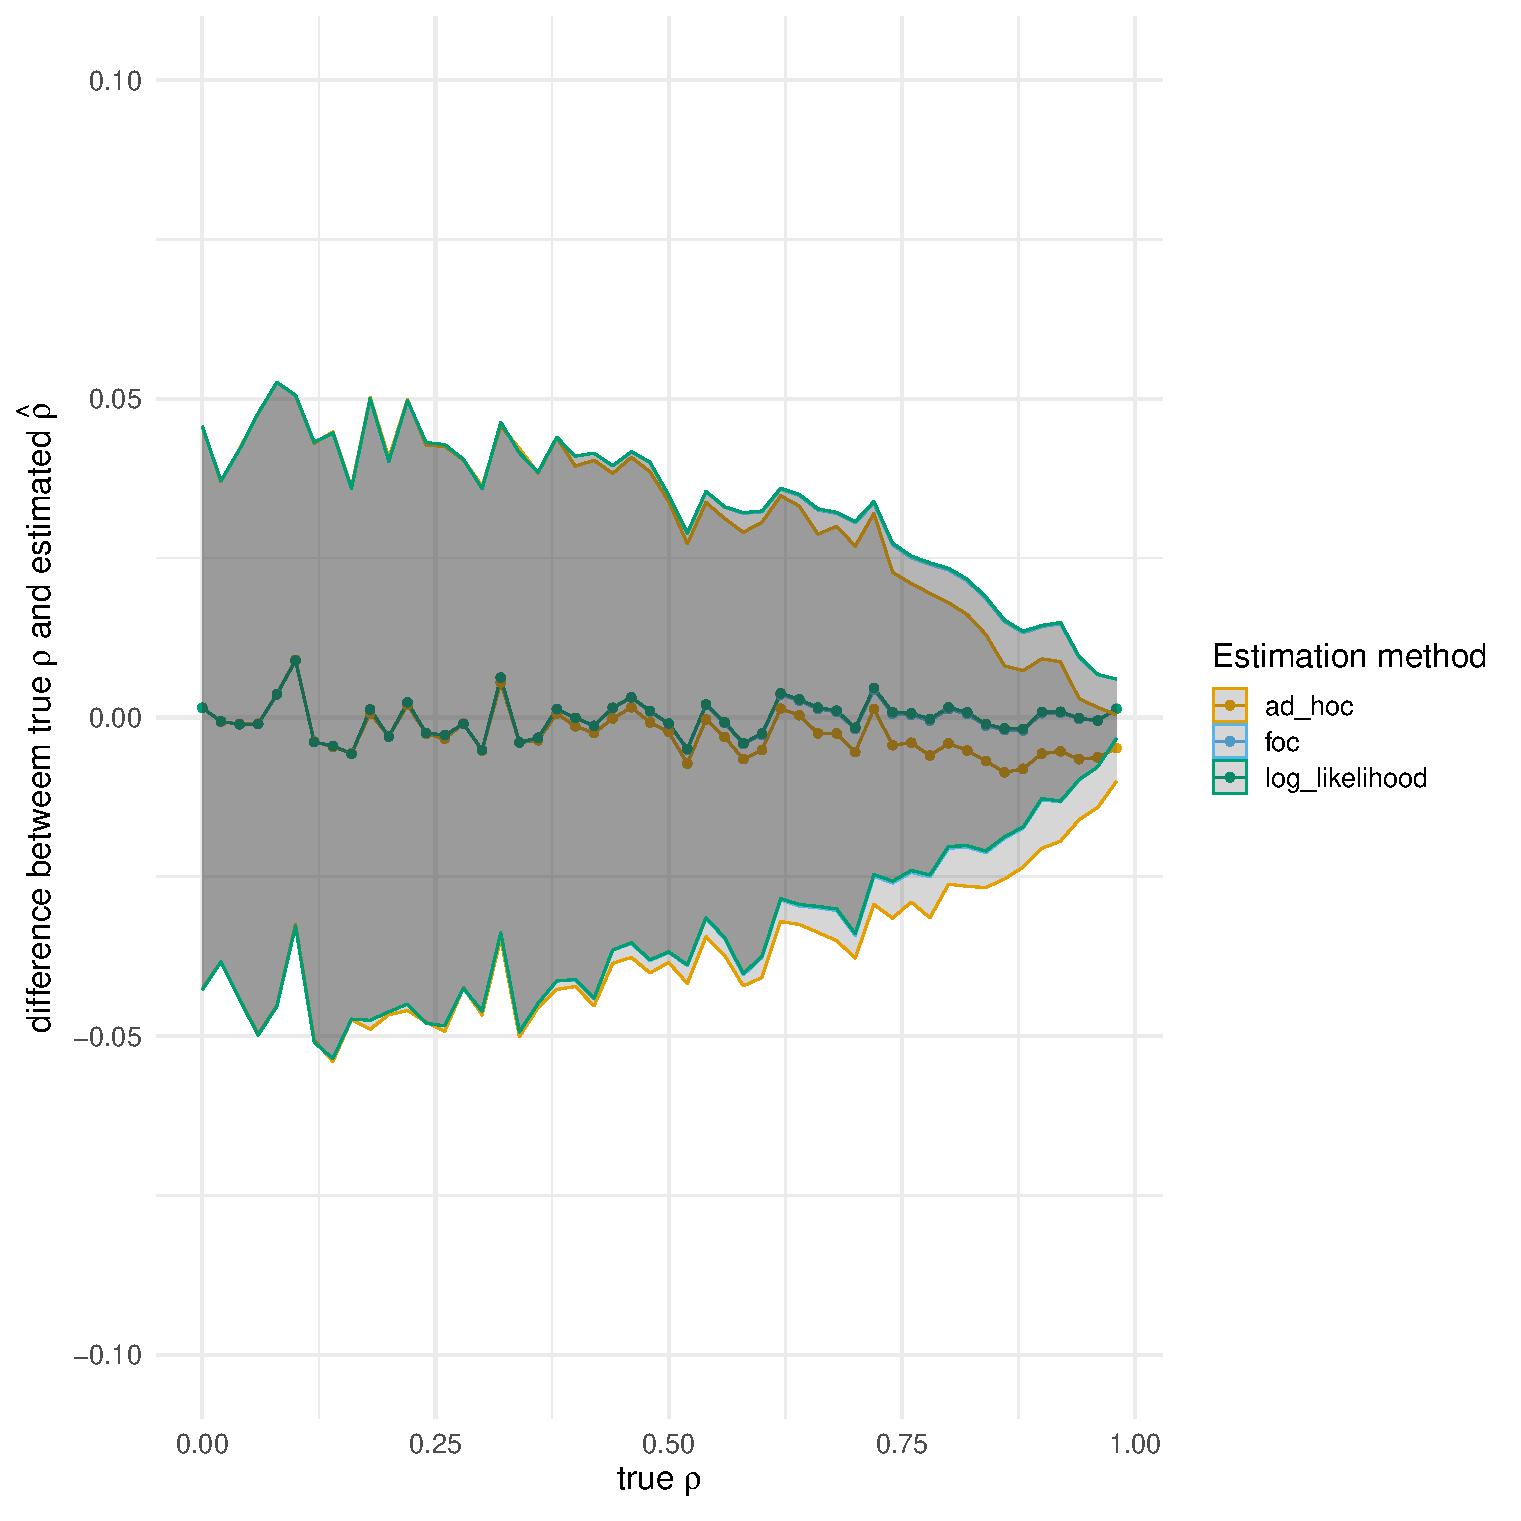
\includegraphics[width=\textwidth]{Figures/case_2_difference.pdf}
    \caption{Comparison of the \textit{Case II} MLE under the LGCM and the ad-hoc estimator.}
\end{figure}

As expected, both strategies for attaining the MLE yield the same results. The ad-hoc estimator's bias shows only when the underlying correlation \(\Sigma^*_{jk}\) exceeds \(0.75\) and it remains at such a mild level that we consider it negligible \citep[see][for a similar observation]{Olsson82}. The strength of the ad-hoc estimator lies in its simplicity and computational efficiency. The left panel of \figref{fig:case2_speed} shows the median, first and third quartile computation time and for the MLE and the ad-hoc estimator for a grid of sample sizes \(n \in [50, 10000]\) with a step size of \(s_t = 50\). Here we fix \(\Sigma^*_{jk} = .87\) and repeat each calculation \(100\) times recording the time elapsed.

\begin{figure}\label{fig:case2_speed}
    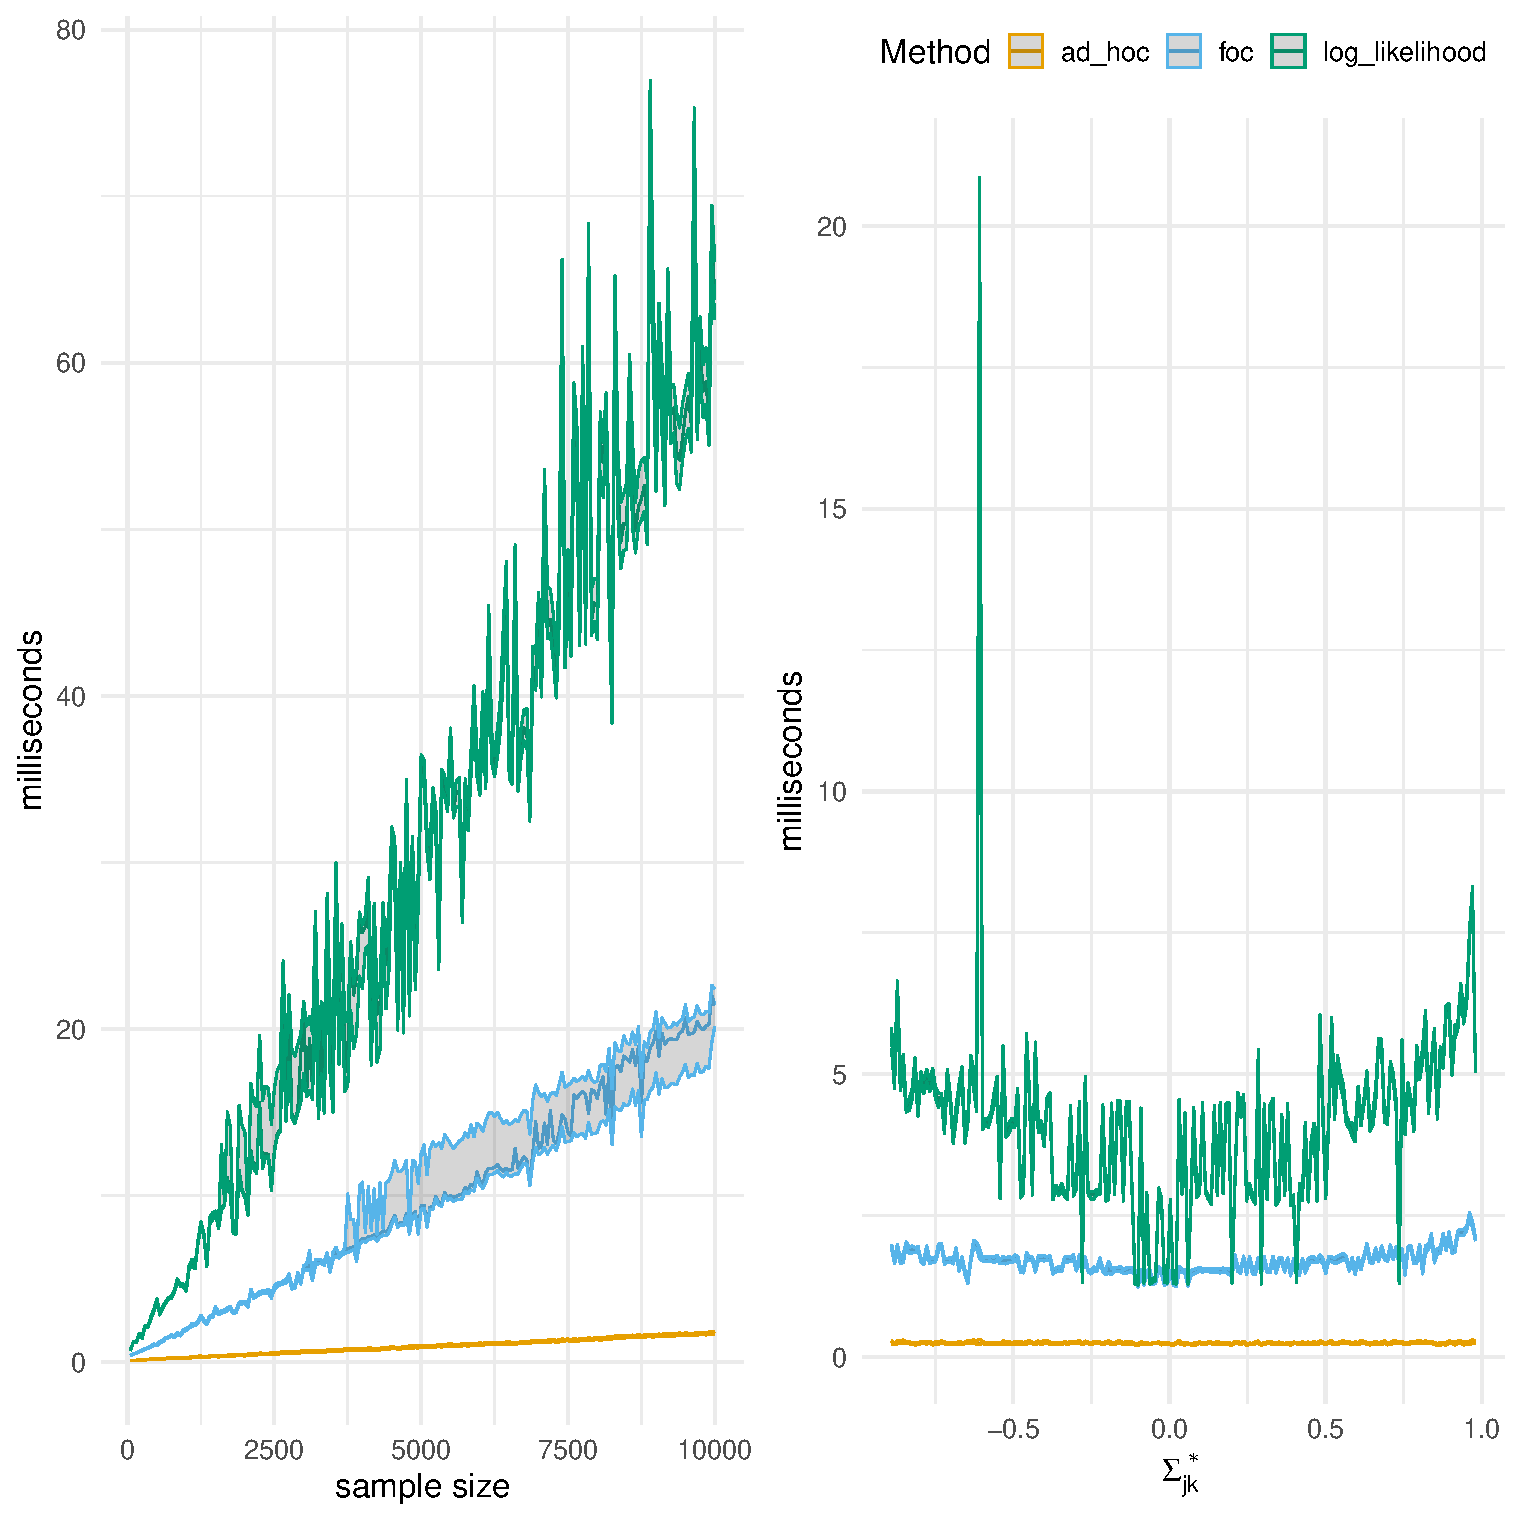
\includegraphics[width=\textwidth]{Figures/case_2_speed_comp.pdf}
    \caption{Computation time in milliseconds for the \textit{Case II} MLE and ad-hoc estimators. We report the median (solid line) and the first and third quartile (shaded area) of recorded computation time. In the left panel, we compare computation time against a grid of sample sizes \(n \in [50, 10000]\) with a step size of \(s_t = 50\). In the right panel, we compare computation time against a grid of true correlation values \(\Sigma^*_{jk} \in [-.98, .98]\).}
\end{figure}

The right panel of \figref{fig:case2_speed} demonstrates computation time across a grid of length \(200\) of values for \(\Sigma_{jk}^* \in [-.98, 98]\). The sample size is, in this case, fixed at \(n=1000\). The ad-hoc estimator is consistently and considerably faster than the MLE, regardless of the strategy used. The difference in computation time is especially pronounced for large sample sizes and correlation values approaching the endpoints of the $[-1,1]$-interval. Setting the FOC to zero and solving for \(\Sigma_{jk}\) is computationally more efficient than directly maximizing the log-likelihood function. The time difference in MLE strategies is more pronounced at the endpoints of the $[-1,1]$ interval. The ad-hoc estimator is not affected by this issue. Therefore, in the high-dimensional setting we consider in this paper, the ad-hoc estimator is preferable to the MLE due to (1) its computational efficiency, (2) its simplicity, which allows us to form concentration inequalities, and (3) its robustness to the underlying correlation value.

%\section{\textit{Case II} under the Gaussian Copula model}

%Assume that $E[X_k \mid Z_j] = \mu_{k} + \Sigma_{jk}^*\sigma_{k}Z_j$ for $j \in d_1+1, \dots, d_2$ and $k \in 1, \dots, d_1$ and that the standardized continuous and the latent continuous variable are identically distributed, i.e. $X_k \sim Z_j$.

%Denote $\Xi(t) = P((X_k - \mu_k)/\sigma_k \leq t)$ and set $\lambda(\Xi; x^j, \xi^j) = \sum_{r=1}^{l_{j}} x^r_j \int_{\xi_{r-1}^{j}}^{\xi_{r}^{j}} z d\Xi(z)$ where $\xi^j = (\xi_j^0, \xi^j_1, \dots, \xi_j^{l_j +1})^\prime$ and $\xi^r_j = \Xi^{-1}(p_{\cdot r}^j)$ then by \citet[p. 430]{Bedrick96} we obtain
%\begin{equation}\label{eq:polyserial_adhoc}
%    \Sigma_{jk}^* = \frac{\rho_{X_j X_k} \sigma_j}{\lambda(\Xi; x^j, \xi^j)}.
%\end{equation}

%We need to find sample equivalences for each component in Eq. \eqref{eq:polyserial_adhoc}. As the numerator does not change compared to the naive approach, let us focus on $\lambda(\Xi; x^j, \xi^j)$. First, let $\tilde{\Xi}(t) = 1/n\sum_{i=1}^n \mathbbm{1}_{(X_k - \mu_k)/\sigma_k \leq t}$ be the empirical distribution function of the standardized observed continuous variable $X_k$. In order to estimate the threshold parameters $\xi^j$ we need to evaluate percentiles of $\tilde{X}_k$, i.e, $\hat{\xi}^r_j = \tilde{\Xi}^{-1}(p_{\cdot r}^j)$. The $X_k$'s are unique, with probability tending to one. Hence, we can estimate the corresponding percentiles using order statistics, i.e.
%\begin{equation*}
%    \tilde{\Xi}^{-1}\Big(\frac{c}{n}\Big) = \frac{(X_{k(c+1)} - X_{k(c)})/2 - %\Bar{X}_k}{\hat{\sigma}_k} \quad \text{for } c= 0,1, \dots, n,
%\end{equation*}
%where $X_{k(c)}$ denotes the $c^{th}$ order statistic of the random variable $X_k$ \citep[see][for more details]{David03}. Furthermore, we set $\tilde{\Xi}^{-1}\Big(\frac{c}{n}\Big)$ to $-\infty$ and $+\infty$ for $c=0$ and $c=n$, respectively.

%Finally, we can construct a sample estimate of $\lambda(\Xi; x^j, \xi^j)$, namely:
%\begin{equation*}
%    \lambda(\tilde{\Xi}; x^j, \hat{\xi}^j) = \sum_{r=1}^{l_{j}} x^r_j \int_{\hat{\xi}_{r-1}^{j}}^{\hat{\xi}_{r}^{j}} z d\tilde{\Xi}(z) = \frac{1}{n\hat{\sigma}_k}\sum_{r=1}^{l_{j}} x^r_j \sum_{c=1+np_{\cdot r-1}^j}^{np_{\cdot r-1}^j}(X_{k(c)} - \Bar{X}_k),
%\end{equation*}
%where equality only holds when the $X_k$'s are all distinct. In practice, when ties are present, we still use the right-most summation expression and make sure that null sums are set to zero whenever $p_{\cdot r-1}^j = p_{\cdot r}^j$. Let us denote the resulting estimator
%\begin{equation}\label{eq:brogden_adhoc}
%     \hat{\Sigma}_{jk}^+ = \frac{\hat{\rho}^{\text{\textit{Sp}}}_{jk} \hat{\sigma}_j}{\lambda(\tilde{\Xi}; x^j, \hat{\xi}^j)}.
%\end{equation}
%In order to make the upper bound of $1$ more explicit, Eq. \eqref{eq:brogden_adhoc} can be rewritten such that $\Sigma_{jk}^* = \sigma_{X_j X_k} / \sigma_k \lambda(\Xi; x^j, \xi^j)$. Now, the denominator is simply the covariance between the ordered $X_j$ and $X_k$ observations which, by the rearrangement inequality \citep[Theorem 368 in][p.261]{Hardy52}, is at least as large as $\sigma_{X_j X_k}$.

%However, $\hat{\Sigma}_{jk}^+$ is unchanged by location and scale transformation i.e. $a + bX_j$ and $a + bX_k$ only so long as $b > 0$. What's more, $\hat{\Sigma}_{jk}^+$ need not be bounded by $-1$ from below. Therefore, we simply let $\hat{\Sigma}_{jk}^- = - \hat{\Sigma}_{j-k}^+$ where $\hat{\Sigma}_{j-k}^+$ indicates that we take $- X_k = -(X_{1k}, \dots X_{kn})^\prime$ rather than $X_k$. Finally, we can state the generalized ad-hoc estimator, i.e.
%\begin{equation}\label{eq:generalized_adhoc_appendix}
%    \hat{\Sigma}_{jk}^{\text{ad-hoc}} = \begin{cases}
%    \hat{\Sigma}_{jk}^+ & \text{if } \hat{\Sigma}_{jk}^+ \geq 0 \\
%    \hat{\Sigma}_{jk}^- & \text{if } \hat{\Sigma}_{jk}^+ < 0,
%    \end{cases}
%\end{equation}
%where at last $\abs{\hat{\Sigma}_{jk}^{\text{ad-hoc}}} \leq 1$. Furthermore, $\hat{\Sigma}_{jk}^{\text{ad-hoc}}$ remains unchanged when we transform $X_j$ to $a + bX_j$ and $\hat{\Sigma}_{jk}^{\text{ad-hoc}}$ becomes $sign(b)\hat{\Sigma}_{jk}^{\text{ad-hoc}}$ when we transform $X_k$ to $a + bX_k$ \citep[see also][]{Bedrick96}.

\section{Proof of Theorem 3.2
  %\ref{uniform_convergence}
 }\label{proof_convergence}

\begin{condition}[Gradient statistical noise]\label{Gradient statistical noise}
    The gradient of the log-likelihood function is $\tau^2$-sub-Gaussian. That is, for any $\lambda \in \mathbb{R}$ and for all $\Sigma_{jk} \in [-1+\delta, 1-\delta]$ for $j,k$ according to \textit{Case II} or \textit{Case III}.
    \begin{equation}
        \mathbb{E}\Bigg[\exp\Bigg(\lambda \Big(\frac{\partial\ell_{jk}}{\partial \Sigma_{jk}} - \mathbb{E}\frac{\partial\ell_{jk}}{\partial \Sigma_{jk}} \Big) \Bigg)\Bigg] \leq \exp\Big(\frac{\tau^2\lambda^2}{2}\Big),
    \end{equation}
    where $\ell_{jk}$ corresponds to the log-likelihood functions in Definitions 2.3 and 2.4 of the main Manuscript, respectively.\todo{Numbering still correct?}
    %\ref{definition_case2} and \ref{definition_case3}.
    \paragraph{\textit{Case II}}: Recall that
    \begin{equation*}
        \frac{\partial\ell_{jk}(\Sigma_{jk}, x_j^r,x_k)}{\partial \Sigma_{jk}} = \frac{1}{p(x_{ij}^{r} \mid x_{ik}, \Sigma_{jk})} \frac{\partial p(x_{ij}^{r} \mid x_{ik}, \Sigma_{jk})}{\partial \Sigma_{jk}}.
    \end{equation*}
    Replacing these with the derivations made in Eq. \eqref{MLE_polyserial}, we write
    \begin{multline*}
        \frac{\partial\ell_{jk}(\Sigma_{jk}, x_j^r,x_k)}{\partial \Sigma_{jk}} = \\
        \frac{(1-(\Sigma_{jk})^2)^{-\frac{3}{2}}}{\Phi({\tilde{\Gamma}}_j^{r}) - \Phi({\tilde{\Gamma}}_j^{r-1})} \Bigg[\phi({\tilde{\Gamma}}_j^{r})({\Gamma}_j^r\Sigma_{jk} - {\tilde{x}}_{k}) - \phi({\tilde{\Gamma}}_j^{r-1})({\Gamma}_j^{r-1}\Sigma_{jk} - {\tilde{x}}_{k})\Bigg].
    \end{multline*}
    It is easy to see that $p(x_{ij}^{r} \mid x_{ik}, \Sigma_{jk}) \in (0,1)$ almost surely. Assumption 3.3
    %\ref{ass3} %
    makes sure that we exclude impossible events where $p(x_{ij}^{r} \mid x_{ik}, \Sigma_{jk}) = 0$. Moreover, we require that $\Gamma_j^r > \Gamma_j^{r-1}, \forall j \in 1, \dots, d_1$ this implies that $\Phi({\tilde{\Gamma}}_j^{r}) > \Phi({\tilde{\Gamma}}_j^{r-1})$. In other words, there exists a $\kappa >0$ such that $p(x_{ij}^{r} \mid x_{ik}, \Sigma_{jk}) \leq \frac{1}{\kappa}$.

    Let us now turn to $\partial p(x_{ij}^{r} \mid x_{ik}, \Sigma_{jk})/\partial \Sigma_{jk}$. First, for all $\Sigma_{jk} \in [-1+\delta, 1-\delta]$ we clearly have $1 \leq (1-(\Sigma_{jk})^2)^{-\frac{3}{2}} \leq \varpi$ for $\varpi > 1$. What's more, the density of the standard normal is bounded, i.e., $\abs{\phi(t)} \leq (2\pi)^{-\frac{1}{2}}$ for all $t \in \mathbb{R}$. Similarly,
    \begin{equation*}
        \abs{\phi({\tilde{\Gamma}}_j^{r})({\Gamma}_j^r\Sigma_{jk} - {\tilde{x}}_{k}) - \phi({\tilde{\Gamma}}_j^{r-1})({\Gamma}_j^{r-1}\Sigma_{jk} - {\tilde{x}}_{k})} \leq  \abs{\phi({\tilde{\Gamma}}_j^{r})({\Gamma}_j^r\Sigma_{jk} - {\tilde{x}}_{k})} \leq L_1,
    \end{equation*}
    due to Assumption 3.2. %\ref{ass2}.
    Therefore,
    \begin{equation*}
        \abs{\frac{\partial\ell_{jk}(\Sigma_{jk}, x_j^r,x_k)}{\partial \Sigma_{jk}}} \leq \kappa L_1,
    \end{equation*}
    and $\Big(\frac{\partial\ell_{jk}}{\partial \Sigma_{jk}} - \mathbb{E}\frac{\partial\ell_{jk}}{\partial \Sigma_{jk}} \Big)$ is zero-mean and bounded. Then by Hoeffding's (\citeyear{Hoeffding63}) lemma  the gradient of the log-likelihood function is $\tau^2$-sub-Gaussian with $\tau = 2\kappa L_1$

    \paragraph{\textit{Case III}}: Recall that we have
    \begin{equation*}
        \frac{\partial \ell_{jk}(\Sigma_{jk}, x_j^r,x_k^s)}{\partial \Sigma_{jk}} = \frac{1}{\pi_{rs}} \frac{\partial \pi_{rs}}{\partial \Sigma_{jk}}, \quad \text{for some }j<k \in [d_1].
    \end{equation*}
    Considering
    \begin{align*}
        \pi_{rs} = & \Phi_2({\Gamma}_j^r, {\Gamma}_k^s, \Sigma_{jk}) - \Phi_2({\Gamma}_j^{r-1}, {\Gamma}_k^s, \Sigma_{jk})          \\
        -          & \Phi_2({\Gamma}_j^r, {\Gamma}_k^{s-1}, \Sigma_{jk}) + \Phi_2({\Gamma}_j^{r-1}, {\Gamma}_k^{s-1}, \Sigma_{jk}),
    \end{align*}
    we note that this again has to be in $(0,1)$ due to Assumptions 3.1 and 3.2,
    % \ref{ass1} and \ref{ass2}.
    such that $\pi_{rs} \leq \frac{1}{\xi}$. %Also, the bivariate normal is bounded from above by $\min[\Phi(b)\Phi(h),\Phi(a)\Phi(k)]$ where $a=\frac{h-\rho k}{(1-\rho^2)^{1/2}}$ and $b=\frac{k-\rho h}{(1-\rho^2)^{1/2}}$

    Now let us show that
    \begin{align*}
        \frac{\partial \pi_{rs}}{\partial \Sigma_{jk}}
        = \Big[ & \phi_2({\Gamma}_j^r, {\Gamma}_k^s, \Sigma_{jk}) - \phi_2({\Gamma}_j^{r-1}, {\Gamma}_k^s, \Sigma_{jk})              \\
        -       & \phi_2({\Gamma}_j^r, {\Gamma}_k^{s-1}, \Sigma_{jk}) + \phi_2({\Gamma}_j^{r-1}, {\Gamma}_k^{s-1}, \Sigma_{jk})\Big]
    \end{align*}
    is bounded. Indeed, the density of the standard bivariate normal random variable is of the form $\phi_2(x,y) = c e^{-q(x,y)}$. Since $q(x,y)$ is a quadratic function of $x,y$ it follows that $\abs{\phi_2(x,y)} \leq c$. Therefore, every element in $\frac{\partial \pi_{rs}}{\partial \Sigma_{jk}}$ is bounded and thus $\abs{\frac{\partial \pi_{rs}}{\partial \Sigma_{jk}}} \leq K_1$. By the same argument as for \textit{Case II} $\Big(\frac{\partial\ell_{jk}}{\partial \Sigma_{jk}} - \mathbb{E}\frac{\partial\ell_{jk}}{\partial \Sigma_{jk}} \Big)$ is zero-mean and bounded and by Hoeffding's lemma the gradient of the log-likelihood function is $\tau^2$-sub-Gaussian with $\tau = 2\xi K_1$. Based on these arguments, we can conclude that the condition for gradient statistical noise is satisfied.
\end{condition}

\begin{condition}[Hessian statistical noise]\label{Hessian statistical noise}
    The Hessian of the log-likelihood function is $\tau^2$-sub-exponential, i.e. for all $\Sigma_{jk} \in [-1+\delta, 1-\delta]$ and for $j,k$ according to \textit{Case II} or \textit{Case III} we have
    \begin{equation}
        \norm{\frac{\partial^2\ell_{jk}}{\partial \Sigma_{jk}^{2}}}_{\psi_{1}} \leq \tau^2,
    \end{equation}
    where $\Norm{\cdot}_{\psi_{1}}$ denotes the \textit{Orlicz} $\psi_{1}$-norm, defined as
    \begin{equation*}
        \Norm{X}_{\psi_{1}} \coloneqq \sup_{p\geq 1} \frac{1}{p}\mathbb{E}\Big(\abs{X - \mathbb{E}(X)}^p\Big)^{\frac{1}{p}}.
    \end{equation*}
    Note that $\ell_{jk}$ corresponds to the respective log-likelihood functions in Definitions 2.3 and 2.4.\todo{Still correct?}% \ref{definition_case2} and \ref{definition_case3}.

    \paragraph{\textit{Case II}}: We have
    \begin{equation}\label{hessian_case2}
        \begin{split}
            \frac{\partial^2\ell_{jk}}{\partial \Sigma_{jk}^{2}} &= \frac{\partial^2 p(x_j^{r} \mid x_{k}, \Sigma_{jk})/\partial \Sigma_{jk}^{2}}{p(x_j^{r} \mid x_{k}, \Sigma_{jk})} - \Bigg(\frac{\partial p(x_j^{r} \mid x_{k}, \Sigma_{jk}) / \partial \Sigma_{jk}}{p(x_j^{r} \mid x_{k}, \Sigma_{jk})}\Bigg)^2. \\
            \text{Clearly, } \abs{\frac{\partial^2\ell_{jk}}{\partial \Sigma_{jk}^{2}}} &\leq \frac{\abs{\partial^2 p(x_j^{r} \mid x_{k}, \Sigma_{jk})/\partial \Sigma_{jk}^{2}}}{\abs{p(x_j^{r} \mid x_{k}, \Sigma_{jk})}} + \Bigg( \frac{\abs{\partial p(x_j^{r} \mid x_{k}, \Sigma_{jk}) / \partial \Sigma_{jk}}}{\abs{p(x_j^{r} \mid x_{k}, \Sigma_{jk})}} \Bigg)^2 \\
            &\leq \kappa L_2 + \kappa^2 L_1^2,
        \end{split}
    \end{equation}
    where it remains to show that $\abs{\partial^2 p(x_{ij}^{r} \mid x_{ik}, \Sigma_{jk})/\partial \Sigma_{jk}^{2}} \leq L_2$. Indeed, we can rewrite our objective as follows:
    \begin{multline}\label{second_derivative_case2}
        \frac{\partial}{\partial \Sigma_{jk}} \Bigg(\frac{\partial\ell_{jk}(\Sigma_{jk}, x_j^r,x_k)}{\partial \Sigma_{jk}}\Bigg) \\
        \begin{aligned}
             & = \frac{\partial}{\partial \Sigma_{jk}}\Bigg( (1-(\Sigma_{jk})^2)^{-\frac{3}{2}} \Bigg[\phi({\tilde{\Gamma}}_j^{r})({\Gamma}_j^r\Sigma_{jk} - {\tilde{x}}_{k}) - \phi({\tilde{\Gamma}}_j^{r-1})({\Gamma}_j^{r-1}\Sigma_{jk} - {\tilde{x}}_{k})\Bigg] \Bigg)      \\
            %
             & = \frac{3\Sigma_{jk}}{1-\Sigma_{jk}^2} (1-(\Sigma_{jk})^2)^{-\frac{3}{2}} \phi({\tilde{\Gamma}}_j^{r})({\Gamma}_j^r\Sigma_{jk} - {\tilde{x}}_{k}) + \frac{\phi^\prime({\tilde{\Gamma}}_j^{r})({\Gamma}_j^r\Sigma_{jk} - {\tilde{x}}_{k})^2}{(1-\Sigma_{jk}^2)^3} \\
            %
             & + \frac{\phi({\tilde{\Gamma}}_j^{r}){\Gamma}_j^{r}}{(1-\Sigma_{jk}^2)^{-\frac{3}{2}}} - \frac{3\Sigma_{jk}}{1-\Sigma_{jk}^2} (1-(\Sigma_{jk})^2)^{-\frac{3}{2}} \phi({\tilde{\Gamma}}_j^{r-1})({\Gamma}_j^{r-1}\Sigma_{jk} - {\tilde{x}}_{k})                    \\
            %
             & -  \frac{\phi^\prime({\tilde{\Gamma}}_j^{r-1})({\Gamma}_j^{r-1}\Sigma_{jk} - {\tilde{x}}_{k})^2}{(1-\Sigma_{jk}^2)^3} - \frac{\phi({\tilde{\Gamma}}_j^{r-1}){\Gamma}_j^{r-1}}{(1-\Sigma_{jk}^2)^{-\frac{3}{2}}}.
        \end{aligned}
    \end{multline}
    \begin{equation*}
        \begin{split}
            \text{Thus: } \abs{\frac{\partial}{\partial \Sigma_{jk}} \Bigg(\frac{\partial\ell_{jk}(\Sigma_{jk}, x_j^r,x_k)}{\partial \Sigma_{jk}}\Bigg)} \leq &\abs{\frac{3\Sigma_{jk}}{1-\Sigma_{jk}^2} (1-(\Sigma_{jk})^2)^{-\frac{3}{2}} \phi({\tilde{\Gamma}}_j^{r})({\Gamma}_j^r\Sigma_{jk} - {\tilde{x}}_{k})} \\
            + &\abs{\frac{\phi^\prime({\tilde{\Gamma}}_j^{r})({\Gamma}_j^r\Sigma_{jk} - {\tilde{x}}_{k})^2}{(1-\Sigma_{jk}^2)^3} + \frac{\phi({\tilde{\Gamma}}_j^{r}){\Gamma}_j^{r}}{(1-\Sigma_{jk}^2)^{-\frac{3}{2}}}} \leq L_2,
        \end{split}
    \end{equation*}
    due to Assumptions 3.1 and 3.2\todo{Check numeration.} % \ref{ass1} and \ref{ass2} %
    and because both $\phi(t)$ and $\phi^{\prime}(t)$ are bounded for all $t\in\mathbb{R}$. Therefore, the inequality in Eq. \eqref{hessian_case2} follows and $\frac{\partial^2\ell_{jk}}{\partial \Sigma_{jk}^{2}} - \mathbb{E}\bigg(\frac{\partial^2\ell_{jk}}{\partial \Sigma_{jk}^{2}}\bigg)$ is bounded by $2(\kappa L_2 + \kappa^2 L_1^2)$. Hence, for all $p\geq1$
    \begin{equation}
        \frac{1}{p}\mathbb{E}\Bigg[\abs{\partial^2\ell_{jk}/\partial \Sigma_{jk}^{2} - \mathbb{E}\big(\partial^2\ell_{jk}/\partial \Sigma_{jk}^{2}\big)}^p\Bigg]^{\frac{1}{p}} \leq \frac{2}{p}\big(\kappa L_2 + \kappa^2 L_1^2\big).
    \end{equation}
    Finally, for $\tau = 2\kappa L_1$ we can choose $L_1$ and $\kappa$ such that \[2(\kappa L_2 + \kappa^2 L_1^2) \leq \tau^2 = 4\kappa^2 L_1^2.\] Thus, the \textit{Hessian statistical noise}-condition for \textit{Case II} is satisfied.

    \paragraph{\textit{Case III}:} Let us start with the Hessian of \(\ell_{jk}\) in the polychoric case:
    \begin{equation}\label{hessian_case3}
        \begin{split}
            \frac{\partial^2 \ell_{jk}(\Sigma_{jk}, x_j^r,x_k^s)}{\partial \Sigma_{jk}^{2}} &= \frac{\partial^2 \pi_{rs}/\partial \Sigma_{jk}^{2}}{\pi_{rs}} - \Bigg(\frac{\partial \pi_{rs}/\partial \Sigma_{jk}}{\pi_{rs}}\Bigg)^2 \\
            \text{Thus: } \abs{\frac{\partial^2 \ell_{jk}(\Sigma_{jk}, x_j^r,x_k^s)}{\partial \Sigma_{jk}^{2}}} &\leq \frac{\abs{\partial^2 \pi_{rs}/\partial \Sigma_{jk}^{2}}}{\abs{\pi_{rs}}} + \Bigg(\frac{\abs{\partial \pi_{rs}/\partial \Sigma_{jk}}}{\abs{\pi_{rs}}} \Bigg)^2 \\
            &\leq \xi K_2 + \xi^2K_1^2.
        \end{split}
    \end{equation}
    Again it remains to show that $\partial^2 \pi_{rs}/\partial \Sigma_{jk}^{2} \leq K_2$. Consider
    \begin{equation*}
        \begin{split}
            \lefteqn{\abs{\frac{\partial}{\partial \Sigma_{jk}}\bigg(\frac{\partial \pi_{rs}}{\partial \Sigma_{jk}}\bigg)}} \\
            &= \Big\lvert \frac{\partial}{\partial \Sigma_{jk}}\phi_2({\Gamma}_j^r, {\Gamma}_k^s, \Sigma_{jk}) - \phi_2({\Gamma}_j^{r-1}, {\Gamma}_k^s, \Sigma_{jk}) \\
            &- \phi_2({\Gamma}_j^r, {\Gamma}_k^{s-1}, \Sigma_{jk}) + \phi_2({\Gamma}_j^{r-1}, {\Gamma}_k^{s-1}, \Sigma_{jk})\Big\rvert \\
            &\leq \abs{\frac{\partial}{\partial \Sigma_{jk}}\phi_2({\Gamma}_j^r, {\Gamma}_k^s, \Sigma_{jk})} + \abs{\frac{\partial}{\partial \Sigma_{jk}}\phi_2({\Gamma}_j^{r-1}, {\Gamma}_k^s, \Sigma_{jk})} \\
            &+ \abs{\frac{\partial}{\partial \Sigma_{jk}}\phi_2({\Gamma}_j^r, {\Gamma}_k^{s-1}, \Sigma_{jk})} + \abs{\frac{\partial}{\partial \Sigma_{jk}}\phi_2({\Gamma}_j^{r-1}, {\Gamma}_k^{s-1}, \Sigma_{jk})} \\
            &\leq K_2,
        \end{split}
    \end{equation*}
    where each of the derivatives of the bivariate density is bounded, since we assume that the correlation is bounded away from one and minus one, i.e., \(\Sigma_{jk} \in [-1 + \delta, 1 - \delta]\).

    Similar to \textit{Case II}, for $\tau = 2\xi K_1$ we can choose $K_1$ and $\xi$ such that \[2(\xi k_2 + \xi^2 k_1^2) \leq \tau^2 = 4\xi^2 K_1^2.\]
    Consequently, the \textit{Hessian statistical noise}-condition for \textit{Case III} is satisfied, which concludes the proof of the \textit{Hessian statistical noise}-condition.
\end{condition}

Concerning the third condition, we introduce some additional notation. Denote the sample risk by $\hat{R}_{jk}^{(n)}(\Sigma_{jk})$ for \(j,k\) according to \textit{Case II} and \textit{Case III}, i.e.,
\begin{equation*}
    \text{\textit{Case II}:} \quad \hat{R}_{jk}^{(n)}(\Sigma_{jk}) = \frac{1}{n} \sum_{i=1}^n \big[\log(p(x_{ik})) + \log(p(x_{ij}^{r} \mid x_{ik}, \Sigma_{jk}))\big],
\end{equation*}
and
\begin{equation*}
    \text{\textit{Case III}:} \quad \hat{R}_{jk}^{(n)}(\Sigma_{jk}) = \frac{1}{n} \sum_{r=1}^{l_{X_{j}}}\sum_{s=1}^{l_{X_{k}}} n_{rs} \log(\pi_{rs}).
\end{equation*}
Lastly, we define $R_{jk}(\Sigma_{jk}) = \mathbb{E}_{\Sigma_{jk}^*}\hat{R}_{jk}^{(n)}(\Sigma_{jk})$ to be the population risk for each of the respective cases.
\begin{condition}[Hessian regularity]
    The Hessian regularity condition consists of three parts:
    \begin{enumerate}
        \item The second derivative of the population risk $R_{jk}(\Sigma_{jk})$ is bounded at one point. That is, there exists one $\Abs{\Bar{\Sigma}_{jk}} \leq 1- \delta$ and $H > 0$ such that $\Abs{R_{jk}^{\prime\prime}(\Bar{\Sigma}_{jk})} \leq H$.
        \item The second derivative of the log-likelihood with respect to $\Sigma_{jk}$ is Lipschitz continuous with integrable Lipschitz constant, i.e. there exists a $M^* > 0$ such that $\mathbb{E}[M] \leq M^*$, where
              \begin{equation*}
                  M = \sup_{\substack{\Abs{\Sigma_{jk}^{(1)}}, \  \Abs{\Sigma_{jk}^{(2)}} \leq 1- \delta, \\ \Sigma_{jk}^{(1)} \neq \Sigma_{jk}^{(2)}}} \frac{\abs{\ell_{jk}^{\prime\prime}(\Sigma_{jk}^{(1)}) - \ell_{jk}^{\prime\prime}(\Sigma_{jk}^{(2)})}}{\abs{\Sigma_{jk}^{(1)} - \Sigma_{jk}^{(2)}}}.
              \end{equation*}
        \item The constants $H$ and $M^*$ are such that $H \leq \tau^2$ and $M^*\leq \tau^3$.
    \end{enumerate}
    We need some intermediate results that make dealing with $R_{jk}(\Sigma_{jk})$ easier. First, note that $\mathbb{E}_{\Sigma_{jk}^*}\hat{R}_{jk}^{(n)}(\Sigma_{jk}) = \mathbb{E}_{\Sigma_{jk}^*}\ell_{jk}(\Sigma_{jk})$. Second, for all $\Sigma_{jk} \in [-1+\delta, 1-\delta]$ and $m \in \{1,2\}$
    \begin{equation*}
        R_{jk}^m(\Sigma_{jk}) = \frac{\partial^m}{\partial\Sigma_{jk}^m}\mathbb{E}_{\Sigma_{jk}^*}\ell_{jk}(\Sigma_{jk}) = \mathbb{E}_{\Sigma_{jk}^*}\frac{\partial^m}{\partial\Sigma_{jk}^m}\ell_{jk}(\Sigma_{jk}),
    \end{equation*}
    by Lemma \ref{expectation_commutes_case2} and Corollary \ref{expectation_commutes_case3}.

    \begin{enumerate}
        \item Recall the first part of the Hessian regularity condition, whereby Eq. \eqref{hessian_case2} and Eq. \eqref{hessian_case3} for all $\Sigma_{jk} \in [-1+\delta, 1-\delta]$ we have
              \[\text{\textit{Case II}:} \quad \Abs{\frac{\partial^2}{\partial\Sigma_{jk}^2}\ell_{jk}(\Sigma_{jk})} \leq \kappa L_2 + \kappa^2L_1^2\]
              and
              \[\text{\textit{Case III}:} \quad \Abs{\frac{\partial^2}{\partial\Sigma_{jk}^2}\ell_{jk}(\Sigma_{jk})} \leq \xi K_2 + \xi^2K_1^2\] for cases II and III, respectively. Consequently, the claim in the first part of the Hessian regularity condition holds for \textit{Case II} and \textit{Case III} for any $\Abs{\Bar{\Sigma}_{jk}} \leq 1-\delta$ with $H_{1} = \kappa L_2 + \kappa^2L_1^2$ and $H_{2} = \xi K_2 + \xi^2K_1^2$. Moreover, we also have $H_1 \leq \tau^2 = 4\kappa^2L_1^2$ and $H_2 \leq \tau^2 = 4\xi^2K_1^2$.

        \item The second part of the Hessian regularity condition requires that the second derivative of the log-likelihood with respect to $\Sigma_{jk}$ is Lipschitz continuous with integrable Lipschitz constant. By the mean-value-theorem, all we need to show is that we can find a bound on the third derivative of the log-likelihood function.

              \paragraph{\textit{Case II}:} Note that we have
              \begin{align*}
                  \MoveEqLeft \frac{\partial^3}{\partial\Sigma_{jk}^3}\ell_{jk}(\Sigma_{jk})                                                                                                                                                                                                                           \\
                   & = \frac{\partial}{\partial\Sigma_{jk}}\Bigg[\frac{\partial^2\ell_{jk}}{\partial \Sigma_{jk}^{2}}\Bigg]                                                                                                                                                                                            \\
                   & = \frac{\partial}{\partial\Sigma_{jk}}\Bigg[\frac{\partial^2 p(x_j^{r} \mid x_{k}, \Sigma_{jk})/\partial \Sigma_{jk}^{2}}{p(x_j^{r} \mid x_{k}, \Sigma_{jk})} - \Bigg(\frac{\partial p(x_j^{r} \mid x_{k}, \Sigma_{jk}) / \partial \Sigma_{jk}}{p(x_j^{r} \mid x_{k}, \Sigma_{jk})}\Bigg)^2\Bigg] \\
                   & = \frac{\partial^3 p(x_j^{r} \mid x_{k}, \Sigma_{jk}) / \partial \Sigma_{jk}^3}{p(x_j^{r} \mid x_{k}, \Sigma_{jk})}                                                                                                                                                                               \\
                   & - 3\frac{\big(\partial p(x_j^{r} \mid x_{k}, \Sigma_{jk}) / \partial \Sigma_{jk}\big)\big( \partial^2 p(x_j^{r} \mid x_{k}, \Sigma_{jk}) / \partial \Sigma_{jk}^2\big)}{(p(x_j^{r} \mid x_{k}, \Sigma_{jk}))^2}                                                                                   \\
                   & +  2\Bigg(\frac{\partial p(x_j^{r} \mid x_{k}, \Sigma_{jk}) / \partial \Sigma_{jk}}{p(x_j^{r} \mid x_{k}, \Sigma_{jk})}\Bigg)^3.
              \end{align*}
              Hence \[\abs{\frac{\partial^3}{\partial\Sigma_{jk}^3}\ell_{jk}(\Sigma_{jk})}
                  \leq \kappa L_3 + 3\kappa^2L_2L_1 + 2 \kappa^3L_1^3.\]
              It remains to show therefore, that \[\abs{\partial^3 p(x_j^{r} \mid x_{k}, \Sigma_{jk}) / \partial \Sigma_{jk}^3} \leq L_3.\]
              When taking the derivative of Eq. \eqref{second_derivative_case2}, it is obvious that the resulting statement is bounded due to Assumptions 3.1 and 3.2
              %\ref{ass1} and \ref{ass2} %
              and the fact that $\phi(t), \phi^\prime(t), \phi^{\prime\prime}(t)$ are all bounded for all $t \in \mathbb{R}$.

              Therefore, by applying the mean-value-theorem we get \[M_1 \leq \kappa L_3 + 3\kappa^2L_2L_1 + 2 \kappa^3L_1^3,\]
              and the natural choice for \[M_1^* = \kappa L_3 + 3\kappa^2L_2L_1 + 2 \kappa^3L_1^3,\] where it follows that \[M_1^* \leq \tau^3 = 8\kappa^3L_1^3.\]

              \paragraph{\textit{Case III}:} We proceed similarly and first consider
              \begin{align}
                  \begin{split}
                      \MoveEqLeft \frac{\partial^3}{\partial\Sigma_{jk}^3}\ell_{jk}(\Sigma_{jk}) \\
                      & = \frac{\partial}{\partial\Sigma_{jk}}\Bigg[\frac{\partial^2 \ell_{jk}(\Sigma_{jk}, x_j^r,x_k^s)}{\partial \Sigma_{jk}^{2}}\Bigg] \\
                      &= \frac{\partial}{\partial\Sigma_{jk}}\Bigg[\frac{\partial^2 \pi_{rs}/\partial \Sigma_{jk}^{2}}{\pi_{rs}} - \Bigg(\frac{\partial \pi_{rs}/\partial \Sigma_{jk}}{\pi_{rs}}\Bigg)^2\Bigg] \\
                      &= \frac{\partial^3 \pi_{rs} / \partial \Sigma_{jk}^3}{\pi_{rs}} - 3\frac{\big(\partial \pi_{rs} / \partial \Sigma_{jk}\big)\big( \partial^2 \pi_{rs} / \partial \Sigma_{jk}^2\big)}{(\pi_{rs})^2} \\
                      &+ 2\Bigg(\frac{\partial \pi_{rs} / \partial \Sigma_{jk}}{\pi_{rs}}\Bigg)^3.
                  \end{split}
              \end{align}
              Hence \[\abs{\frac{\partial^3}{\partial\Sigma_{jk}^3}\ell_{jk}(\Sigma_{jk})} \leq \xi K_3 + 3\xi^2K_2K_1 + 2 \xi^3K_1^3.\]
              Taking a closer look at $\abs{\partial^3 \pi_{rs} / \partial \Sigma_{jk}^3}$, boundedness again follows from the fact that the quadratic function in the exponential of the bivariate normal density does not vanish. Thus, we have \[M_2 \leq \xi K_3 + 3\xi^2K_2K_1 + 2 \xi^3K_1^3,\] and the natural choice for \[M_2^* = \xi K_3 + 3\xi^2K_2K_1 + 2 \xi^3K_1^3,\] where we have \[M_2^* \leq \tau^3 = 8\xi^3K_1^3.\] These steps validate the \textit{Hessian regularity} condition.
    \end{enumerate}

    \begin{condition}[Population risk is strongly Morse]
        There exist $\epsilon > 0$ and $\eta > 0$ such that $R_{jk}(\Sigma_{jk})$ is $(\epsilon,\eta)$\textit{-strongly Morse}, i.e.
        \begin{enumerate}
            \item For all $\Sigma_{jk}$ such that $\Abs{\Sigma_{jk}} = 1-\delta$ we have that $\Abs{R_{jk}^\prime(\Sigma_{jk})} > \epsilon$.
            \item For all $\Sigma_{jk}$ such that $\Abs{\Sigma_{jk}} \leq 1-\delta$: \[ \Abs{R_{jk}^\prime(\Sigma_{jk})} \leq \epsilon \implies \Abs{R_{jk}^{\prime\prime}(\Sigma_{jk})} \geq \eta.\]
        \end{enumerate}
        Put differently, $R_{jk}(\Sigma_{jk})$ is $(\epsilon,\eta)$\textit{-strongly Morse} if the boundaries $\{-1+ \delta, 1-\delta\}$ are not critical points of $R_{jk}(\Sigma_{jk})$ and if $R_{jk}(\Sigma_{jk})$ only has finitely many critical points that are all non-degenerate.

        Let us verify that $R^{\prime\prime}(\Sigma_{jk}) \neq 0$ for cases II and III. Indeed by Lemma \ref{expectation_commutes_case2} and Corollary \ref{expectation_commutes_case3} we can rewrite $R_{jk}^{\prime\prime}(\Sigma_{jk})$ and obtain
        \begin{align*}
            \MoveEqLeft R^{\prime\prime}(\Sigma_{jk})                                                                                                                                                                                                                                                                                                     \\
             & = \mathbb{E}_{\Sigma_{jk}}\Bigg[\frac{\partial^2 \ell_{jk}(\Sigma_{jk})}{\partial\Sigma_{jk}^2}\Bigg]                                                                                                                                                                                                                                      \\
             & = \mathbb{E}_{\Sigma_{jk}^*} \begin{dcases*}
                                                \frac{\partial^2 p(x_j^{r} \mid x_{k}, \Sigma_{jk})/\partial \Sigma_{jk}^{2}}{p(x_j^{r} \mid x_{k}, \Sigma_{jk})} - \Bigg(\frac{\partial p(x_j^{r} \mid x_{k}, \Sigma_{jk}) / \partial \Sigma_{jk}}{p(x_j^{r} \mid x_{k}, \Sigma_{jk})}\Bigg)^2 & \text{\textit{Case II}},  \\
                                                \frac{\partial^2 \pi(\Sigma_{jk})_{rs}/\partial \Sigma_{jk}^{2}}{\pi(\Sigma_{jk})_{rs}} - \Bigg(\frac{\partial \pi(\Sigma_{jk})_{rs}/\partial \Sigma_{jk}}{\pi(\Sigma_{jk})_{rs}}\Bigg)^2                                                       & \text{\textit{Case III}},
                                            \end{dcases*}
        \end{align*}
        where in $\pi(\Sigma_{jk})_{rs}$ we made the dependence on $\Sigma_{jk}$ explicit.
        \paragraph{\textit{Case II}:} Recall that we have
        \begin{align*}
            \MoveEqLeft\mathbb{E}_{\Sigma_{jk}^*}\Bigg[\frac{\partial^2 p(x_j^{r} \mid x_{k}, \Sigma_{jk}^*)/\partial \Sigma_{jk}^{2}}{p(x_j^{r} \mid x_{k}, \Sigma_{jk}^*)}\Bigg]                                                  \\
             & = \int_{-\infty}^{\infty} \sum_{r=1}^{l_j+1} \frac{\partial^2 p(x_j^{r} \mid x_{k}, \Sigma_{jk}^*)/\partial \Sigma_{jk}^{2}}{p(x_j^{r} \mid x_{k}, \Sigma_{jk}^*)} p(x_j^{r}, x_{k}; \Sigma_{jk}^*) dx_k             \\
             & = \int_{-\infty}^{\infty} \sum_{r=1}^{l_j+1} \frac{\partial^2 p(x_j^{r} \mid x_{k}, \Sigma_{jk}^*)/\partial \Sigma_{jk}^{2}}{p(x_j^{r} \mid x_{k}, \Sigma_{jk}^*)} p(x_j^{r} \mid x_{k}, \Sigma_{jk}^*)p(x_{k}) dx_k \\
             & = \sum_{r=1}^{l_j+1} \partial^2 p(x_j^{r} \mid x_{k}, \Sigma_{jk}^*)/\partial \Sigma_{jk}^{2},
        \end{align*}
        with
        \begin{align*}
            \MoveEqLeft \sum_{r=1}^{l_j+1} \partial^2 p(x_j^{r} \mid x_{k}, \Sigma_{jk}^*)/\partial \Sigma_{jk}^{2}                                                                                                                 \\
             & =\sum_{r=1}^{l_j+1} \Bigg[ \frac{3\Sigma_{jk}}{1-\Sigma_{jk}^2} (1-(\Sigma_{jk})^2)^{-\frac{3}{2}} \phi({\tilde{\Gamma}}_j^{r})({\Gamma}_j^r\Sigma_{jk} - {\tilde{x}}_{k})                                           \\
             & + \frac{\phi^\prime({\tilde{\Gamma}}_j^{r})({\Gamma}_j^r\Sigma_{jk} - {\tilde{x}}_{k})^2}{(1-\Sigma_{jk}^2)^3} + \frac{\phi({\tilde{\Gamma}}_j^{r}){\Gamma}_j^{r}}{(1-\Sigma_{jk}^2)^{-\frac{3}{2}}}                 \\
            %
             & - \frac{3\Sigma_{jk}}{1-\Sigma_{jk}^2} (1-(\Sigma_{jk})^2)^{-\frac{3}{2}} \phi({\tilde{\Gamma}}_j^{r-1})({\Gamma}_j^{r-1}\Sigma_{jk} - {\tilde{x}}_{k})                                                              \\
             & - \frac{\phi^\prime({\tilde{\Gamma}}_j^{r-1})({\Gamma}_j^{r-1}\Sigma_{jk} - {\tilde{x}}_{k})^2}{(1-\Sigma_{jk}^2)^3} - \frac{\phi({\tilde{\Gamma}}_j^{r-1}){\Gamma}_j^{r-1}}{(1-\Sigma_{jk}^2)^{-\frac{3}{2}}}\Bigg] \\
            %
             & = 0,
        \end{align*}
        since all terms except the ones involving $\phi({\tilde{\Gamma}}_j^{0})$ and $\phi({\tilde{\Gamma}}^j_{l_j+1})$ cancel and furthermore $ \lim\limits_{t \to \pm \infty} \phi(t) = \lim\limits_{t \to \pm \infty} \phi^\prime(t) = 0$ .

        \paragraph{\textit{Case III}:} Similarly, consider
        \begin{align*}
            \MoveEqLeft \mathbb{E}_{\Sigma_{jk}^*}\Bigg[\frac{\partial^2 \pi(x_j^{r},x^k_{s}; \Sigma_{jk}^*)/\partial \Sigma_{jk}^{2}}{\pi(x_j^{r},x^k_{s}; \Sigma_{jk}^*)}\Bigg]          \\
             & = \sum_r \sum_s \Bigg[\frac{\partial^2 \pi(x_j^{r},x^k_{s}; \Sigma_{jk}^*)/\partial \Sigma_{jk}^{2}}{\pi(x_j^{r},x^k_{s}; \Sigma_{jk}^*)} P(X_j = x^r_j, X_k = x^s_k)\Bigg] \\
             & = \sum_r\sum_s \Big[\partial^2 \pi(x_j^{r},x^k_{s}; \Sigma_{jk}^*)/\partial \Sigma_{jk}^{2}\Big]                                                                            \\
             & = \sum_r\sum_s \Big[q(\Gamma_j^r, \Gamma_k^s, \Sigma_{jk}^*)\phi_2(\Gamma_j^r, \Gamma_k^s, \Sigma_{jk}^*)                                                                   \\
             & - q(\Gamma_j^{r-1}, \Gamma_k^s, \Sigma_{jk}^*)\phi_2(\Gamma_j^{r-1}, \Gamma_k^s, \Sigma_{jk}^*)                                                                             \\
             & - q(\Gamma_j^r, \Gamma_k^{s-1}, \Sigma_{jk}^*)\phi_2(\Gamma_j^r, \Gamma_k^{s-1}, \Sigma_{jk}^*)                                                                             \\
             & + q(\Gamma_j^{r-1}, \Gamma_k^{s-1}, \Sigma_{jk}^*)\phi_2(\Gamma_j^{r-1}, \Gamma_k^{s-1}, \Sigma_{jk}^*)\Big]                                                                \\
             & = q(\Gamma_j^{l_j +1}, \Gamma_k^{l_k +1}, \Sigma_{jk}^*)\phi_2(\Gamma_j^{l_j +1}, \Gamma_k^{l_k +1}, \Sigma_{jk}^*)                                                         \\
             & - q(\Gamma_j^{l_j +1}, \Gamma_k^0, \Sigma_{jk}^*)\phi_2(\Gamma_j^{l_j +1}, \Gamma_k^0, \Sigma_{jk}^*)                                                                       \\
             & - q(\Gamma_j^0, \Gamma_k^{l_k +1}, \Sigma_{jk}^*)\phi_2(\Gamma_j^0, \Gamma_k^{l_k +1}, \Sigma_{jk}^*)                                                                       \\
             & + q(\Gamma_j^0, \Gamma_k^0, \Sigma_{jk}^*)\phi_2(\Gamma_j^0, \Gamma_k^0, \Sigma_{jk}^*)                                                                                     \\
             & = 0,
        \end{align*}
        with $q(s,t,\Sigma_{jk}^*))$ denoting the corresponding quadratic function from the derivative of the bivariate normal density. As above, $\Gamma_k^{l_k+1} = \infty$ and $\Gamma_k^0 = -\infty$ for all $k \in 1, \dots d_1$. This, together with the fact that all other terms cancel when summing over $r,s$, $\phi(\cdot)$ is zero in all points containing $\Gamma_k^{l_k+1}, \Gamma_k^0$ and so the last equality follows.

        From this it follows, that $R_{jk}^{\prime\prime}(\Sigma_{jk}^*)$ can only be zero if $\partial p(x_j^{r} \mid x_{k}, \Sigma_{jk}^*) / \partial \Sigma_{jk}$ for \textit{Case II} and $\partial \pi(\Sigma_{jk}^*)_{rs}/\partial \Sigma_{jk}$ for \textit{Case III} are zero. However, this is not possible due to Assumptions 3.2 and 3.3.
        %\ref{ass2} and \ref{ass3}.
        To see this note that in Eq. \eqref{case2_firstdiff} $\partial p(x_j^{r} \mid x_{k}, \Sigma_{jk}^*) / \partial \Sigma_{jk}$ can only be zero if either ${\Gamma}^r_j = {\Gamma}^{r-1}_j$ which we ruled out in the definition of the LGCM, or if $\Abs{{\Gamma}^r_j} = \Abs{{\Gamma}^{r-1}_j} = \infty$ which is ruled out by Assumption 3.2.
        %\ref{ass2}.%
        We would not observe any discrete states in the first place if we had $r=\{0,l_{j}+1\}$. Assumption 3.3\todo{check}
        %\ref{ass3} %
        rules this case out.
        Consequently, there exist $\epsilon > 0$ and $\eta > 0$ such that $R_{jk}(\Sigma_{jk})$ is $(\epsilon,\eta)$\textit{-strongly Morse}
    \end{condition}
\end{condition}

With these considerations, we have verified the required four conditions to hold such that Theorem 2 in \cite{Mei18} %\ref{uniform_convergence}%
holds for each couple $(j,k)$ according to cases II and III. More precisely, let $\alpha \in (0,1)$. Now, letting  $n \geq 4 C \log(n) \log(\frac{B}{\alpha})$
where $C = C_0 \Big(\frac{\tau^2}{\epsilon^2} \vee \frac{\tau^4}{\eta^2} \vee \frac{\tau^2L^2}{\eta^4} \Big)$ and $B = \tau(1-\delta)$
with $\tau = 2 [\kappa L_1 \vee \xi K_1]$  and $C_0$ denoting a universal constant. Letting further $L = \sup_{\Sigma_{jk}: \Abs{\Sigma_{jk}} \leq 1- \delta} \Abs{R_{jk}^{\prime\prime\prime}(\Sigma_{jk})}$ we obtain
\begin{equation}\label{individual_bound}
    \mathbb{P}\Bigg( \abs{\hat{\Sigma}^{(n)}_{jk} - \Sigma_{jk}^*} \geq \frac{2\tau}{\eta}\sqrt{C_0\frac{\log(n)}{n}\Big[\log\bigg(\frac{B}{\alpha}\bigg) \vee 1\Big] } \Bigg) \leq \alpha,
\end{equation}
and consequently, the result in Theorem 3.2
%\ref{uniform_convergence} %
follows.

%\begin{equation}\label{matrix_bound}
%    \mathbb{P}\Bigg( \Norm{\hat{\Sigma}^{(n)} - \Sigma^*}_\infty \leq \frac{2\tau}{\eta}\sqrt{C_0\frac{\log(n)}{n}\Big[\log\big(\frac{\tau(1-\delta)}{\alpha}\big) \vee 1\Big] } \Bigg) \geq 1- \alpha\frac{d(d-1)}{2}
%\end{equation}

%$C=C_0\big(c_h \vee \log(r\tau/\alpha \vee 1\big)$

\section{Proof of Lemmas \ref{interchange_caseII_firstdif} to \ref{expectation_commutes_case3}}

\begin{lemma}\label{interchange_caseII_firstdif}
    For all $\Abs{\Sigma_{jk}} \leq 1-\delta$ and all $j \in [d_1], k\in [d_2]$ we have
    \begin{equation*}
        \int_S \frac{\partial }{\partial \Sigma_{jk}} p(x_j^{r} \mid x_{k}, \Sigma_{jk}) d\mu(x^r_j)= \frac{\partial }{\partial \Sigma_{jk}} \int_S p(x_j^{r} \mid x_{k}, \Sigma_{jk}) d\mu(x^r_j),
    \end{equation*}
    where $\mu$ is the counting measure on $S$, the corresponding discrete space.

    \begin{proof}
        Clearly, from Eq. \eqref{case2_firstdiff} we have
        \begin{multline*}
            \frac{\partial }{\partial \Sigma_{jk}} p(x_j^{r} \mid x_{k}, \Sigma_{jk}) \\
            =  (1-(\Sigma_{jk})^2)^{-\frac{3}{2}}\Big[\phi({\tilde{\Gamma}}_j^{r})({\Gamma}_j^r\Sigma_{jk} - {\tilde{x}}_{k}) - \phi({\tilde{\Gamma}}_j^{r-1})({\Gamma}_j^{r-1}\Sigma_{jk} - {\tilde{x}}_{k})\Big],
        \end{multline*}
        and therefore
        \begin{align*}
            \MoveEqLeft \int_S (1-(\Sigma_{jk})^2)^{-\frac{3}{2}}\Big[\phi({\tilde{\Gamma}}_j^{r})({\Gamma}_j^r\Sigma_{jk} - {\tilde{x}}_{k}) - \phi({\tilde{\Gamma}}_j^{r-1})({\Gamma}_j^{r-1}\Sigma_{jk} - {\tilde{x}}_{k})\Big] d\mu(x^r_j) \\
             & = (1-(\Sigma_{jk})^2)^{-\frac{3}{2}} \sum_{r=1}^{l_{j}} \Big[\phi({\tilde{\Gamma}}_j^{r})({\Gamma}_j^r\Sigma_{jk} - {\tilde{x}}_{k}) - \phi({\tilde{\Gamma}}_j^{r-1})({\Gamma}_j^{r-1}\Sigma_{jk} - {\tilde{x}}_{k})\Big]       \\
             & = 0                                                                                                                                                                                                                             \\
             & = \frac{\partial }{\partial \Sigma_{jk}} \sum_{r=1}^{l_{j}} p(x_j^{r} \mid x_{k}, \Sigma_{jk})                                                                                                                                  \\
             & = \frac{\partial }{\partial \Sigma_{jk}} 1,
        \end{align*}
        since all terms except the ones involving $\phi({\tilde{\Gamma}}_j^{0})$ and $\phi({\tilde{\Gamma}}_j^{l_j +1})$ cancel and
        \begin{equation*}
            \lim\limits_{t \to \pm \infty} \phi(t) = \lim\limits_{t \to \pm \infty} \phi^\prime(t) = 0,
        \end{equation*}
        and probabilities associated with all possible values must sum up to one.
    \end{proof}
\end{lemma}

\begin{corollary}
    For all $\Abs{\Sigma_{jk}} \leq 1-\delta$ and all $j \in [d_1], k\in [d_2]$ we have
    \begin{equation*}
        \int_S \frac{\partial^2 }{\partial \Sigma_{jk}^2} p(x_j^{r} \mid x_{k}, \Sigma_{jk}) d\mu(x^r_j)= \frac{\partial^2}{\partial \Sigma_{jk}^2} \int_S p(x_j^{r} \mid x_{k}, \Sigma_{jk}) d\mu(x^r_j),
    \end{equation*}
    where $\mu$ is the counting measure on $S$, the corresponding discrete space.

    \begin{proof}
        From Eq. \eqref{second_derivative_case2} we obtain
        \begin{align*}
            \MoveEqLeft \frac{\partial^2 }{\partial \Sigma_{jk}^2} p(x_j^{r} \mid x_{k}, \Sigma_{jk})                                                                                                                          \\
             & = \frac{3\Sigma_{jk}}{1-\Sigma_{jk}^2} (1-(\Sigma_{jk})^2)^{-\frac{3}{2}} \phi({\tilde{\Gamma}}_j^{r})({\Gamma}_j^r\Sigma_{jk} - {\tilde{x}}_{k})                                                               \\
            %
             & +\frac{\phi^\prime({\tilde{\Gamma}}_j^{r})({\Gamma}_j^r\Sigma_{jk} - {\tilde{x}}_{k})^2}{(1-\Sigma_{jk}^2)^3} + \frac{\phi({\tilde{\Gamma}}_j^{r}){\Gamma}_j^{r}}{(1-\Sigma_{jk}^2)^{-\frac{3}{2}}}             \\
            %
             & - \frac{3\Sigma_{jk}}{1-\Sigma_{jk}^2} (1-(\Sigma_{jk})^2)^{-\frac{3}{2}} \phi({\tilde{\Gamma}}_j^{r-1})({\Gamma}_j^{r-1}\Sigma_{jk} - {\tilde{x}}_{k})                                                         \\
             & - \frac{\phi^\prime({\tilde{\Gamma}}_j^{r-1})({\Gamma}_j^{r-1}\Sigma_{jk} - {\tilde{x}}_{k})^2}{(1-\Sigma_{jk}^2)^3} - \frac{\phi({\tilde{\Gamma}}_j^{r-1}){\Gamma}_j^{r-1}}{(1-\Sigma_{jk}^2)^{-\frac{3}{2}}}.
        \end{align*}
        By similar arguments to Lemma \ref{interchange_caseII_firstdif}, when taking the sum over all possible states, all terms except the ones involving $\phi({\tilde{\Gamma}}_j^{0})$ and $\phi({\tilde{\Gamma}}_j^{l_j +1})$ still cancel as they appear in every additive term in the above equation -- recall that $\phi^\prime(t) = -t\phi(t)$ -- and equality then follows immediately.
    \end{proof}
\end{corollary}



\begin{lemma}\label{expectation_commutes_case2}
    For all $\Abs{\Sigma_{jk}} \leq 1-\delta$ we have
    \begin{enumerate}
        \item \begin{equation*}
                  \frac{\partial }{\partial \Sigma_{jk}} \mathbb{E}_{\Sigma_{jk}^*} \big[\ell_{jk}(\Sigma_{jk}, x^r_j,x_k)\big] = \mathbb{E}_{\Sigma_{jk}^*} \Bigg[\frac{\partial }{\partial \Sigma_{jk}} \ell_{jk}(\Sigma_{jk}, x^r_j,x_k) \Bigg],
              \end{equation*}
              i.e.
              \begin{align*}
                  \frac{\partial }{\partial \Sigma_{jk}} & \int_{S\times \mathbb{R}} \log L_{jk}(\Sigma_{jk}, x^r_j,x_k) L_{jk}(\Sigma_{jk}^*, x^r_j,x_k) d\varepsilon(x^r_j,x_k)                                        \\
                  =                                      & \int_{S\times \mathbb{R}} \frac{\partial }{\partial \Sigma_{jk}} \log L_{jk}(\Sigma_{jk}, x^r_j,x_k) L_{jk}(\Sigma_{jk}^*, x^r_j,x_k) d\varepsilon(x^r_j,x_k)
              \end{align*}
              where $\varepsilon$ is the product measure on $S \times \mathbb{R}$ defined by
              \begin{equation*}
                  \varepsilon \coloneqq \mu \otimes \lambda
              \end{equation*}
              with $\mu$ denoting the counting measure on the corresponding discrete space $S$ and $\lambda$ the Lebesgue measure on the corresponding Euclidean space.
        \item \begin{equation*}
                  \frac{\partial }{\partial \Sigma_{jk}} \mathbb{E}_{\Sigma_{jk}^*} \big[\ell_{jk}(\Sigma_{jk}, x_j^r,x_k^s)\big] = \mathbb{E}_{\Sigma_{jk}^*} \Bigg[\frac{\partial }{\partial \Sigma_{jk}} \ell_{jk}(\Sigma_{jk}, x_j^r,x_k^s) \Bigg],
              \end{equation*}
              i.e.
              \begin{align*}
                  \frac{\partial }{\partial \Sigma_{jk}} & \int_{S\times S^\prime} \log L_{jk}(\Sigma_{jk}, x_j^r,x_k^s) L_{jk}(\Sigma_{jk}^*, x_j^r,x_k^s) d\varpi(x_j^r,x_k^s)                                        \\
                  =                                      & \int_{S\times S^\prime} \frac{\partial }{\partial \Sigma_{jk}} \log L_{jk}(\Sigma_{jk}, x_j^r,x_k^s) L_{jk}(\Sigma_{jk}^*, x_j^r,x_k^s) d\varpi(x_j^r,x_k^s)
              \end{align*}
              where $\varpi$ is the product measure on $S \times S^\prime$ defined by
              \begin{equation*}
                  \varpi \coloneqq \mu \otimes \mu^\prime
              \end{equation*}
              with $\mu$ and $\mu^\prime$ denoting the counting measure on the corresponding discrete space $S$ and $S^\prime$, respectively.
    \end{enumerate}

    \begin{proof}
        Let us start with 1. and rewrite the right-hand side:
        \begin{align*}
            \int_{S\times \mathbb{R}} \frac{\partial }{\partial \Sigma_{jk}} & \log L_{jk}(\Sigma_{jk}, x^r_j,x_k) L_{jk}(\Sigma_{jk}^*, x^r_j,x_k) d\varepsilon(x^r_j,x_k)                                                         \\
                                                                             & = \int_\mathbb{R} \sum_{r=1}^{l_{j}} \frac{\partial }{\partial \Sigma_{jk}} \log p(x_j^{r},x_{k}, \Sigma_{jk}) p(x_j^{r},x_{k}, \Sigma^*_{jk}) dx_k.
        \end{align*}
        The left-hand side corresponds to
        \begin{align*}
            \frac{\partial }{\partial \Sigma_{jk}} \int_{S\times \mathbb{R}} & \log L_{jk}(\Sigma_{jk}, x^r_j,x_k) L_{jk}(\Sigma_{jk}^*, x^r_j,x_k) d\varepsilon(x^r_j,x_k)                                                          \\
                                                                             & = \frac{\partial }{\partial \Sigma_{jk}} \int_\mathbb{R} \sum_{r=1}^{l_{j}} \log p(x_j^{r}, x_{k}, \Sigma_{jk}) p(x_j^{r},x_{k}, \Sigma_{jk}^*) dx_k.
        \end{align*}
        By Lebesgue's Dominated Convergence Theorem, we can interchange integration and differentiation as $\log p(x_j^{r}, x_{k}, \Sigma_{jk})$ is absolutely continuous s.t. its derivative exists almost everywhere and
        \begin{equation*}
            \abs{\frac{\partial \log p(x_j^{r}, x_{k}, \Sigma_{jk})}{\partial \Sigma_{jk}}}
        \end{equation*} is upper bounded by some integrable function. Indeed, the latter requirement has already been shown in Condition \ref{Gradient statistical noise}. The second point follows by the same arguments where $\log p(x_j^{r}, x^s_{k}, \Sigma_{jk}) = \log(C) + \log(\pi_{rs})$ is absolutely continuous and bounded as shown in Condition \ref{Gradient statistical noise}. This concludes the proof.
    \end{proof}
\end{lemma}


\begin{corollary}\label{expectation_commutes_case3}
    For all $\abs{\Sigma_{jk}} \leq 1-\delta$ we have \\
    $\frac{\partial^2 }{\partial \Sigma_{jk}^2} \mathbb{E}_{\Sigma_{jk}^*} \big[\ell_{jk}(\Sigma_{jk}, x^r_j,x_k)\big] = \mathbb{E}_{\Sigma_{jk}^*} \Bigg[\frac{\partial^2 }{\partial \Sigma_{jk}^2} \ell_{jk}(\Sigma_{jk}, x^r_j,x_k) \Bigg]$, for \textit{Case II} and \\
    $\frac{\partial^2 }{\partial \Sigma_{jk}^2} \mathbb{E}_{\Sigma_{jk}^*} \big[\ell_{jk}(\Sigma_{jk}, x_j^r,x_k^s)\big] = \mathbb{E}_{\Sigma_{jk}^*} \Bigg[\frac{\partial^2 }{\partial \Sigma_{jk}^2} \ell_{jk}(\Sigma_{jk}, x_j^r,x_k^s) \Bigg]$, for case III.

    \begin{proof}
        The claim follows immediately by the same arguments as in Lemma \ref{expectation_commutes_case2} and the bound on the second derivative of the log-likelihood functions in Condition \ref{Hessian statistical noise}, respectively.
    \end{proof}
\end{corollary}

\section{Proof of Lemma 3.1 of the Manuscript %\ref{lemma::thresholds}
 }\label{lemma_threshold_proof}

First, note that $\Phi^{-1}(\cdot)$ is Lipschitz on $[\Phi(-G),\Phi(G)]$ with a Lipschitz constant \(L_1 = \nabla \Phi^{-1}(\hat\pi_j^r) =  1/(\sqrt{\frac{2}{\pi}} \min\{\hat\pi^r_j, 1- \hat\pi^r_j\})\). Then we have
\begin{align*}
    \Abs{\hat{\Gamma}^r_j - \Gamma^r_j} & = \Abs[\Big]{\Phi^{-1}\big(\frac{1}{n} \sum_{i=1}^n \mathbbm{1}{(X_{ij} \leq x^r_j)}\big) - \Phi^{-1}\big(\Phi(\Gamma^r_j)\big)} \\
                                        & \leq L_1\Abs[\Big]{\frac{1}{n} \sum_{i=1}^n \mathbbm{1}{(X_{ij} \leq x^r_j)} - \Phi(\Gamma^r_j)}.
\end{align*}

Applying Hoeffding's inequality, we obtain for some $t > 0$

\begin{align*}
    P\Big(\Abs{\hat\Gamma_j^r - \Gamma_j^r} \geq t \Big) & \leq P\Big(L_1\Abs[\Big]{\frac{1}{n} \sum_{i=1}^n \mathbbm{1}{(X_{ij} \leq x^r_j)} - \Phi(\Gamma^r_j)} \geq t  \Big) \\
                                                         & \leq 2\exp{\Big(- \frac{2t^2n}{L_1^2}\Big)}.
\end{align*}
This concludes the proof.

\section{Proof of Theorem 3.3
  %\ref{concentration_caseII}%
 }\label{proof_concentration2}

In what follows, the proof of Theorem 3.3
%\ref{concentration_caseII} %
revolves largely around the Winsorized estimator introduced in Section 3.2. %\ref{sec::nonparanormal_case2}%
Recall that \[\hat{f}(x) = \Phi^{-1}(W_{\delta_n}[\hat{F}_{X_k}(x)])\] where \[W_{\delta_n}(u) \equiv \delta_n I(u < \delta_n) + u I(\delta_n \leq u \leq (1-\delta_n)) + (1-\delta_n) I(u > (1-\delta_n)),\] with truncation constant $\delta_n = 1/(4n^{1/4}\sqrt{\pi\log n})$. Recall $f(x) = \Phi^{-1}(F_{X_k}(x))$, and let $g = f^{-1}$.

Assume w.l.o.g. that we have consecutive integer scoring in our discrete variable $X_j$ such that the polyserial ad-hoc estimator simplifies as
\begin{equation}
    \hat{\Sigma}_{jk}^{(n)} = \frac{r^{(n)}_{\hat{f}(X_k),X_j} \sigma^{(n)}_{X_j}}{\sum_{r=1}^{l_{j}} \phi(\bar{\Gamma}_j^r)(x_j^{r+1} - x_j^r)} = \frac{r^{(n)}_{\hat{f}(X_k),X_j} \sigma^{(n)}_{X_j}}{\sum_{r=1}^{l_{j}} \phi(\bar{\Gamma}_j^r)} = \frac{S_{\hat{f}(X_k)X_j}}{\sigma^{(n)}_{\hat{f}(X_k)}\sum_{r=1}^{l_{j}} \phi(\bar{\Gamma}_j^r)},
\end{equation}
for all $j \in [d_1], k \in [d_2]$. $S_{\hat{f}(X_k)X_j}$ denotes the sample covariance between the $\hat{f}(X_k)$ and the $X_j$, i.e.
\begin{equation*}
    S_{\hat{f}(X_k)X_j} = \frac{1}{n}\sum_{i=1}^n \Big(\hat{f}(X_{ik}) - \mu_n(\hat{f})\Big)\Big(X_{ij} - \mu_n(X_j)\Big),
\end{equation*}
where $\mu_n(\hat{f}) = 1/n\sum_{i=1}^n\hat f(X_{ik})$ and $\mu_n(X_j) = 1/n\sum_{i=1}^n X_{ij}$. Moreover, $\sigma^{(n)}_{\hat{f}(X_k)}$ denotes the sample standard deviation of the Winsorized estimator, i.e.
\begin{equation*}
    \sigma^{(n)}_{\hat{f}(X_k)} \equiv \sqrt{\frac{1}{n}\sum_{i=1}^n \Big(\hat{f}(X_{ik}) - \mu_n(\hat{f})\Big)^2}.
\end{equation*}
Recall that we treat the threshold estimates as given. In particular, we have here $\phi(\bar{\Gamma}_j^r)$, therefore note further that $\phi(\cdot)$, namely the density function of the standard normal is Lipschitz with Lipschitz constant $L_0 = (2\pi)^{-1/2}\exp(-1/2)$, s.t.
\begin{equation*}
    \abs{\phi(\bar{\Gamma}^r_j) - \phi(\Gamma^r_j)} \leq L_0 \abs{\bar{\Gamma}^r_j - \Gamma^r_j} \leq \abs{\bar{\Gamma}^r_j - \Gamma^r_j},
\end{equation*}
as $L_0 < 1$. Consequently, the statements regarding the accuracy of the threshold estimates in Section 3.4\todo{Check} %\ref{sec::thresholds} %
still hold here.

The outline of the proof is as follows: We start by forming concentration bounds for the sample covariance and the sample standard deviation separately. Then, we argue that the quotient of the two will be accurate in terms of a Lipschitz condition on the corresponding compactum. Let us start with the sample covariance. To study the Winsorized estimator, we consider the interval $[g(-\sqrt{M\log n}), g(\sqrt{M\log n})]$ for a choice of $M>2$. As the behavior of the estimator is different for the endpoints, we further split this interval into a middle and an end part, respectively, i.e.,
\begin{equation*}
    \begin{split}
        \mathbb{M}_n &\equiv (g(-\sqrt{\beta\log n}), g(\sqrt{\beta\log n})) \\
        \mathbb{E}_n &\equiv [g(-\sqrt{M\log n}), g(-\sqrt{\beta\log n})) \cup (g(\sqrt{\beta\log n}), g(\sqrt{M\log n})].
    \end{split}
\end{equation*}
This is only necessary for $\hat{f}(X_k)$ since $X_j \in 1, \dots, l_{j}$ is discrete and can therefore only take finitely many values. Now consider the sample covariance, where we have for any $t > 0$ that
\begin{align*}
    \MoveEqLeft P\Bigg(\max_{j,k} \abs{S_{\hat{f}(X_k)X_j} - S_{f(X_k)X_j}} > 2t \Bigg)                              \\
     & = P\Bigg(\max_{j,k} \Big\lvert\frac{1}{n}\sum_{i=1}^n \Big[\hat{f}(X_{ik})X_{ij} - f(X_{ik})X_{ij}            \\
     & \quad - \mu_n(\hat{f})\mu_n(X_j) + \mu_n(f)\mu_n(X_j)\Big]\Big\rvert > 2t \Bigg)                              \\
     & \leq P\Bigg(\max_{j,k}\abs{\frac{1}{n}\sum_{i=1}^n \Big[(\hat{f}(X_{ik}) - f(X_{ik}))X_{ij})\Big]} > t \Bigg) \\
     & \quad + P\Bigg(\max_{j,k}\abs{(\mu_n(\hat{f}) - \mu_n(f))\mu_n(X_j)} > t \Bigg).
\end{align*}
Let us take a closer look at the second term
\begin{multline*}
    P\Bigg(\max_{j,k}\abs{(\mu_n(\hat{f}) - \mu_n(f))\mu_n(X_j)} > t \Bigg) \\
    \begin{aligned}
         & = P\Bigg(\max_{j,k}\abs{ \frac{1}{n}\sum_{i=1}^n \left(\hat{f}(X_{ik}) - f(X_{ik})\right) \frac{1}{n}\sum_{i=1}^n X_{ij} } > t \Bigg)              \\
         & = P\Bigg(\max_{k}\abs{ \frac{1}{n}\sum_{i=1}^n \left(\hat{f}(X_{ik}) - f(X_{ik})\right)} \max_{j} \abs{\frac{1}{n}\sum_{i=1}^n X_{ij}}  > t \Bigg) \\
         & \leq P\Bigg(\max_{k}\abs{ \frac{1}{n}\sum_{i=1}^n \left(\hat{f}(X_{ik}) - f(X_{ik})\right)} > \frac{t}{l_{\max}} \Bigg),
    \end{aligned}
\end{multline*}
where $X_j$ is a discrete random variable with finite level set and $l_{\max} \equiv \max_j l_{j} > 0$.

Now, define
\begin{equation*}
    \bigtriangleup_i(j,k) \equiv (\hat{f}(X_{ik}) - f(X_{ik}))X_{ij}
\end{equation*}
and
\begin{equation*}
    \tilde{\bigtriangleup}_{r,s} \equiv (\hat{f}(s) - f(s))r,
\end{equation*}
for $r = 1, \dots, l_{j}$. Furthermore, consider the event $\mathcal{A}_n$, where
\begin{equation*}
    \mathcal{A}_n \equiv \{g(-\sqrt{M\log n}) \leq X_{1k}, \dots, X_{nk} \leq g(\sqrt{M\log n}), k = d_1 + 1, \dots, d\}.
\end{equation*}
The bound for the complement arises from the Gaussian maximal inequality \citep[Lemma 13]{Liu09}, i.e.,
\begin{equation*}
    P(\mathcal{A}_n^c) \leq P\left(\max_{i,k\in \{1,\dots,n\}\times\{d_1+1, \dots, d\}} \abs{f(X_{ik})} > \sqrt{2\log(nd_2)}\right) \leq \frac{1}{2\sqrt{\pi\log(nd_2)}}.
\end{equation*}

The following lemma gives insight into the behavior of the Winsorized estimator along the end region.
\begin{lemma}\label{end_region}
    On the event $\mathcal{A}_n$, consider $\beta = \frac{1}{2}$, $t \geq C_M\sqrt{\frac{\log d_2 log^2 n}{n^{1/2}}}$ and $A = \sqrt{\frac{2}{\pi}}(\sqrt{M}- \sqrt{\beta})$, then
    \begin{equation*}
        P\Bigg(\max_{j,k} \frac{1}{n} \sum_{X_k \in \mathbb{E}_n} \abs{(\hat{f}(X_{ik}) - f(X_{ik}))X_{ij}} > \frac{t}{2}\Bigg) \leq \exp\Big(- \frac{k_1 n^{3/4} \sqrt{\log n}}{k_2+ k_3} \Big),
    \end{equation*}
    and
    \begin{equation*}
        P\Bigg(\max_{k} \frac{1}{n} \sum_{X_k \in \mathbb{E}_n} \abs{\hat{f}(X_{ik}) - f(X_{ik})} > \frac{t}{2}\Bigg) \leq \exp\Big(- \frac{k_1 n^{3/4} \sqrt{\log n}}{k_2+ k_3} \Big),
    \end{equation*}
    where $k_i, i \in \{1,2,3\}$ are generic constants independent of sample size and dimension.

    \begin{proof}
        Let $\theta_1 \equiv \frac{n^{\beta/2}t}{4A\sqrt{\log n}}$ and let us first consider the bound for the first inequality.
        \begin{multline*}
            P\Bigg(\max_{j,k} \frac{1}{n} \sum_{X_k \in \mathbb{E}_n} \abs{(\hat{f}(X_{ik}) - f(X_{ik}))X_{ij}} > \frac{t}{2}\Bigg) \\
            =  P\Big(\max_{j,k} \frac{1}{n} \sum_{i: X_{ik} \in \mathbb{E}_n} \abs{(\hat{f}(X_{ik}) - f(X_{ik}))X_{ij}} > \frac{t}{2} \\
            \cap \max_{jk} \sup_{r \in \{1,\dots,l_{j}\}, s \in \mathbb{E}_n} \abs{\hat{f}(t) - f(t)}\abs{r} > \theta_1 \Big) \\
            + P\Big(\max_{j,k} \frac{1}{n} \sum_{i: X_{ik} \in \mathbb{E}_n} \abs{(\hat{f}(X_{ik}) - f(X_{ik}))X_{ij}} > \frac{t}{2} \\
            \cap \max_{jk} \sup_{r \in \{1,\dots,l_{j}\}, s \in \mathbb{E}_n} \abs{\hat{f}(s) - f(s)}\abs{r} \leq \theta_1 \Big) \\
            \leq P\Big(\max_{jk} \sup_{r \in \{1,\dots,l_{j}\}, s \in \mathbb{E}_n} \abs{\hat{f}(s) - f(s)}\abs{r} > \theta_1 \Big) + P\Big(\frac{1}{n} \sum_{i = 1}^n 1_{\{X_{ik} \in \mathbb{E}_n\}} > \frac{t}{2\theta_1}\Big).
        \end{multline*}
        Similarly, for the bound of the second inequality, we have
        \begin{multline*}
            P\Big(\max_k \frac{1}{n} \sum_{i: X_{ik} \in \mathbb{E}_n} \abs{\hat{f}(X_{ik}) - f(X_{ik})} > \frac{t}{2}\Big) \\
            =  P\Big(\max_k \frac{1}{n} \sum_{i: X_{ik} \in \mathbb{E}_n} \abs{\hat{f}(X_{ik}) - f(X_{ik})} > \frac{t}{2} \cap \max_k \sup_{s \in \mathbb{E}_n} \abs{\hat{f}(s) - f(s)} > \theta_1 \Big) \\
            + P\Big(\max_k \frac{1}{n} \sum_{i: X_{ik} \in \mathbb{E}_n} \abs{\hat{f}(X_{ik}) - f(X_{ik})} > \frac{t}{2} \cap \max_k \sup_{s \in \mathbb{E}_n} \abs{\hat{f}(s) - f(s)} \leq \theta_1\Big) \\
            \leq P\Big(\max_k \sup_{s \in \mathbb{E}_n} \abs{\hat{f}(s) - f(s)} > \theta_1 \Big) + P\Big(\frac{1}{n} \sum_{i = 1}^n 1_{\{X_{ik} \in \mathbb{E}_n\}} > \frac{t}{2\theta_1}\Big).
        \end{multline*}
        Recall that $\sup \{1,\dots,l_{j}\} = l_{j} > 0$. Furthermore, Lemma 16 in \cite{Liu09} states that for all $n$
        \begin{equation}
            \sup_{s \in \mathbb{E}_n}\abs{\hat{f}(s) - f(s)} < \sqrt{2 (M + 2) \log n}
        \end{equation}
        With this in mind, we have
        \begin{equation*}
            P\Big(\max_k \sup_{s \in \mathbb{E}_n} \abs{\hat{f}(s) - f(s)} > \theta_1 \Big) \leq d_2 P\Big(\sup_{s \in \mathbb{E}_n} \abs{\hat{f}(s) - f(s)} > \theta_1 \Big).
        \end{equation*}
        Recall that $C_M = 8/\sqrt{\pi}(\sqrt{2M} -1)(M+2)$ and since $t \geq C_M\sqrt{\frac{\log d_2 log^2 n}{n^{1/2}}}$, we have
        \begin{equation*}
            \theta_1 = \frac{n^{\beta/2}t}{4A\sqrt{\log n}} \geq \frac{C_M \sqrt{\log d_2 log^2 n}}{4A\sqrt{\log n}} = 2(M + 2)\log n.
        \end{equation*}
        Consequently, we have
        \begin{equation*}
            \theta_1 \geq 2(M + 2)\log n \geq \sqrt{2(M + 2)\log n},
        \end{equation*}
        as well as
        \begin{equation*}
            \frac{\theta_1}{l_{j}} \geq \sqrt{2(M + 2)\log n},
        \end{equation*}
        such that
        \begin{equation*}
            P\Big(\sup_{t \in \mathbb{E}_n} \abs{\hat{f}(t) - f(t)} > \theta_1 \Big) = P\Big(\sup_{r \in \{1,\dots,l_{j}\}, s \in \mathbb{E}_n} \abs{\hat{f}(s) - f(s)}\abs{r} > \theta_1 \Big) = 0.
        \end{equation*}
        In both cases, the second term is equivalent. We have
        \begin{multline*}
            P\Big(\frac{1}{n} \sum_{i = 1}^n 1_{\{X_{ik} \in \mathbb{E}_n\}} > \frac{t}{2\theta_1}\Big) = P\Big(\sum_{i = 1}^n 1_{\{X_{ik} \in \mathbb{E}_n\}} > \frac{nt}{2\theta_1}\Big) \\
            = P\Big(\sum_{i = 1}^n\big(1_{\{X_{ik} \in \mathbb{E}_n\}} - P(X_{1k} \in \mathbb{E}_n)\big) > \frac{nt}{2\theta_1} - P(X_{1k} \in n\mathbb{E}_n)\Big) \\
            \leq P\Big(\sum_{i = 1}^n\big(1_{\{X_{ik} \in \mathbb{E}_n\}} - P(X_{1k} \in \mathbb{E}_n)\big) > \frac{nt}{2\theta_1} - nA\sqrt{\frac{\log n}{n^\beta}}\Big).
        \end{multline*}
        Choosing $\theta_1$ this way guarantees that
        \begin{equation*}
            \frac{nt}{2\theta_1} - nA\sqrt{\frac{\log n}{n^\beta}} = nA\sqrt{\frac{\log n}{n^\beta}} > 0.
        \end{equation*}
        Then, using Bernstein's inequality, we get
        \begin{multline*}
            P\Big(\frac{1}{n} \sum_{i = 1}^n 1_{\{X_{ik} \in \mathbb{E}_n\}} > \frac{t}{2\theta_1}\Big) \\
            \begin{aligned}
                 & \leq P\Big(\sum_{i = 1}^n\big(1_{\{X_{ik} \in \mathbb{E}_n\}} - P(X_{1k} \in \mathbb{E}_n)\big) > nA\sqrt{\frac{\log n}{n^\beta}}\Big) \\
                 & \leq \exp\Big(- \frac{k_1 n^{2-\beta} \log n}{k_2 n^{1-\beta/2} \sqrt{\log n} + k_3 n^{1-\beta/2} \sqrt{\log n}} \Big),
            \end{aligned}
        \end{multline*}
        where $k_1,k_2,k_3 > 0$ are generic constants independent of $n$ and $d_2$. Collecting terms finishes the proof.
    \end{proof}
\end{lemma}

Turning back to the first decomposition of the sample covariance, we have
\begin{multline*}
    P\Bigg(\max_{j,k}\abs{\frac{1}{n}\sum_{i=1}^n \Big[(\hat{f}(X_{ik}) - f(X_{ik}))X_{ij})\Big]} > t \Bigg) \\
    \begin{aligned}
         & \leq P\Bigg(\max_{j,k}\abs{\frac{1}{n}\sum_{i=1}^n \bigtriangleup_i(j,k)} > t, \mathcal{A}_n \Bigg) + P(\mathcal{A}_n^c)                   \\
         & \leq P\Bigg(\max_{j,k}\abs{\frac{1}{n}\sum_{i=1}^n \bigtriangleup_i(j,k)} > t \cap \mathcal{A}_n\Bigg) + \frac{1}{2\sqrt{\pi \log(nd_2)}}.
    \end{aligned}
\end{multline*}
Further, we have
\begin{multline*}
    P\Bigg(\max_{j,k}\abs{\frac{1}{n}\sum_{i=1}^n \bigtriangleup_i(j,k)} > t \cap \mathcal{A}_n\Bigg) \\
    \begin{aligned}
         & \leq P\Bigg(\max_{j,k} \frac{1}{n} \sum_{X_k \in \mathbb{M}_n} \abs{\bigtriangleup_i(j,k)} > \frac{t}{2}\Bigg) + P\Bigg(\max_{j,k} \frac{1}{n} \sum_{X_k \in \mathbb{E}_n} \abs{\bigtriangleup_i(j,k)} > \frac{t}{2}\Bigg) \\
         & + \frac{1}{2\sqrt{\pi \log(nd_2)}}                                                                                                                                                                                         \\
         & \leq P\Bigg(\max_{j,k} \frac{1}{n} \sum_{X_k \in \mathbb{M}_n} \abs{\bigtriangleup_i(j,k)} > \frac{t}{2}\Bigg) + \exp\Big(- \frac{k_1 n^{3/4} \sqrt{\log n}}{k_2+ k_3} \Big)                                               \\
         & + \frac{1}{2\sqrt{\pi \log(nd_2)}},
    \end{aligned}
\end{multline*}
where $X_k \in \mathbb{M}_n$ is shorthand notation for $i:X_{ik} \in \mathbb{M}_n$. We derive the bound of the second term in Lemma \ref{end_region}. Thus, let us continue with the first term, where
\begin{multline*}
    P\Bigg(\max_{j,k} \frac{1}{n} \sum_{X_k \in \mathbb{M}_n} \abs{\bigtriangleup_i(j,k)} > \frac{t}{2}\Bigg) \\
    \begin{aligned}
         & \leq d^2P\Bigg(\sup_{r \in \{1,\dots, l_{j}\},s \in \mathbb{M}_n} \abs{\tilde{\bigtriangleup}_{r,s}} > \frac{t}{2}\Bigg) \\
         & = d^2P\Bigg(\sup_{r \in \{1,\dots, l_{j}\},s \in \mathbb{M}_n} \abs{(\hat{f}(s) - f(s))}\abs{r} > \frac{t}{2}\Bigg)      \\
         & = d^2P\Bigg(\sup_{s \in \mathbb{M}_n} \abs{(\hat{f}(s) - f(s))} > \frac{t}{2l_{j}}\Bigg),
    \end{aligned}
\end{multline*}
where clearly $\sup\{1,\dots,l_{j}\} = l_{j} > 0$. Define the event
\begin{equation*}
    \mathbb{B}_n \equiv \{\delta_n \leq \hat{F}_{X_k}(g_j(s)) \leq 1-\delta_n, \quad k \in [d_2]\}.
\end{equation*}
Now, from the definition of the Winsorized estimator, we observe that
\begin{multline*}
    d^2P\Bigg(\sup_{s \in \mathbb{M}_n} \abs{(\hat{f}(s) - f(s))} > \frac{t}{2l_{j}}\Bigg) \\
    \begin{aligned}
         & \leq d^2P\Bigg(\sup_{s \in \mathbb{M}_n} \abs{\Phi^{-1}(W_{\delta_n}[\hat{F}_{X_k}(s)]) - \Phi^{-1}(F_{X_k}(s))} > \frac{t}{2l_{j}} \cap \mathbb{B}_n\Bigg) + P(\mathbb{B}_n^c) \\
         & \leq d^2P\Bigg(\sup_{s \in \mathbb{M}_n} \abs{\Phi^{-1}(\hat{F}_{X_k}(s)) - \Phi^{-1}(F_{X_k}(s))} > \frac{t}{2l_{j}}\Bigg)                                                     \\
         & + 2\exp\Big(2\log d - \frac{\sqrt{n}}{8\pi\log n}\Big),
    \end{aligned}
\end{multline*}
where the expression for $P(\mathbb{B}_n^c))$ follows directly from Lemma 19 in \cite{Liu09}. Now, define
\begin{align*}
    T_{1n} & \equiv \max\Big\{F_{X_k}(g(\sqrt{\beta\log n})), 1-\delta_n\Big\} \\ T_{2n} &\equiv 1 - \min\Big\{F_{X_k}(g(-\sqrt{\beta\log n})), \delta_n\Big\},
\end{align*}
where it follows directly that $T_{1n} = T_{1n} = 1 - \delta_n$. Consequently, we apply the mean value theorem and get
\begin{multline*}
    P\Bigg(\sup_{s \in \mathbb{M}_n} \abs{\Phi^{-1}(\hat{F}_{X_k}(s)) - \Phi^{-1}(F_{X_k}(s))} > \frac{t}{2l_{j}}\Bigg) \\
    \begin{aligned}
         & \leq P\Bigg((\Phi^{-1})^{'}(\max(T_{1n}, T_{2n})) \sup_{s \in \mathbb{M}_n} \abs{\hat{F}_{X_k}(s) - F_{X_k}(s)} > \frac{t}{2l_{j}}\Bigg) \\
         & = P\Bigg((\Phi^{-1})^{'}(1-\delta_n) \sup_{s \in \mathbb{M}_n} \abs{\hat{F}_{X_k}(s) - F_{X_k}(s)} > \frac{t}{2l_{j}}\Bigg)              \\
         & \leq P\Bigg(\sup_{s \in \mathbb{M}_n} \abs{\hat{F}_{X_k}(s) - F_{X_k}(s)} > \frac{t}{(\Phi^{-1})^{'}(1-\delta_n)2l_{j}}\Bigg)            \\
         & \leq 2\exp\Bigg(-2\frac{nt^2}{4l_{j}^2[(\Phi^{-1})^{'}(1-\delta_n)]^2}\Bigg),
    \end{aligned}
\end{multline*}
where the last inequality arises from applying the Dvoretzky-Kiefer-Wolfowitz inequality. Now, we have that
\begin{align*}
    (\Phi^{-1})^{'}(1-\delta_n) & = \frac{1}{\phi\big(\Phi^{-1}(1-\delta_n)\big)}                                                                                             \\
                                & \leq \frac{1}{\phi\Big(\sqrt{2\log\frac{1}{\delta_n}}\Big)} = \sqrt{2\pi}\Big(\frac{1}{\delta_n}\Big) = 8\pi n^{\beta/2}\sqrt{\beta\log n}.
\end{align*}
Therefore,
\begin{multline*}
    d^2P\Bigg(\sup_{s \in \mathbb{M}_n} \abs{\Phi^{-1}(\hat{F}_{X_k}(s)) - \Phi^{-1}(F_{X_k}(s))} > \frac{t}{2l_{j}}\Bigg) \\
    \leq 2\exp\Bigg(2\log d - \frac{\sqrt{n}t^2}{64 l_{j}^2 \pi^2 \log n}\Bigg).
\end{multline*}
Collecting the remaining terms we have
\begin{multline*}
    P\Bigg(\max_{j,k} \frac{1}{n} \sum_{X_k \in \mathbb{M}_n} \abs{\bigtriangleup_i(j,k)} > \frac{t}{2}\Bigg) \\%
    \leq 2\exp\Bigg(2\log d - \frac{\sqrt{n}t^2}{64 l_{j}^2 \pi^2 \log n}\Bigg)
    + 2\exp\Big(2\log d - \frac{\sqrt{n}}{8\pi\log n}\Big).
\end{multline*}
Thus, we have for the first term in the covariance matrix decomposition
\begin{multline*}
    P\Bigg(\max_{j,k}\abs{\frac{1}{n}\sum_{i=1}^n \Big[(\hat{f}(X_{ik}) - f(X_{ik}))X_{ij})\Big]} > t \Bigg) \\
    \begin{aligned}
         & \leq P\Bigg(\max_{j,k} \frac{1}{n} \sum_{X_k \in \mathbb{M}_n} \abs{\bigtriangleup_i(j,k)} > \frac{t}{2}\Bigg)                     \\
         & + \exp\Big(- \frac{k_1 n^{3/4} \sqrt{\log n}}{k_2+ k_3} \Big) + \frac{1}{2\sqrt{\pi \log(nd_2)}}                                   \\
         & \leq 2\exp\Bigg(2\log d - \frac{\sqrt{n}t^2}{64 l_{j}^2 \pi^2 \log n}\Bigg) + 2\exp\Big(2\log d - \frac{\sqrt{n}}{8\pi\log n}\Big) \\
         & + \exp\Big(- \frac{k_1 n^{3/4} \sqrt{\log n}}{k_2+ k_3} \Big) + \frac{1}{2\sqrt{\pi \log(nd_2)}}.
    \end{aligned}
\end{multline*}
Let us turn back to the second term of the first sample covariance decomposition, i.e.
\begin{multline*}
    P\Bigg(\max_{j,k}\abs{(\mu_n(\hat{f}) - \mu_n(f))\mu_n(X_j)} > t \Bigg) \\
    \leq P\Bigg(\max_{k}\abs{ \frac{1}{n}\sum_{i=1}^n \left(\hat{f}(X_{ik}) - f(X_{ik})\right)} > \frac{t}{l_{\max}} \cap \mathcal{A}_n \Bigg) + \frac{1}{2\sqrt{\pi \log(nd_2)}}.
\end{multline*}
Now, analogous to before, we find
\begin{multline}\label{eq::std}
    P\Big(\max_k \frac{1}{n} \sum_{i=1}^n \abs{\hat{f}(X_{ik}) - f(X_{ik})} > \frac{t}{l_{\max}} \cap \mathcal{A}_n \Big) \\
    \begin{aligned}
         & \leq P\Big(\max_k \frac{1}{n} \sum_{X_{k} \in \mathbb{M}_n} \abs{\hat{f}(X_{ik}) - f(X_{ik})} > \frac{t}{2l_{\max}}\Big)  \\
         & + P\Big(\max_k \frac{1}{n} \sum_{X_{k} \in \mathbb{E}_n} \abs{\hat{f}(X_{ik}) - f(X_{ik})} > \frac{t}{2l_{\max}}\Big)     \\
         & \leq P\Big(\max_k \frac{1}{n} \sum_{X_{k} \in \mathbb{M}_n} \abs{\hat{f}(X_{ik}) - f(X_{ik})} > \frac{t}{2l_{\max}} \Big) \\
         & + \exp\Big(- \frac{k_1 n^{3/4} \sqrt{\log n}}{k_2+ k_3} \Big)                                                             \\
         & \leq d_2P\Big(\sup_{t \in \mathbb{M}_n} \abs{\hat{f}(t) - f(t)} > \frac{t}{2l_{\max}} \Big)                               \\
         & + \exp\Big(- \frac{k_1 n^{3/4} \sqrt{\log n}}{k_2+ k_3} \Big).
    \end{aligned}
\end{multline}
Let us take a closer look at
\begin{multline*}
    d_2P\Big(\sup_{t \in \mathbb{M}_n} \abs{\hat{f}(t) - f(t)} > \frac{t}{2l_{\max}} \Big) \\
    \begin{aligned}
         & \leq d_2P\Bigg(\sup_{t \in \mathbb{M}_n} \abs{\Phi^{-1}(W_{\delta_n}[\hat{F}_{X_k}(t)]) - \Phi^{-1}(F_{X_k}(t))} > \frac{t}{2l_{\max}} \cap \mathbb{B}_n\Bigg) \\
         & + d_2P(\mathbb{B}_n^c)                                                                                                                                         \\
         & \leq d_2P\Bigg(\sup_{t \in \mathbb{M}_n} \abs{\Phi^{-1}(\hat{F}_{X_k}(t)) - \Phi^{-1}(F_{X_k}(t))} > \frac{t}{2l_{\max}} \Bigg)                                \\
         & + 2\exp\Big(\log d_2 - \frac{\sqrt{n}}{8\pi\log n}\Big).
    \end{aligned}
\end{multline*}
The definition of the event $\mathbb{B}_n$ is the same as above. Then applying once more the Dvoretzky–Kiefer–Wolfowitz inequality we end up with the following upper bound:
\begin{multline*}
    d_2P\Bigg(\sup_{t \in \mathbb{M}_n} \abs{\Phi^{-1}(\hat{F}_{X_k}(t)) - \Phi^{-1}(F_{X_k}(t))} > \frac{t}{2l_{\max}} \Bigg) \\
    \leq 2\exp\Big(\log d_2 -\frac{\sqrt{n}t^2}{64 \ l_{\max}^2 \ \pi^2\log n}\Big).
\end{multline*}

Collecting terms and simplifying yields
\begin{multline*}
    P\Bigg(\max_{j,k}\abs{\frac{1}{n}\sum_{i=1}^n \Big[(\hat{f}(X_{ik}) - f(X_{ik}))X_{ij})\Big]} > t \Bigg) \\
    \begin{aligned}
         & \quad + P\Bigg(\max_{j,k}\abs{(\mu_n(\hat{f}) - \mu_n(f))\mu_n(X_j)} > t \Bigg)                                                                \\
         & \leq 2\exp\Bigg(2\log d - \frac{\sqrt{n}t^2}{64 \ l_{j}^2 \ \pi^2 \log n}\Bigg) + 2\exp\Big(2\log d - \frac{\sqrt{n}}{8\pi\log n}\Big)         \\
         & \quad + \exp\Big(- \frac{k_1 n^{3/4} \sqrt{\log n}}{k_2+ k_3} \Big) + \frac{1}{2\sqrt{\pi \log(nd_2)}}                                         \\
         & \quad + 2\exp\Bigg(\log d_2 - \frac{\sqrt{n}t^2}{64 \ l_{\max}^2 \ \pi^2 \log n}\Bigg) + 2\exp\Big(\log d_2 - \frac{\sqrt{n}}{8\pi\log n}\Big) \\
         & \quad + \exp\Big(- \frac{k_1 n^{3/4} \sqrt{\log n}}{k_2+ k_3} \Big) + \frac{1}{2\sqrt{\pi \log(nd_2)}}                                         \\
         & \leq 4\exp\Bigg(2\log d - \frac{\sqrt{n}t^2}{64 \ l_{\max}^2 \ \pi^2 \log n}\Bigg) + 4\exp\Big(2\log d - \frac{\sqrt{n}}{8\pi\log n}\Big)      \\
         & \quad + 2\exp\Big(- \frac{k_1 n^{3/4} \sqrt{\log n}}{k_2+ k_3} \Big) + \frac{1}{\sqrt{\pi \log(nd_2)}}.
    \end{aligned}
\end{multline*}
Then
\begin{multline}
    P\Bigg(\max_{j,k} \abs{S_{\hat{f}(X_k)X_j} - S_{f(X_k)X_j}} > 2t \Bigg) \\
    \begin{aligned}
         & \leq 4\exp\Bigg(2\log d - \frac{\sqrt{n}t^2}{64 \ l_{\max}^2 \ \pi^2 \log n}\Bigg) + 4\exp\Big(2\log d - \frac{\sqrt{n}}{8\pi\log n}\Big) \\
         & \quad + 2\exp\Big(- \frac{k_1 n^{3/4} \sqrt{\log n}}{k_2+ k_3} \Big) + \frac{1}{\sqrt{\pi \log(nd_2)}},
    \end{aligned}
\end{multline}
which completes the considerations regarding the sample covariance. \\

\noindent As a next step, we need to bound the error of the sample standard deviation of the Winsorized estimator
\begin{equation*}
    \sigma^{(n)}_{\hat{f}(X_k)} \equiv \sqrt{\frac{1}{n}\sum_{i=1}^n \Big(\hat{f}(X_{ik}) - \mu_n(\hat{f})\Big)^2}.
\end{equation*}

Consider the following decomposition of the standard deviation of the Winsorized estimator,
\begin{multline*}
    \abs{\sigma^{(n)}_{\hat{f}(X_k)} - \sigma^{(n)}_{f(X_k)}} \\
    \begin{aligned}
         & = \abs{\sqrt{1/n\sum_{i=1}^n \Big(\hat{f}(X_{ik}) - \mu_n(\hat{f})\Big)^2} - \sqrt{1/n\sum_{i=1}^n \Big(f(X_{ik}) - \mu_n(f)\Big)^2}}   \\
         & = \frac{1}{\sqrt{n}}\abs{\Big( \Norm{\hat{f}(X_k) - \mu_n(\hat{f})}_2 - \Norm{f(X_k) - \mu_n(f)}_2 \Big)}                               \\
         & \leq \frac{1}{\sqrt{n}} \Norm{\hat{f}(X_k) - \mu_n(\hat{f}) - f(X_k) + \mu_n(f)}_2                                                      \\
         & \leq \frac{1}{\sqrt{n}} \sqrt{n}\Norm{\hat{f}(X_k) - \mu_n(\hat{f}) - f(X_k) + \mu_n(f)}_\infty                                         \\
         & = \sup_{i: X_{ik} \in \{1,\dots,n\}} \abs{\hat{f}(X_{ik}) - f(X_{ik}) + \mu_n(f) - \mu_n(\hat{f})}                                      \\
         & = \sup_{i: X_{ik} \in \{1,\dots,n\}} \abs{\hat{f}(X_{ik}) - f(X_{ik})} + \abs{\mu_n(\hat{f}) - \mu_n(f)}                                \\
         & \leq \sup_{i: X_{ik} \in \{1,\dots,n\}} \abs{\hat{f}(X_{ik}) - f(X_{ik})} + \frac{1}{n} \sum_{i=1}^n \abs{\hat{f}(X_{ik}) - f(X_{ik})}.
    \end{aligned}
\end{multline*}
The first inequality is due to the reverse triangle inequality. The ensuing inequalities arise from applying standard norm equivalences. As before, we analyze both terms separately since we have to take care of the behavior of the Winsorized estimator, taking values at the end and the middle interval. We have for any $t > 0$,
\begin{multline*}
    P\left(\max_k \abs{\sigma^{(n)}_{\hat{f}(X_k)} - \sigma^{(n)}_{f(X_k)}} > 2t \right) \\
    \begin{aligned}
         & \leq P\Big(\max_k \sup_{i: X_{ik} \in \{1,\dots,n\}} \abs{\hat{f}(X_{ik}) - f(X_{ik})} > t, \mathcal{A}_n\Big)          \\
         & + P\Big(\max_k \frac{1}{n} \sum_{i=1}^n \abs{\hat{f}(X_{ik}) - f(X_{ik})} > t, \mathcal{A}_n\Big) + P(\mathcal{A}_n^c).
    \end{aligned}
\end{multline*}
Note that the second term is, in effect, equivalent to Eq. \eqref{eq::std} above such that we can immediately conclude that
\begin{multline*}
    P\Big(\max_k \frac{1}{n} \sum_{i=1}^n \abs{\hat{f}(X_{ik}) - f(X_{ik})} > t \cap \mathcal{A}_n \Big) \\
    \begin{aligned}
         & \leq d_2P\Big(\sup_{t \in \mathbb{M}_n} \abs{\hat{f}(t) - f(t)} > \frac{t}{2}\Big) + \exp\Big(- \frac{k_1 n^{3/4} \sqrt{\log n}}{k_2+ k_3} \Big) \\
         & \leq 2\exp\Big(\log d_2 -\frac{\sqrt{n}t^2}{64 \pi^2\log n}\Big) + 2\exp\Big(\log d_2 - \frac{\sqrt{n}}{8\pi\log n}\Big)                         \\
         & + \exp\Big(- \frac{k_1 n^{3/4} \sqrt{\log n}}{k_2+ k_3} \Big).
    \end{aligned}
\end{multline*}
The bound for the end region follows again from Lemma \ref{end_region}.

Similarly, we find that
\begin{multline*}
    P\Big(\max_k \sup_{i: X_{ik} \in \{1,\dots,n\}} \abs{\hat{f}(X_{ik}) - f(X_{ik})} > t \cap \mathcal{A}_n \Big) \\
    \begin{aligned}
         & \leq d_2P\Big(\sup_{t \in \mathbb{M}_n} \abs{\hat{f}(t) - f(t)} > \frac{t}{2} \Big) + d_2 P\Big(\sup_{t \in \mathbb{E}_n} \abs{\hat{f}(t) - f(t)} > \frac{t}{2}\Big) \\
         & = d_2P\Big(\sup_{t \in \mathbb{M}_n} \abs{\hat{f}(t) - f(t)} > \frac{t}{2} \Big),
    \end{aligned}
\end{multline*}
where the bound over the end region has been shown in Lemma \ref{end_region}. Thus, we only have to take care of
\begin{multline*}
    P\Big(\sup_{t \in \mathbb{M}_n} \abs{\hat{f}(t) - f(t)} > \frac{t}{2}\Big) \\
    \begin{aligned}
         & \leq P\Bigg(\sup_{t \in \mathbb{M}_n} \abs{\Phi^{-1}(W_{\delta_n}[\hat{F}_{X_k}(t)]) - \Phi^{-1}(F_{X_k}(t))} > \frac{t}{2} \cap \mathbb{B}_n\Bigg) + P(\mathbb{B}_n^c)      \\
         & \leq P\Bigg(\sup_{t \in \mathbb{M}_n} \abs{\Phi^{-1}(\hat{F}_{X_k}(t)) - \Phi^{-1}(F_{X_k}(t))} > \frac{t}{2}\Bigg) + 2\exp\Big(\log d_2 - \frac{\sqrt{n}}{8\pi\log n}\Big).
    \end{aligned}
\end{multline*}
The definition of the event $\mathbb{B}_n$ is the same as above. Then again, by the Dvoretzky-Kiefer-Wolfowitz inequality, we end up with the following upper bound:
\begin{equation*}
    P\Bigg(\sup_{t \in \mathbb{M}_n} \abs{\Phi^{-1}(\hat{F}_{X_k}(t)) - \Phi^{-1}(F_{X_k}(t))} > \frac{t}{2}\Bigg) \leq 2\exp\Big(-\frac{\sqrt{n}t^2}{64 \pi^2\log n}\Big).
\end{equation*}
Collecting terms, we arrive at the concentration bound for the sample standard deviation:
\begin{multline*}
    P\left(\max_k \abs{\sigma^{(n)}_{\hat{f}(X_k)} - \sigma^{(n)}_{f(X_k)}} > 2t \right) \\
    \begin{aligned}
         & \leq 4\exp\Big(\log d_2 -\frac{\sqrt{n}t^2}{64 \pi^2\log n}\Big) +  4\exp\Big(\log d_2 - \frac{\sqrt{n}}{8\pi\log n}\Big) \\
         & +  \exp\Big(- \frac{k_1 n^{3/4} \sqrt{\log n}}{k_2+ k_3} \Big) + \frac{1}{2\sqrt{\pi \log(nd_2)}}.
    \end{aligned}
\end{multline*}

With these intermediate results, we have shown that the sample covariance (numerator) and the sample standard deviation (denominator) can be estimated accurately.

The following lemma provides us with the means to form a probability bound for
\begin{equation*}
    \max_{jk}\abs{\hat{\Sigma}_{jk}^{(n)} -  \Sigma_{jk}^{*}}.
\end{equation*}


\begin{lemma}
    Consider the polyserial ad-hoc estimator $\hat{\Sigma}_{jk}^{(n)}$ for $1 \leq j \leq d_1 < k \leq d_2$ and let $\epsilon \in \Big[ C_M\sqrt{\frac{\log d_2 log^2 n}{n^{1/2}}}, 8(1+4c^2)\Big]$, where $c$ is the corresponding sub-Gaussian parameter of the discrete variable.
    Both the numerator and the denominator are bounded, i.e.
    \begin{equation*}
        S_{\hat{f}(X_k)X_j} \in [-(1 + \epsilon), 1 + \epsilon],
    \end{equation*}
    and
    \begin{equation*}
        \sigma_{\hat{f}(X_k)}^{(n)} \in [1-\epsilon, 1+\epsilon].
    \end{equation*}
    Consequently, $\hat{\Sigma}_{jk}^{(n)}$ is Lipschitz with constant $L$. The following decomposition holds
    \begin{align*}
        \max_{jk}\abs{\hat{\Sigma}_{jk}^{(n)} -  \Sigma_{jk}^{*}} & =  \max_{jk}\abs{\hat{\Sigma}_{jk}^{(n)} - {\Sigma}_{jk}^{(n)} + {\Sigma}_{jk}^{(n)} - \Sigma_{jk}^{*}}                                                  \\
                                                                  & \leq \max_{jk}\abs{\hat{\Sigma}_{jk}^{(n)} - {\Sigma}_{jk}^{(n)}} + \max_{jk}\abs{{\Sigma}_{jk}^{(n)} - \Sigma_{jk}^{*}}                                 \\
                                                                  & \leq L \Big( \max_{jk} \abs{S_{\hat{f}(X_k)X_j} - S_{{f}(X_k)X_j} } + C_\Gamma \max_{k} \abs{\sigma_{\hat{f}(X_k)}^{(n)} - \sigma_{\hat{f}(X_k)}^{(n)} } \\
                                                                  & +  \max_{jk} \abs{S_{{f}(X_k)X_j} - S^*_{{f}(X_k)X_j}}  + C_\Gamma \max_{k} \abs{\sigma^{(n)}_{{f}(X_k)} - 1} \Big),
    \end{align*}
    where $C_\Gamma \equiv \sum_{r=1}^{l_{j}} \phi(\bar{\Gamma}_j^r)(x_j^{r+1} - x_j^r)$.
\end{lemma}

\begin{proof}
    Let us assume w.l.o.g. that $X_j$ - the discrete variable - has mean zero and variance one. By the Cauchy-Schwarz inequality, the true covariance of the pair is bounded from above by $1$, i.e.
    \begin{equation*}
        \abs{S^*_{f(X_k)X_j}} \leq \sigma^{2}_{f(X_k)} \sigma^{2}_{X_j} = 1.
    \end{equation*}
    Earlier we have shown that for some $t \geq C_M\sqrt{\frac{\log d_2 log^2 n}{n^{1/2}}}$ we have
    \begin{multline}
        P\Bigg(\max_{j,k} \abs{S_{\hat{f}(X_k)X_j} - S_{f(X_k)X_j}} > 2t \Bigg) \\
        \begin{aligned}
             & \leq 4\exp\Bigg(2\log d - \frac{\sqrt{n}t^2}{64 \ l_{\max}^2 \ \pi^2 \log n}\Bigg) + 4\exp\Big(2\log d - \frac{\sqrt{n}}{8\pi\log n}\Big) \\
             & + 2\exp\Big(- \frac{k_1 n^{3/4} \sqrt{\log n}}{k_2+ k_3} \Big) + \frac{1}{\sqrt{\pi \log(nd_2)}}.
        \end{aligned}
    \end{multline}
    According to Lemma 1 in \cite{Ravikumar11} with sub-Gaussian parameter $c > 0$, $f(X_k)$ is standard Gaussian and thus sub-Gaussian and $X_j$ is discrete and bounded and therefore also sub-Gaussian) we have the following tail bound
    \begin{equation*}
        P\left(\max_{jk}\abs{S_{{f}(X_k)X_j} - S^*_{{f}(X_k)X_j}} \geq t \right) \leq 4d^2 \exp\left\{- \frac{nt^2}{128(1+4c^2)^2} \right\},
    \end{equation*}
    for all $t \in (0,8(1+4c^2))$.
    Therefore with high probability for \(j \in [d_1], k \in [d_2]\), we have
    \begin{equation*}
        S_{\hat{f}(X_k)X_j} \in [S_{{f}(X_k)X_j} - 2t , S_{{f}(X_k)X_j} + 2t],
    \end{equation*}
    and since
    \begin{equation*}
        S_{{f}(X_k)X_j} \in [-1 - t , 1 + t],
    \end{equation*}
    with high probability, we have
    \begin{equation*}
        S_{\hat{f}(X_k)X_j} \in [-(1 + 3t), 1 + 3t].
    \end{equation*}
    Similar considerations hold for the sample standard deviation. We have already shown that
    \begin{multline*}
        P\left(\max_k \abs{\sigma^{(n)}_{\hat{f}(X_k)} - \sigma^{(n)}_{f(X_k)}} > 2t \right) \\
        \begin{aligned}
             & \leq 4\exp\Big(\log d_2 -\frac{\sqrt{n}t^2}{64 \pi^2\log n}\Big) +  4\exp\Big(\log d_2 - \frac{\sqrt{n}}{8\pi\log n}\Big) \\
             & +  \exp\Big(- \frac{k_1 n^{3/4} \sqrt{\log n}}{k_2+ k_3} \Big) + \frac{1}{2\sqrt{\pi \log(nd_2)}}.
        \end{aligned}
    \end{multline*}
    Furthermore, we use Lemma 1 again in \cite{Ravikumar11} to form a bound for the variance. Since $f(X_k)$ is standard Gaussian and hence sub-Gaussian with parameter $c = 1$ we immediately get
    \begin{equation*}
        P\left(\max_k \abs{(\sigma^{(n)}_{{f}(X_k)})^2 - 1} \geq t \right) \leq 4d_2\exp \left\{- \frac{nt^2}{128(1+4)^2} \right\}.
    \end{equation*}
    Put differently, with high probability
    \begin{equation*}
        (\sigma^{(n)}_{{f}(X_k)})^2 \in [1 - t, 1+ t],
    \end{equation*}
    and consequently, we also have with high probability
    \begin{equation*}
        \sigma^{(n)}_{{f}(X_k)} \in [\sqrt{1 -t}, \sqrt{1+t} ].
    \end{equation*}
    Since the interval $[1 -t, 1+t ]$ is always as least as wide as $[\sqrt{1 -t}, \sqrt{1+t} ]$, for all $t >0$ with high probability we then also have
    \begin{equation*}
        \sigma^{(n)}_{{f}(X_k)} \in [1 -t, 1+t ].
    \end{equation*}
    Putting these things together, we obtain that with high probability
    \begin{equation*}
        \sigma^{(n)}_{\hat{f}(X_k)} \in [1- 3t, 1 +3t].
    \end{equation*}

    In order to finish the proof consider the following function $h: \mathbb{R}\times \mathbb{R}_+ \to \mathbb{R}$ defined by
    \begin{equation*}
        h(u,v) = \frac{u}{v},
    \end{equation*}
    with $\nabla h = (1/v, -u/v^{2})^{T}$.

    As we have just shown for the polyserial ad-hoc estimator, $\nabla h = (1/v, -u/v^2)^T$ is bounded with
    \begin{equation*}
        \sup \norm{\nabla h}_2 = \sqrt{\left(\frac{1}{1- 3t}\right)^2 + \left(-\frac{(1 + 3t)}{(1 - 3t)^2}\right)^2} \coloneqq L.
    \end{equation*}

    Consequently, $h$ is Lipschitz, and we have the following decomposition

    \begin{align*}
        \abs{h(u,v) - h(u',v')} & = \abs{h(u,v) - h(\tilde{u},\tilde{v}) + h(\tilde{u},\tilde{v}) - h(u',v')}                                     \\
                                & \leq \abs{h(u,v) - h(\tilde{u},\tilde{v})} + \abs{h(\tilde{u},\tilde{v}) - h(u',v')}                            \\
                                & \leq L \big(\abs{u-\tilde{u}} + \abs{v-\tilde{v}}\big) + L \big(\abs{\tilde{u} - u'} + \abs{\tilde{v}-v'}\big).
    \end{align*}
    Finally, taking $\epsilon = 3t$ finishes the proof.
\end{proof}

At last, collecting terms, we find that for $j \in [d_1]$ and $k [d_2]$ and any \[\epsilon \in \Big[C_M\sqrt{\frac{\log d \log^2 n}{\sqrt{n}}},8(1+4c^2)\Big]\] the following bound holds
\begin{align*}
    \MoveEqLeft P\left(\max_{jk}\abs{\hat{\Sigma}_{jk}^{(n)} -  \Sigma_{jk}^{*}} \geq \epsilon \right)                       \\
     & \leq P\left(\max_{j,k} \abs{S_{\hat{f}(X_k)X_j} - S_{f(X_k)X_j}} > \frac{\epsilon}{4L} \right)                        \\
     & \quad + P\left(\max_k \abs{\sigma^{(n)}_{\hat{f}(X_k)} - \sigma^{(n)}_{f(X_k)}} > \frac{\epsilon}{4LC_\Gamma} \right) \\
     & \quad + P\left(\max_{jk}\abs{S_{{f}(X_k)X_j} - S^*_{{f}(X_k)X_j}} \geq \frac{\epsilon}{4L} \right)                    \\
     & \quad +  P\left(\max_k \abs{(\sigma^{(n)}_{{f}(X_k)})^2 - 1} \geq \frac{\epsilon}{4lC_\Gamma} \right)
\end{align*}

%\begin{multline*}
%    P\left(\max_{jk}\abs{\hat{\Sigma}_{jk}^{(n)} -  \Sigma_{jk}^{*}} \geq \epsilon \right) \\
%    \begin{aligned}
%    &\leq P\left(\max_{j,k} \abs{S_{\hat{f}(X_k)X_j} - S_{f(X_k)X_j}} > \frac{\epsilon}{4L} \right) + P\left(\max_k \abs{\sigma^{(n)}_{\hat{f}(X_k)} - \sigma^{(n)}_{f(X_k)}} > \frac{\epsilon}{4LC_\Gamma} \right) \\
%    &+ P\left(\max_{jk}\abs{S_{{f}(X_k)X_j} - S^*_{{f}(X_k)X_j}} \geq \frac{\epsilon}{4L} \right) +  P\left(\max_k \abs{(\sigma^{(n)}_{{f}(X_k)})^2 - 1} \geq \frac{\epsilon}{4lC_\Gamma} \right) \\
%    &\leq 8\exp\Bigg(2\log d - \frac{\sqrt{n}\epsilon^2}{(64 \ L \ C_\Gamma \ l_{\max} \ \pi)^2 \log n}\Bigg) \\
%    &+ 8\exp\left( 2\log d - \frac{n \epsilon^2}{(4L \ C_\Gamma)^2 \ 128(1+4c^2)^2} \right) \\
%    &+ 8\exp\Big(2\log d - \frac{\sqrt{n}}{8\pi\log n}\Big) + 4\exp\Big(- \frac{k_1 n^{3/4} \sqrt{\log n}}{k_2+ k_3} \Big) + \frac{2}{\sqrt{\pi \log(nd_2)}}.
%    \end{aligned}
%\end{multline*}

The conclusion of Theorem 3.3
%\ref{concentration_caseII} %
follows by plugging in the corresponding concentration bounds and simplifying.

%%%%%%%%%%%%%%%%%%%%%%%%%%%%%%%%%%%%%%%%%%%%%%%%%%%%%%%%%%%%%%%%%%%%%%%

\section{Additional simulation setup and results}\label{sec::additional_setup_results}

\subsection{FPR and TPR results for binary and genral mixed data}



\begin{figure}
    \centering
    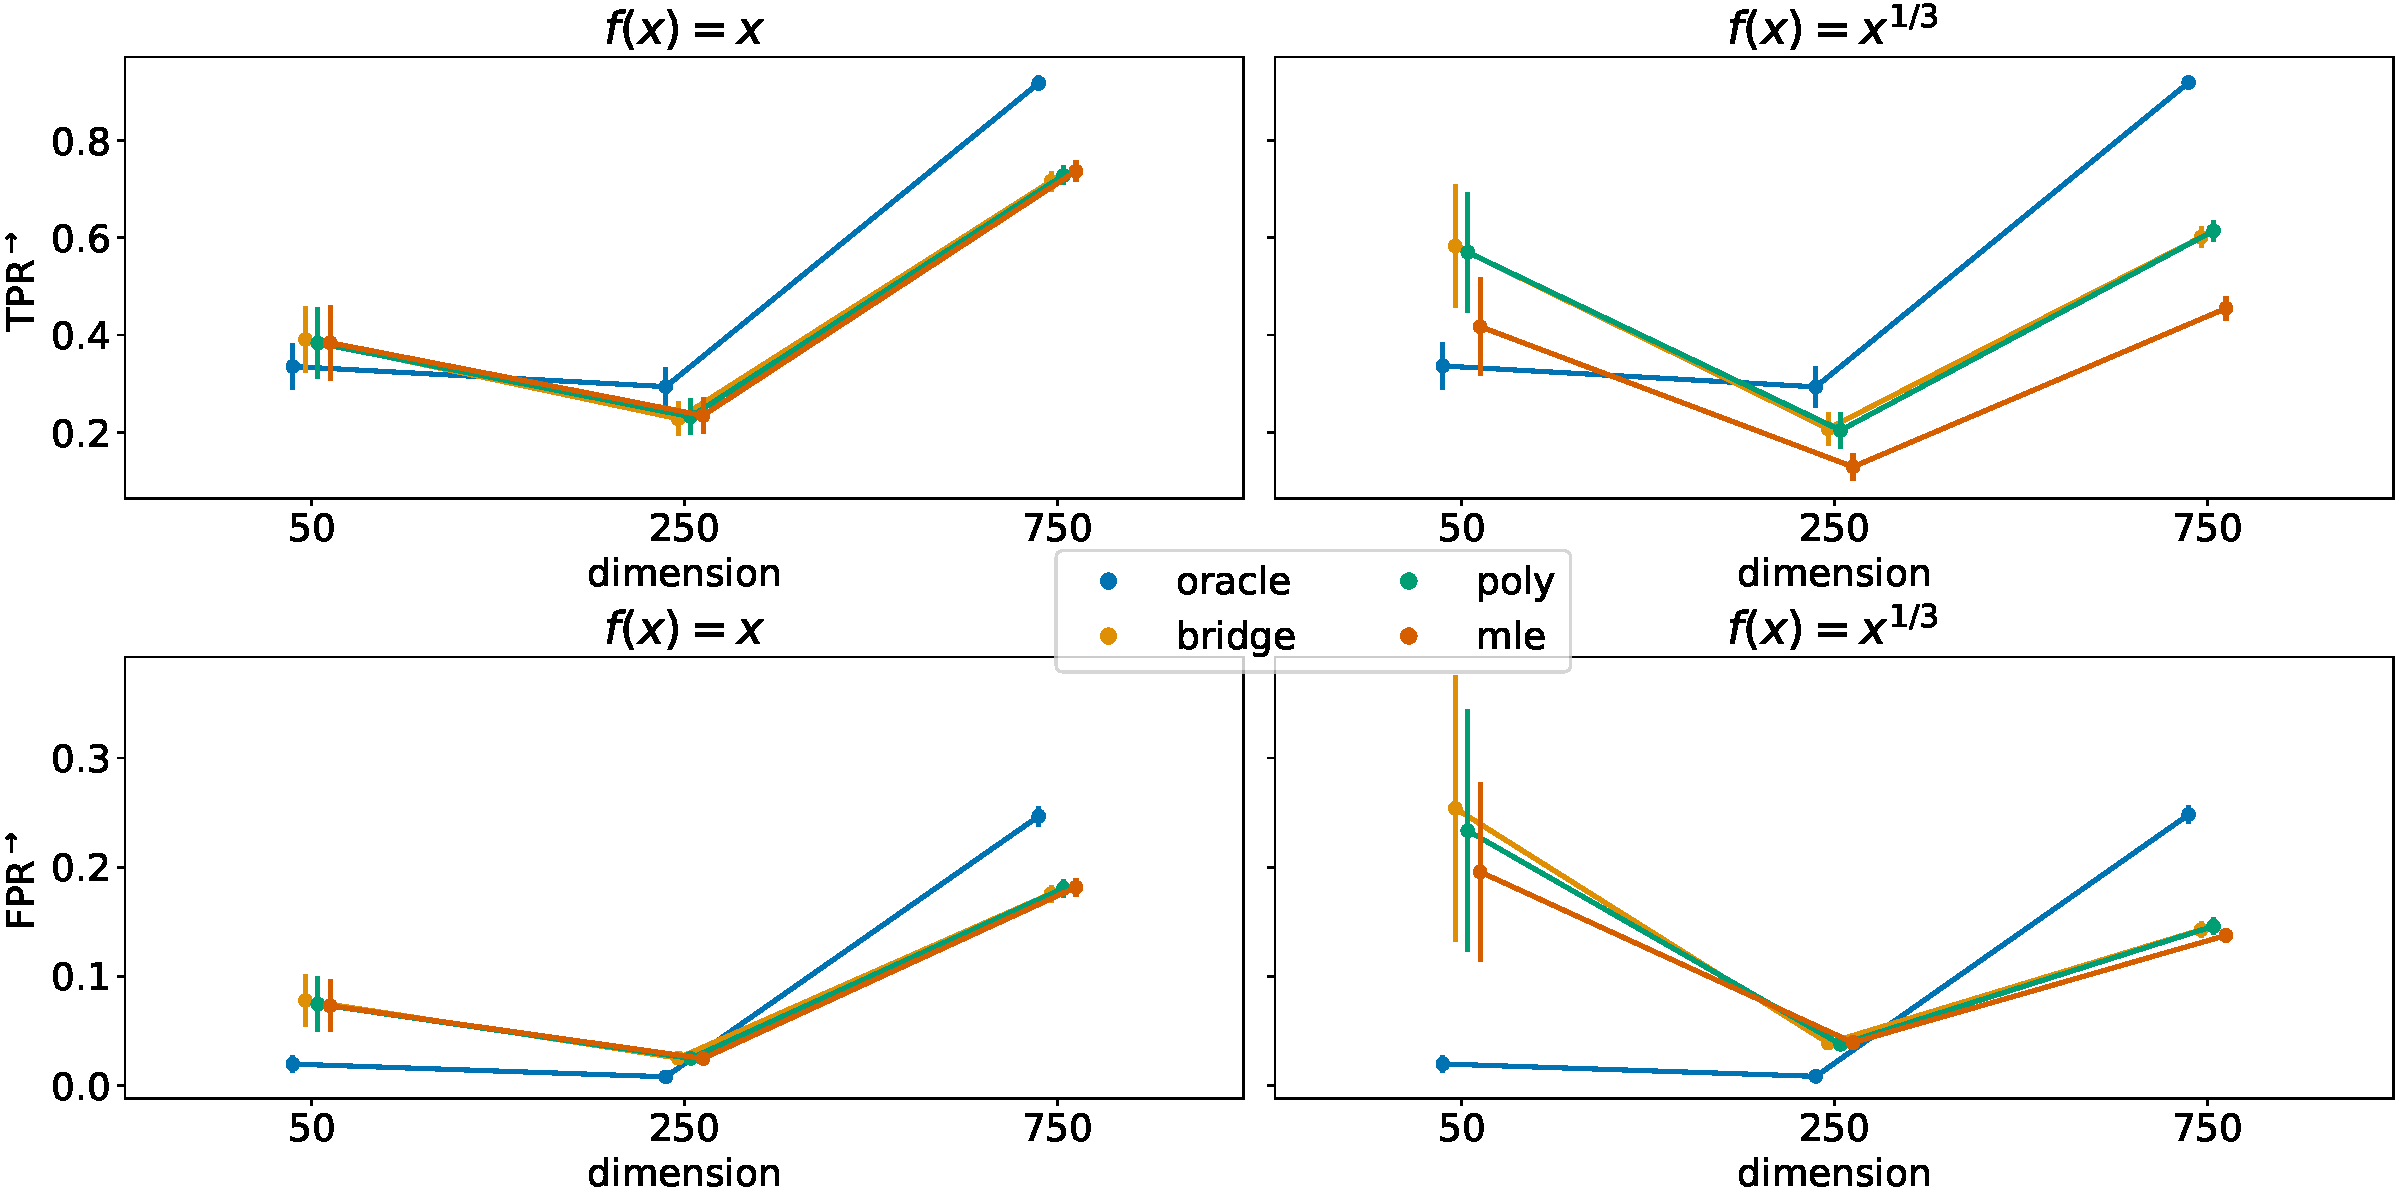
\includegraphics[width=\textwidth]{Figures/binary_fpr_tpr.pdf}
    \caption{Simulation results for the binary-continuous data setting based on \(100\) simulation runs. The left column corresponds to the latent Gaussian model, where the transformation function is the identity. The right colum depicts results for the LGCM with \(f_j(x) = x^{1/3}\) for all \(j\). The top and bottom rows report mean and standard deviation of the TPR and FPR along simulation runs, respectively. The y-axis labels have superscript arrows attached to indicate the direction of improvement: \(\rightarrow\) implies that larger values are better.}
    \label{fig:bench_tpr_fpr_binary}
\end{figure}


\begin{figure}
    \centering
    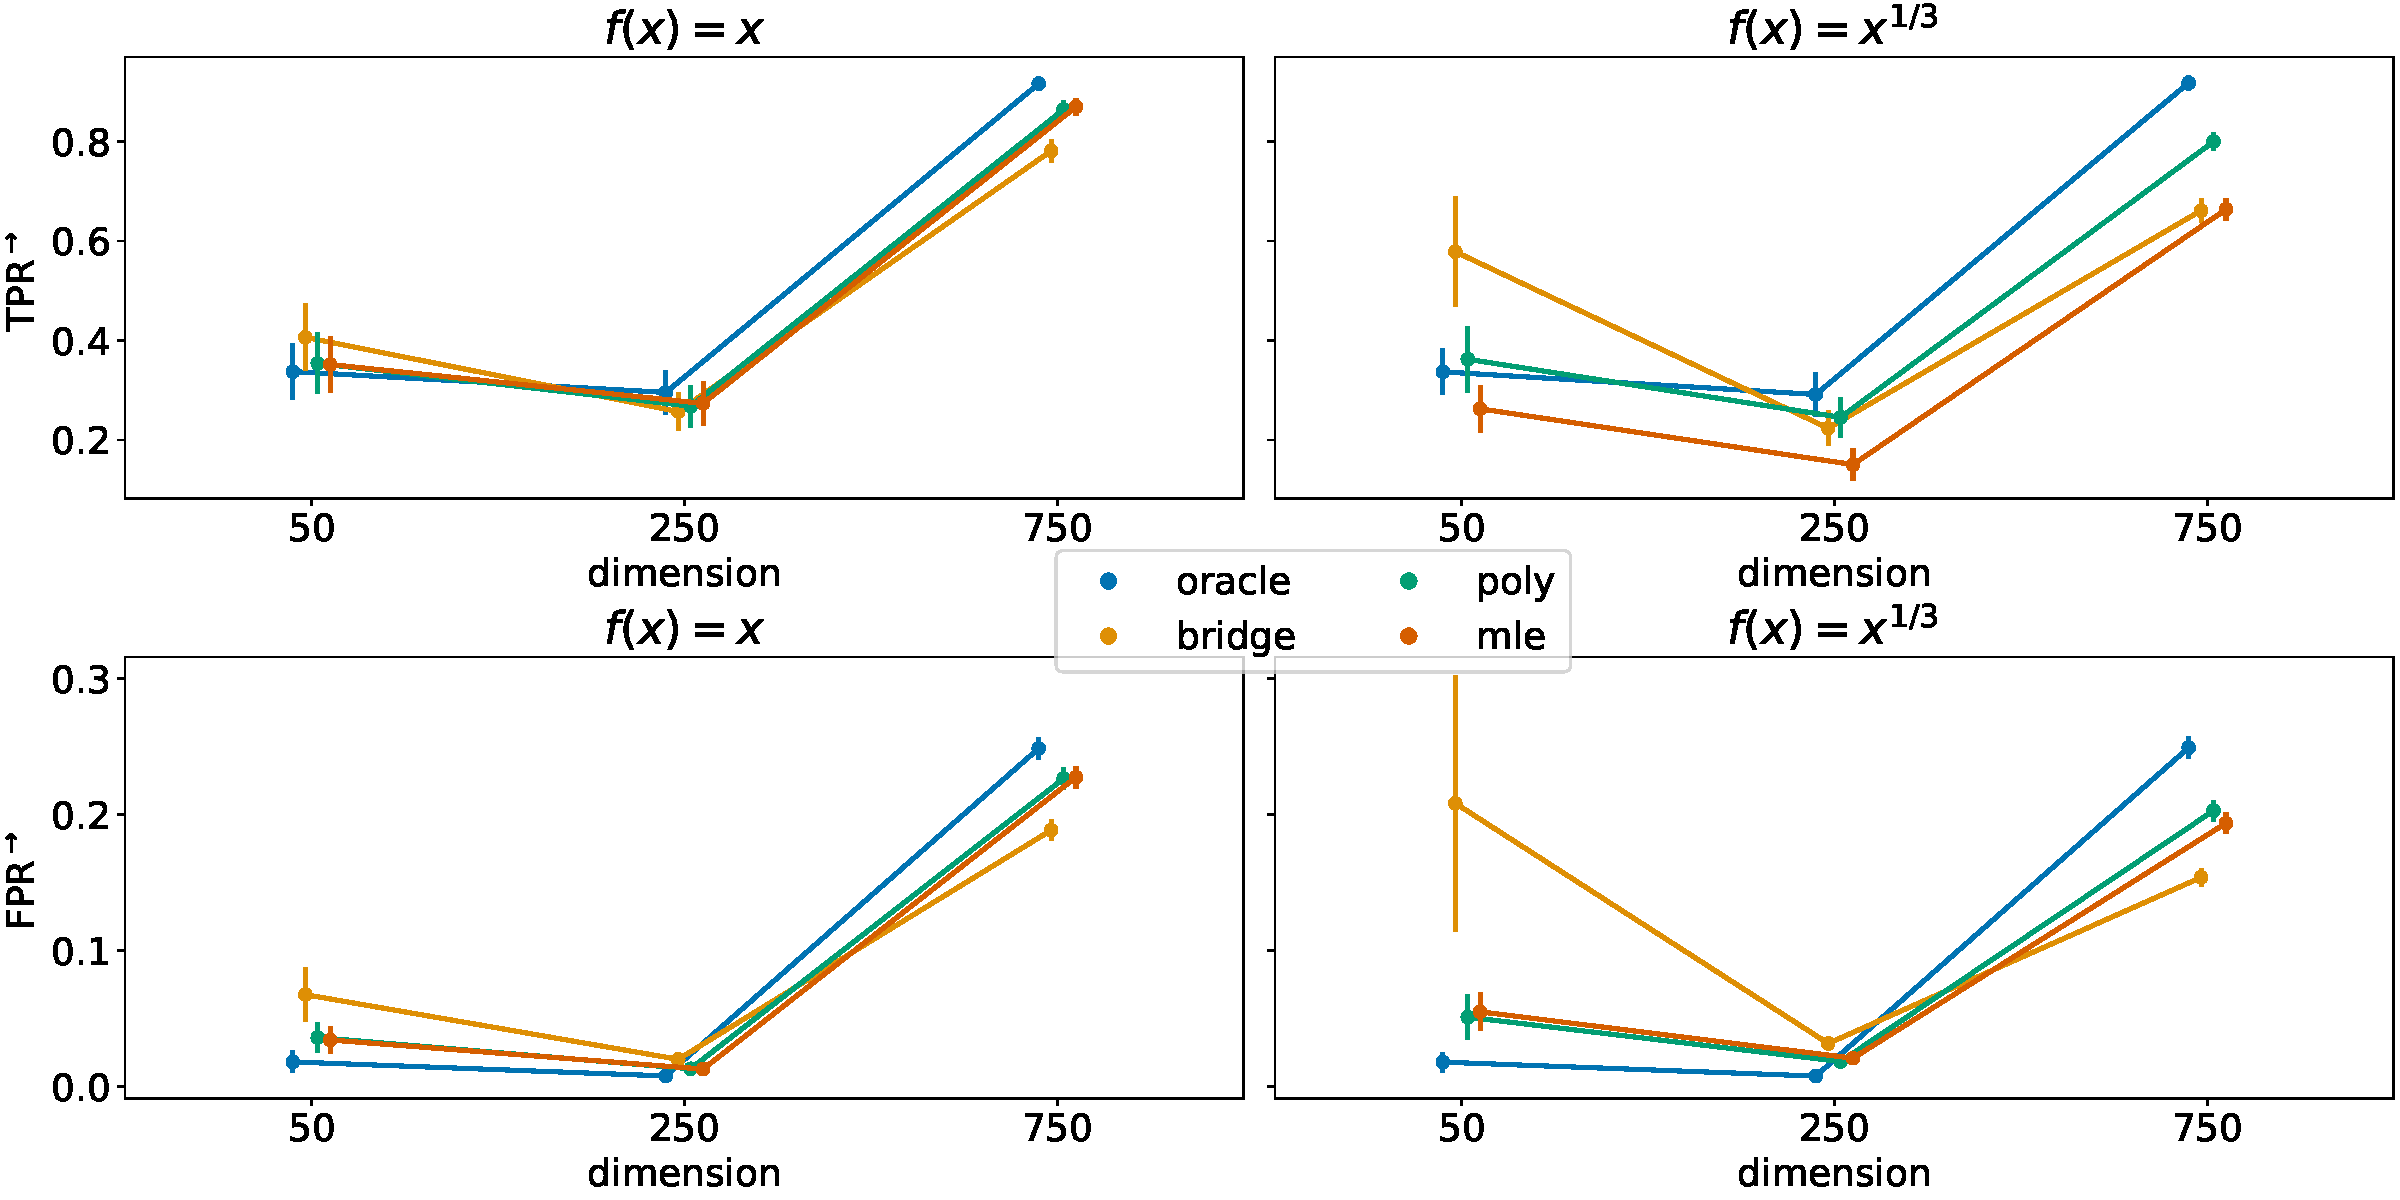
\includegraphics[width=\textwidth]{Figures/general_fpr_tpr.pdf}
    \caption{Simulation results for the general mixed data setting based on \(100\) simulation runs. The left column corresponds to the latent Gaussian model, where the transformation function is the identity. The right colum depicts results for the LGCM with \(f_j(x) = x^{1/3}\) for all \(j\). The top and bottom rows report mean and standard deviation of the TPR and FPR along simulation runs, respectively. The y-axis labels have superscript arrows attached to indicate the direction of improvement: \(\rightarrow\) implies that larger values are better.}
    \label{fig:bench_tpr_fpr_general}
\end{figure}


In the simulations carried out we start by constructing the true latent graph $\boldsymbol{\Omega}^*$. We set $\boldsymbol{\Omega}^*_{jj} = 1$ and $\boldsymbol{\Omega}_{jk}^* = s b_{jk}$ if $j\neq k$, where $s$ is the constant signal strength so as to assure positive definiteness. Furthermore, $b_{jk}$ are realizations of a Bernoulli random variable with corresponding success probability $p_{jk} = (2\pi)^{-1/2} \exp\big[\Norm{v_j - v_k}_2 / (2c) \big]$. In particular $v_j = (v_j^{(1)}, v_j^{(2)})$ are independent realizations of a bivariate uniform $[0,1]$ distribution and $c$ controls the sparsity of the graph. Throughout the experiments, $\hat{\Omega}$ is chosen by minimizing the eBIC according to the procedure outlined in Section 3.6 of the Manuscript %\ref{sec:precision_matrix} %
with $\theta = 0.1$ for the low and medium, $\theta = 0.5$ for the high dimensional graphs.

We set $s = 0.15$ and incrementally increase the dimensionality of each graph: $d= 50,250,750$ representing a transition from small to large scale graphs. We let $\boldsymbol{\Sigma}^* = (\boldsymbol{\Omega}^*)^{-1}$ rescaled such that all diagonal elements are equal to $1$. Equipped with $\Sigma^*$ we draw $n$ iid. samples from $\text{N}_d(\boldsymbol{0}, \boldsymbol{\Sigma}^*)$ obtaining realizations for the case of the latent Gaussian model. For the nonparanormal family, we sample from $\text{NPN}(\boldsymbol{0}, \boldsymbol{\Sigma}^*, f)$ where $f_j(x) = x^3$ for all $1 \leq j \leq d$.

In order to agree with the latent setup according to Definition 2.2
%\ref{def1}% 
let $\boldsymbol{X}_1$ be partitioned into equally sized collections of binary, ordinal and Poisson distributed random variables i.e. $\boldsymbol{X}_1 = (\boldsymbol{X}_1^{\text{bin}}, \boldsymbol{X}_1^{\text{ord}},\boldsymbol{X}_1^{\text{pois}})$ where the generative procedure is according to Eq. (1) of the main Manuscript. %\eqref{latent_ordered}. 

Recall, that for any continuous random variable $X$ with corresponding cumulative distribution function (CDF) $F_X$, $Y \coloneqq F_X(X)$ is a standard uniformly distributed random variable. Then, given $Y$ and with the aid of the inverse probability integral transform we can generate random samples from any cumulative distribution function \citep{Angus94}. Incidentally, this corresponds exactly to the relationship described in Eq. (1) of the main Manuscript.
%\eqref{latent_ordered}. %
For $\boldsymbol{X}_1^{\text{bin}}$ the aforementioned transformation is employed with success probability drawn from Uniform$[0.4,0.6]$ for $80\%$ of $\boldsymbol{X}_1^{\text{bin}}$. The remaining $20\%$ mimic unbalanced classes and success probability is drawn from Uniform$[0.05,0.1]$.

Regarding $\boldsymbol{X}_1^{\text{ord}}$, the inverse probability integral transform is used to generate samples from the multinomial distribution. To that end, the state space is drawn from Uniform$[3,10]$ and the corresponding probability of falling into one of these states is chosen to be proportional to the amount of states. Lastly, $\boldsymbol{X}_1^{\text{pois}}$ is generated with the inverse probability integral transform and the rate parameter set equal to $6$.

\subsection{Ternary mixed data results}

We now compare our method against \citeauthor{Quan18}'s (2018) generalization of the bridge function approach by \citet{Fan17} when a mix of ternary, binary, and continuous data is present. Recall that in this case $ \binom{2+2}{2} = 6$ bridge functions are needed.

The $(d,n)$-setup is analogous to the binary mixed case. Overall, when additionally to binary also ternary data is present both according to Table \ref{ternary_table} estimation error and graph recovery error reduce slightly. This is unsurprising as we now have more information about the underlying latent variables. Note that we expect the oracle $\hat{\Omega}$ to be roughly equivalent to the previous binary mixed case.

Starting with $\hat{\Omega}_{\text{MLE}}$ the pattern from the binary/continuous case continues to show in the ternary-binary mix: whenever $f(x)=x$ it generally performs best, in particular with respect to graph recovery.


    \begin{longtable}[c]{@{}*{6}{>{\arraybackslash}p{0.135\linewidth}}@{}}
    \caption{Ternary mixed data structure learning; Simulated data with $100$ simulation runs. Standard errors in brackets \label{ternary_table}}
    \\[-1.8ex]\hline 
    \hline \\[-1.8ex] 
    $d,n,f(x)$ && Oracle $\hat{\Omega}$ & ternary $\hat{\Omega}_{\tau}$ & $\hat{\Omega}_{\text{MLE}}$ & $\hat{\Omega}_r$ \\ 
    \hline \\[-1.8ex] 
    \multirow{8}{*}{$50,200,x$} & $\Norm{\hat{\Omega} - \Omega}_F$ & $2.860$ & $2.936$ & $2.935$ & $2.930$ \\ [-.25em]
    & & \footnotesize{($0.098$)} & \footnotesize{($0.105$)} & \footnotesize{($0.106$)} & \footnotesize{($0.109$)} \\ [.15em]
    & FPR & $0.016$ & $0.067$ & $0.071$ & $0.075$ \\ [-.25em] 
    & & \footnotesize{($0.005$)} & \footnotesize{($0.017$)} & \footnotesize{($0.021$)} & \footnotesize{($0.023$)} \\ [.15em] 
    & TPR & $0.340$ & $0.370$ & $0.381$ & $0.389$ \\ [-.25em]
    & & \footnotesize{($0.046$)} & \footnotesize{($0.061$)} & \footnotesize{($0.068$)} & \footnotesize{($0.070$)} \\ [.15em] 
    & AUC & $0.880$ & $0.758$ & $0.769$ & $0.764$ \\ [-.25em]
    & & \footnotesize{($0.013$)} & \footnotesize{($0.019$)} & \footnotesize{($0.019$)} & \footnotesize{($0.020$)} \\    [1em]
    %
    %
    \multirow{8}{*}{$50,200,x^3$} & $\Norm{\hat{\Omega} - \Omega}_F$ & $2.856$ & $2.942$ & $3.053$ & $2.935$ \\ [-.25em]
    & & \footnotesize{($0.116$)} & \footnotesize{($0.102$)} & \footnotesize{($0.098$)} & \footnotesize{($0.108$)} \\ [.15em]
    & FPR & $0.016$ & $0.068$ & $0.076$ & $0.075$ \\ [-.25em]
    & & \footnotesize{($0.007$)} & \footnotesize{($0.019$)} & \footnotesize{($0.020$)} & \footnotesize{($0.022$)} \\ [.15em]
    & TPR & $0.342$ & $0.372$ & $0.280$ & $0.391$ \\ [-.25em]
    & & \footnotesize{($0.051$)} & \footnotesize{($0.059$)} & \footnotesize{($0.051$)} & \footnotesize{($0.066$)} \\ [.15em]
    & AUC & $0.882$ & $0.759$ & $0.691$ & $0.768$ \\ [-.25em]
    & & \footnotesize{($0.015$)} & \footnotesize{($0.019$)} & \footnotesize{($0.020$)} & \footnotesize{($0.019$)} \\  [1em]
    %
    %
    \multirow{8}{*}{$250,200,x$} & $\Norm{\hat{\Omega} - \Omega}_F$ & $3.185$ & $3.742$ & $3.709$ & $3.711$ \\ [-.25em]
    & & \footnotesize{($0.097$)} & \footnotesize{($0.090$)} & \footnotesize{($0.089$)} & \footnotesize{($0.091$)} \\ [.15em] 
    & FPR & $0.006$ & $0.025$ & $0.024$ & $0.025$ \\ [-.25em]
    & & \footnotesize{($0.001$)} & \footnotesize{($0.003$)} & \footnotesize{($0.003$)} & \footnotesize{($0.003$)} \\ [.15em]
    & TPR & $0.308$ & $0.238$ & $0.237$ & $0.235$ \\ [-.25em]
    & & \footnotesize{($0.034$)} & \footnotesize{($0.033$)} & \footnotesize{($0.031$)} & \footnotesize{($0.030$)} \\ [.15em]
    & AUC & $0.884$ & $0.759$ & $0.773$ & $0.768$ \\ [-.25em]
    & & \footnotesize{($0.014$)} & \footnotesize{($0.018$)} & \footnotesize{($0.018$)} & \footnotesize{($0.018$)} \\   [1em]
    %
    %
    \multirow{8}{*}{$250,200,x^3$} & $\Norm{\hat{\Omega} - \Omega}_F$ & $3.199$ & $3.757$ & $3.894$ & $3.724$ \\ [-.25em]
    & & \footnotesize{($0.096$)} & \footnotesize{($0.096$)} & \footnotesize{($0.096$)} & \footnotesize{($0.087$)} \\ [.15em]
    & FPR & $0.006$ & $0.025$ & $0.026$ & $0.025$ \\ [-.25em]
    & & \footnotesize{($0.001$)} & \footnotesize{($0.003$)} & \footnotesize{($0.003$)} & \footnotesize{($0.003$)} \\ [.15em]
    & TPR & $0.302$ & $0.239$ & $0.143$ & $0.237$ \\ [-.25em]
    & & \footnotesize{($0.034$)} & \footnotesize{($0.032$)} & \footnotesize{($0.027$)} & \footnotesize{($0.032$)} \\ [.15em] 
    & AUC & $0.882$ & $0.759$ & $0.691$ & $0.767$ \\ [-.25em]
    & & \footnotesize{($0.012$)} & \footnotesize{($0.016$)} & \footnotesize{($0.016$)} & \footnotesize{($0.015$)} \\  [1em]
    %
    %
    \multirow{8}{*}{$750,300,x$} & $\Norm{\hat{\Omega} - \Omega}_F$ & $11.181$ & $10.830$ & $10.640$ & $10.659$ \\ [-.25em] 
    & & \footnotesize{($0.134$)} & \footnotesize{($0.129$)} & \footnotesize{($0.122$)} & \footnotesize{($0.118$)} \\ [.15em]
    & FPR & $0.256$ & $0.179$ & $0.180$ & $0.179$ \\ [-.25em]
    & & \footnotesize{($0.006$)} & \footnotesize{($0.006$)} & \footnotesize{($0.006$)} & \footnotesize{($0.005$)} \\ [.15em] 
    & TPR & $0.937$ & $0.723$ & $0.744$ & $0.736$ \\ [-.25em]
    & & \footnotesize{($0.009$)} & \footnotesize{($0.016$)} & \footnotesize{($0.017$)} & \footnotesize{($0.016$)} \\ [.15em]
    & AUC & $0.939$ & $0.820$ & $0.831$ & $0.828$ \\ [-.25em]
    & & \footnotesize{($0.006$)} & \footnotesize{($0.009$)} & \footnotesize{($0.009$)} & \footnotesize{($0.009$)} \\ 
    [1em]
    \multirow{8}{*}{$750,300,x^3$} & $\Norm{\hat{\Omega} - \Omega}_F$ & $11.196$ & $10.838$ & $11.250$ & $10.646$ \\ [-.25em]
    & & \footnotesize{($0.130$)} & \footnotesize{($0.129$)} & \footnotesize{($0.130$)} & \footnotesize{($0.137$)} \\ [.15em] 
    & FPR & $0.256$ & $0.180$ & $0.173$ & $0.179$ \\ [-.25em]
    & & \footnotesize{($0.006$)} & \footnotesize{($0.006$)} & \footnotesize{($0.006$)} & \footnotesize{($0.006$)} \\ [.15em]
    & TPR & $0.937$ & $0.724$ & $0.590$ & $0.737$ \\ [-.25em]
    & & \footnotesize{($0.009$)} & \footnotesize{($0.016$)} & \footnotesize{($0.020$)} & \footnotesize{($0.016$)} \\ [.15em]
    & AUC & $0.939$ & $0.820$ & $0.743$ & $0.828$ \\ [-.25em]
    & & \footnotesize{($0.006$)} & \footnotesize{($0.008$)} & \footnotesize{($0.011$)} & \footnotesize{($0.009$)} \\ 
    \hline \\[-1.8ex] 
    \end{longtable} 


However, when $f_j(x)=x^3$ performance drops notably which again is driven not by an increased FPR but by a decreased TPR.
Again, results for $\hat{\boldsymbol\Omega}_\tau$ and $\hat{\boldsymbol\Omega}_r$ are similar although there appears to be a pattern in the sense of some evidence of smaller estimation error and better graph recovery all throughout the experiments by using our estimator $\hat{\boldsymbol\Omega}_r$.

Overall, no performance reduction neither in terms of estimation error nor in graph recovery can be detected when comparing $\hat{\boldsymbol\Omega}_r$ to the ternary $\hat{\boldsymbol\Omega}_\tau$. In fact, the opposite is the case. Consequently, in both special cases of Definition 2.2 %\ref{def1}%
-- the binary and the ternary mixed scheme --
these results support the use of the polychoric and polyserial estimation strategies as a simpler and more general approach as compared with constructing bridge functions for every combination of variables and their state spaces.



%%%%%%%%%%%%%%%%%%%%%%%%%%%%%%%%%%%%%%%%%%%%%%%%%%%%%%%%%%%%%%%%%%%%%%%
%\clearpage
%\newpage
%\pagebreak

\section{Variable Description for real world data application}

Table \ref{tab:var_descr} gives an overview over the variables present in the UK Biobank data set.

    \begin{longtable}[c]{lp{8cm}}
    \caption{Variable description of the real world application \label{tab:var_descr}}\\    %%%%<===
    \\[-1.8ex]\hline 
    \hline \\[-1.8ex] 
    Variable Name 	&	Description	\\ 
    \hline \\[-1.8ex] 
        age	&	age in. years in 2020	\\
        waist circ.	&	waist circumference in cm	\\
        height	&	standing in height in cm 	\\
        first illn.	&	age at which illness first occurred 	\\
        first surg. 	&	age at which operation was done first	\\
        pulse rate	&	pulse rate measured in bpm 	\\
        deprev. idx	&	Townsend deprivation index at recruitment	\\
        dur. walks	&	duration of walks in minutes per day	\\
        dur. mod. act. 	&	duration of moderate activity in minutes per day	\\
        dbp	&	diastolic blood pressure in mmHg	\\
        sbp	&	systolic blood pressure in mmHg	\\
        BMI	&	in kg/m2	\\
        weigth	&	in kg	\\
        b.f. perc.	&	body fat percentage in \%	\\
        walking	&	number of days per week walked 10+ minutes 	\\
        mod. phys. act.	&	number of days per week of moderate physical activity  10+ minutes 	\\
        vig. phys. act.	&	number of days per week of vigorous physical activity 10+ minutes 	\\
        cheese	&	answer to ``How often do you eat cheese per week?" 	\\
        stair climb.	&	answer to "At home, during the last 4 weeks, about how many times a DAY do you climb a flight of stairs? (approx 10 steps)" 	\\
        curr. smoking	&	categorial, "Do you smoke tobacco now?" (yes, no, occasionally)	\\
        past smoking	&	categorial, "How often did you smoke tobacco?" (never, once/twice, occasionally, on most days)	\\
        diet var.	&	categorial, "Does your diet change?" (never, sometimes, often)	\\
        alc. freq.	&	categorial, "How often do you drink alcohol?" (never, special occasions only, 1-3 per month, 1-2 per week, 3-4 per week, almost daily)	\\
        alc. var.	&	categorial, "Compared to 10 years ago, do you drink?" (more, about the same, less)	\\
        sex	&	binary indicator with 0=female, 1=male	\\
        hypertension	&	hypertension, binary indicator with 0=no, 1=yes	\\
        angina	&	angina, binary indicator with 0=no, 1=yes	\\
        heart attack	&	heart attack, binary indicator with 0=no, 1=yes	\\
        stroke	&	stroke, binary indicator with 0=no, 1=yes	\\
        dvt	&	deep venous thrombosis, binary indicator with 0=no, 1=yes	\\
        asthma	&	asthma, binary indicator with 0=no, 1=yes	\\
        chr. bronch.	&	emphysema/chronic bronchitis,  binary indicator with 0=no, 1=yes	\\
        gord	&	gastro-oesophageal reflux/gastric reflux, binary indicator with 0=no, 1=yes	\\
        ibs	&	irritable bowel syndrome, binary indicator with 0=no, 1=yes	\\
        gall stones	&	cholelithiasis/gall stones, binary indicator with 0=no, 1=yes	\\
        kidn./bladder stone 	&	kidney stone/ureter stone/bladder stone, binary indicator with 0=no, 1=yes	\\
        diabetes	&	diabetes, binary indicator with 0=no, 1=yes	\\
        diabtes 2	&	type 2 diabetes, binary indicator with 0=no, 1=yes	\\
        myxoedema	&	hypothyroidism/myxoedema, binary indicator with 0=no, 1=yes	\\
        migraine	&	migraine, binary indicator with 0=no, 1=yes	\\
        glaucoma	&	glaucoma, binary indicator with 0=no, 1=yes	\\
        cataract	&	cataract, binary indicator with 0=no, 1=yes	\\
        depression	&	depression, binary indicator with 0=no, 1=yes	\\
        panic attacks	&	anxiety/panic attacks, binary indicator with 0=no, 1=yes	\\
        back probl. 	&	back problems, binary indicator with 0=no, 1=yes	\\
        osteoporosis	&	osteoporosis, binary indicator with 0=no, 1=yes	\\
        spine arthr.	&	spine arthritis/spondylitis, binary indicator with 0=no, 1=yes	\\
        slipped disc	&	prolapsed disc/slipped disc, binary indicator with 0=no, 1=yes	\\
        anaemia 	&	iron deficiency anaemia, binary indicator with 0=no, 1=yes	\\
        ut. fibroids	&	uterine fibroids, binary indicator with 0=no, 1=yes	\\
        allerg. rhinitis	&	heyfever/allergic rhinitis, binary indicator with 0=no, 1=yes	\\
        enlarged prost.	&	enlarged prostate, binary indicator with 0=no, 1=yes	\\
        pneumonia	&	pneumonia, binary indicator with 0=no, 1=yes	\\
        endometr.	&	endometriosis, binary indicator with 0=no, 1=yes	\\
        ear disor.	&	ear/vestibular disorder, binary indicator with 0=no, 1=yes	\\
        headaches	&	headaches (not migraine), binary indicator with 0=no, 1=yes	\\
        ecz./dermat.	&	eczema/dermatitis, binary indicator with 0=no, 1=yes	\\
        psoriasis	&	psoriasis, binary indicator with 0=no, 1=yes	\\
        div. disease	&	diverticular disease/diverticulitis, binary indicator with 0=no, 1=yes	\\
        osteoarthr.	&	osteoarthritis, binary indicator with 0=no, 1=yes	\\
        gout	&	gout, binary indicator with 0=no, 1=yes	\\
        high chol.	&	high cholesterol, binary indicator with 0=no, 1=yes	\\
        hiat. hern.	&	hiatus hernia, binary indicator with 0=no, 1=yes	\\
        sciatica	&	sciatica, binary indicator with 0=no, 1=yes	\\
        appendic.	&	appendicitis, binary indicator with 0=no, 1=yes	\\
        back pain	&	back pain, binary indicator with 0=no, 1=yes	\\
        arthritis	&	arthritis (nos), binary indicator with 0=no, 1=yes	\\
        measles	&	measles/morbillivirus, binary indicator with 0=no, 1=yes	\\
        chickpox	&	chickenpox, binary indicator with 0=no, 1=yes	\\
        tonsillitis	&	tonsillitis, binary indicator with 0=no, 1=yes	\\
        ptca	&	coronary angioplasty (ptca)+/-stent, binary indicator with 0=no, 1=yes	\\
        ear surg.	&	ear surgery, binary indicator with 0=no, 1=yes	\\
        sinus surg.	&	nasal/sinus,nose surgery, binary indicator with 0=no, 1=yes	\\
        vasectomy	&	vasectomy, binary indicator with 0=no, 1=yes	\\
        soft tiss. surg.	&	mucsle/soft tissue surgery, binary indicator with 0=no, 1=yes	\\
        hip repl.	&	hip replacement/revision, binary indicator with 0=no, 1=yes	\\
        knee repl.	&	knee replacement/revision, binary indicator with 0=no, 1=yes	\\
        spine surg.	&	spine or back surgery, binary indicator with 0=no, 1=yes	\\
        bil. ooph.	&	bilateral oophorectomy, binary indicator with 0=no, 1=yes	\\
        hysterect.	&	hysterectomy, binary indicator with 0=no, 1=yes	\\
        steril.	&	sterilisation, binary indicator with 0=no, 1=yes	\\
        lumpect.	&	lumpectomy, binary indicator with 0=no, 1=yes	\\
        ing. hernia rep.	&	inguinal/femoral hernia repair, binary indicator with 0=no, 1=yes	\\
        umb. hernia rep.	&	umbilical hernia repair, binary indicator with 0=no, 1=yes	\\
        cataract extr.	&	catarct extraction/lens implant, binary indicator with 0=no, 1=yes	\\
        red./fix. bone frac.	&	reduction or fixationof bone fracture, binary indicator with 0=no, 1=yes	\\
         cholecystect. 	&	cholecystectomy/gall bladder removal, binary indicator with 0=no, 1=yes	\\
        appendicect.	&	appendicectomy, binary indicator with 0=no, 1=yes	\\
        c-sec.	&	caesarian section, binary indicator with 0=no, 1=yes	\\
        tonsillest.	&	tonsillectomy, binary indicator with 0=no, 1=yes	\\
        var. vein surg.	&	varicose vein surgery, binary indicator with 0=no, 1=yes	\\
        wisd. teeth surg.	&	wisdom teeth surgery, binary indicator with 0=no, 1=yes	\\
        piles surg.	&	haemorroidectomy/piles surgery/banding of piles, binary indicator with 0=no, 1=yes	\\
        male circ.	&	male circumcision, binary indicator with 0=no, 1=yes	\\
        squint corr.	&	squint correction, binary indicator with 0=no, 1=yes	\\
        arthrosc.	&	arthroscopy (nos), binary indicator with 0=no, 1=yes	\\
        foot surg.	&	foot surgery, binary indicator with 0=no, 1=yes	\\
        knee surg.	&	knee surgery (not replacement), binary indicator with 0=no, 1=yes	\\
        shoulder surg.	&	shoulder surgery, binary indicator with 0=no, 1=yes	\\
        car. tunn. surg.	&	carpal tunnel surgery, binary indicator with 0=no, 1=yes	\\
        valg. surg.	&	bunion/hallus valgus surgery, binary indicator with 0=no, 1=yes	\\
        rem. mole	&	removal of mole/skin lesion, binary indicator with 0=no, 1=yes	\\
        ov. cyst. rem.	&	ovarian cyst removal/surgery, binary indicator with 0=no, 1=yes	\\
        d+c	&	dilatation and curettage, binary indicator with 0=no, 1=yes	\\
        cone biops.	&	cone biopsy, binary indicator with 0=no, 1=yes	\\
        endosc.	&	endoscopy/gastroscopy, binary indicator with 0=no, 1=yes	\\
        colonosc.	&	colonoscopy/sigmoidoscopy, binary indicator with 0=no, 1=yes	\\
        laparosc.	&	laparoscopy, binary indicator with 0=no, 1=yes	\\
        rhinoplast.	&	rhinoplasty/nose surgery, binary indicator with 0=no, 1=yes	\\
        tonsil surg.	&	tonsillectomy/tonsil surgery, binary indicator with 0=no, 1=yes	\\
        ing. hern. rep.	&	inguinal hernia repair, binary indicator with 0=no, 1=yes	\\
        illn. ind. diet	&	Major dietary changes in the last 5 years because of illness, binary indicator with 0=no, 1=yes	\\
        diet change	&	Major dietary changes in the last 5 years  because of other reason, binary indicator with 0=no, 1=yes	\\
        ethn. Mixed	&	Ethnicity - mixed, binary indicator with 0=no, 1=yes	\\
        ethn. Asian	&	Ethnicity - Asian, binary indicator with 0=no, 1=yes	\\
        ethn. Black	&	Ethnicity - Black, binary indicator with 0=no, 1=yes	\\
        no eggs	&	Never eat eggs or foods containing eggs, binary indicator with 0=no, 1=yes	\\
        no dairy	&	Never dairy products, binary indicator with 0=no, 1=yes	\\
        no wheat	&	Never eat wheat, binary indicator with 0=no, 1=yes	\\
        no sugar	&	Never eat sugar or foods/drinks containing sugar, binary indicator with 0=no, 1=yes	\\
        walk. f. pleas.	&	Types of physical activity in last 4 weeks - walking for pleasure, binary indicator with 0=no, 1=yes	\\
        exercises	&	Types of physical activity in last 4 weeks - other exercises (swimming, bowling etc.), binary indicator with 0=no, 1=yes	\\
        stren. Sports	&	Types of physical activity in last 4 weeks -  strenuous sports, binary indicator with 0=no, 1=yes	\\
        Covid-19 severity	&	Covid-19 severity, binary indicator with 0=mild outcome and 1=severe outcome	\\
    \hline
\end{longtable}


\begin{comment}


\newpage

\section{Data Simulation Function}
\textbf{Input of \texttt{simulate.mixed.data}:}
\begin{itemize}
    \item Number of observations \texttt{N}
    \item Vector \texttt{pfrac=c(gauss,poiss,bin,negbin,multinom)} with number of normally,  poisson,  binary, negative binomial and multinomial variables
    \item \texttt{Omega}: (opt.) precision matrix of the underlying latent Gaussian variables
    \item Seed \texttt{seed}
    \item Sparsity level \texttt{sparsity}
    \item \texttt{lambda}: (opt) vector of length \texttt{poiss} containing $\lambda$'s
    \item  \texttt{pbin}: (opt) vector of length \texttt{bin} containing the probabilities of success
    \item  \texttt{negbin}: (opt) list with first element being a vector of number of successes and the second element being a vector of probabilities of success
    \item  \texttt{multinom}: (opt) list of length \texttt{multinom} of vectors containing prob breaks
\end{itemize}
\textbf{Output of \texttt{simulate.mixed.data}:}
\begin{itemize}
    \item  data matrix \texttt{Xdata}
    \item adjacency matrix \texttt{A}
    \item underlying latent Gaussian data matrix \texttt{X}
    \item  the true precision matrix \texttt{K}
\end{itemize}


\subsection*{Data Simulation Process}
\begin{itemize}
    \item[\textbf{1}.] Draw $\texttt{X}\sim N(\mu,K^{-1})$ with $\texttt{X}$ being of dimension $N \times $\texttt{ptotal} with

        \texttt{ptotal} =\texttt{gauss}+\texttt{poiss}+\texttt{bin}+\texttt{negbin}+\texttt{multinom} and where $\mu \sim N(0,1)$  and $K$ being sparse with sparsity level \texttt{spars}

    \item[\textbf{2}.] Every non-zero entry $k \in K$ other than the main diagonal corresponds to a entry of 1 in matrix \texttt{A}

    \item[\textbf{3}.] \texttt{X} is now being split into \texttt{Xgauss} ($N\times \texttt{gauss}$), \texttt{Xpoiss} ($N\times \texttt{poiss}$), \texttt{Xbin} ($N\times \texttt{bin}$), \texttt{Xnegbin} ($N\times \texttt{negbin}$) and \texttt{Xmultinom} ($N\times \texttt{multinom}$)

    \item[\textbf{4}.] We then transform  \texttt{Xpoiss},\texttt{Xbin},  \texttt{Xnegbin},\texttt{Xmultinom} into their corresponding variable type:
        \begin{itemize}
            \item[ \texttt{Xpoiss}::]  qpois(pnorm(scale(\texttt{Xpoiss})), lambda=lambda):
                \begin{itemize}
                    \item[i] lambda=abs(rnorm(\texttt{poiss}))*5 (default)
                    \item[] or
                    \item[ii] lambda=\texttt{lambda} being a vector of length \texttt{poiss} set by the user
                \end{itemize}


            \item[\texttt{Xbin}::]  qbinom(pnorm(scale(\texttt{Xbin})),  size = 1,  prob = prob):
                \begin{itemize}
                    \item[i] prob=runif(\texttt{bin},0.2,0.8) (default)
                    \item[] or
                    \item[ii] prob=\texttt{pbin} being a vector of probabilities of  length \texttt{bin} set by the user
                \end{itemize}

            \item[\texttt{Xnegbin}::] qnbinom(pnorm(scale(\texttt{Xnegbin})),  size=negbin{\_}size,  prob=negbin{\_}prob):
                \begin{itemize}
                    \item[i] negbin{\_}size= round(runif(\texttt{negbin},0,1)*5) (default)
                    \item[i] negbin{\_}prob= runif(\texttt{negbin},0.2,0.8) (default)
                    \item[] or
                    \item[ii] negbin{\_}size= \texttt{negbin}[1] vector of length \texttt{negbin} specified by user
                    \item[ii] negbin{\_}prob= \texttt{negbin}[2] vector of length \texttt{negbin} specified by user
                \end{itemize}


            \item[\texttt{Xmultinom}::]  cut(pnorm(scale(\texttt{Xmultinom})),  breaks=cum.mat):
                \begin{itemize}
                    \item[i] cum.mat=c(0,cumsum(sort(

                        runif(round(runif(1,0,2)*5)))/sum(runif(round(runif(1,0,2)*5)))))
                    \item[] or
                    \item[ii] cum.mat =\texttt{multinom}  being \texttt{multinom} dimensional list of vectors containing the breaks specified by user
                \end{itemize}
        \end{itemize}


    \item[\textbf{5}.] After the previous step we create  \texttt{Xdata} by concatenating the transformed parts of \texttt{X} such that  \texttt{Xdata}=\texttt{cbind}(\texttt{Xgauss},\texttt{Xpoiss},\texttt{Xbin},  \texttt{Xnegbin},\texttt{Xmultinom})

\end{itemize}


%\clearpage\newpage


%%%%%%%%%%%%%%%%%
\section{Additional Simulation Results}


\begin{figure}
    \hspace*{-2ex}
    \hfill
    \subfigure[]{\includegraphics[width=0.32\textwidth]{Figures/ROCs_based_on_data_set_B_large.pdf}}
    \hspace*{-2ex}
    \hfill\subfigure[]{\includegraphics[width=0.32\textwidth]{Figures/ROCs_based_on_data_set_B_largecorr_largeN.pdf}}
    \hspace*{-2ex}
    \hfill\subfigure[]{\includegraphics[width=0.32\textwidth]{Figures/ROCs_based_on_data_set_B_01_large.pdf}}
    \label{fig:ROCs_based_on_data_set_B_large}
    \caption{ROCs based on data set B with sample size increased four times. On the left, (a), using empirical parameters, in the middle, (b), using empirical parameters but only evaluating partial correlations with absolute value larger than 0.1 and on the right, (c), using empirical parameters with sparser, thresholded precision as input.}
\end{figure}



\begin{figure}
    \hspace*{-2ex}
    \hfill\subfigure[]{\includegraphics[width=0.32\textwidth]{Figures/ROCs_based_on_data_set_D.pdf}}
    \hfill\subfigure[]{\includegraphics[width=0.32\textwidth]{Figures/ROCs_based_on_data_set_D_largecorr.pdf}}
    \hspace*{-2ex}
    \hfill\subfigure[]{\includegraphics[width=0.32\textwidth]{Figures/ROCs_based_on_data_set_D_01.pdf}}
    \label{fig:ROCs_based_on_data_set_D}
    \caption{ROCs based on data set D. On the left, (a), using empirical parameters, in the middle, (b), using empirical parameters but only evaluating partial correlations with absolute value larger than 0.1 and on the right, (c), using empirical parameters with sparser, thresholded precision as input.}
\end{figure}



\begin{figure}
    \hspace*{-2ex}
    \hfill\subfigure[]{\includegraphics[width=0.32\textwidth]{Figures/ROCs_based_on_data_set_D_large.pdf}}
    \hfill\subfigure[]{\includegraphics[width=0.32\textwidth]{Figures/ROCs_based_on_data_set_D_largecorr_largeN.pdf}}
    \hspace*{-2ex}
    \hfill\subfigure[]{\includegraphics[width=0.32\textwidth]{Figures/ROCs_based_on_data_set_D_01_large.pdf}}
    \label{fig:ROCs_based_on_data_set_D_large}
    \caption{ROCs based on data set D with sample size increased four times. On the left, (a), using empirical parameters, in the middle, (b), using empirical parameters but only evaluating partial correlations with absolute value larger than 0.1 and on the right, (c), using empirical parameters with sparser, thresholded precision as input.}
\end{figure}



\end{comment}

%\clearpage\newpage


%%%%%%%%%%%%%%%%%

\section{Additional Empirical Results}

\subsection*{Empirical Results for Subset B}
Figures \ref{fig:corrplot_admat_B} and \ref{fig:corrplot_omega_B} exemplify additional empirical results for subset B.

\begin{figure}[ht]
    \centering
    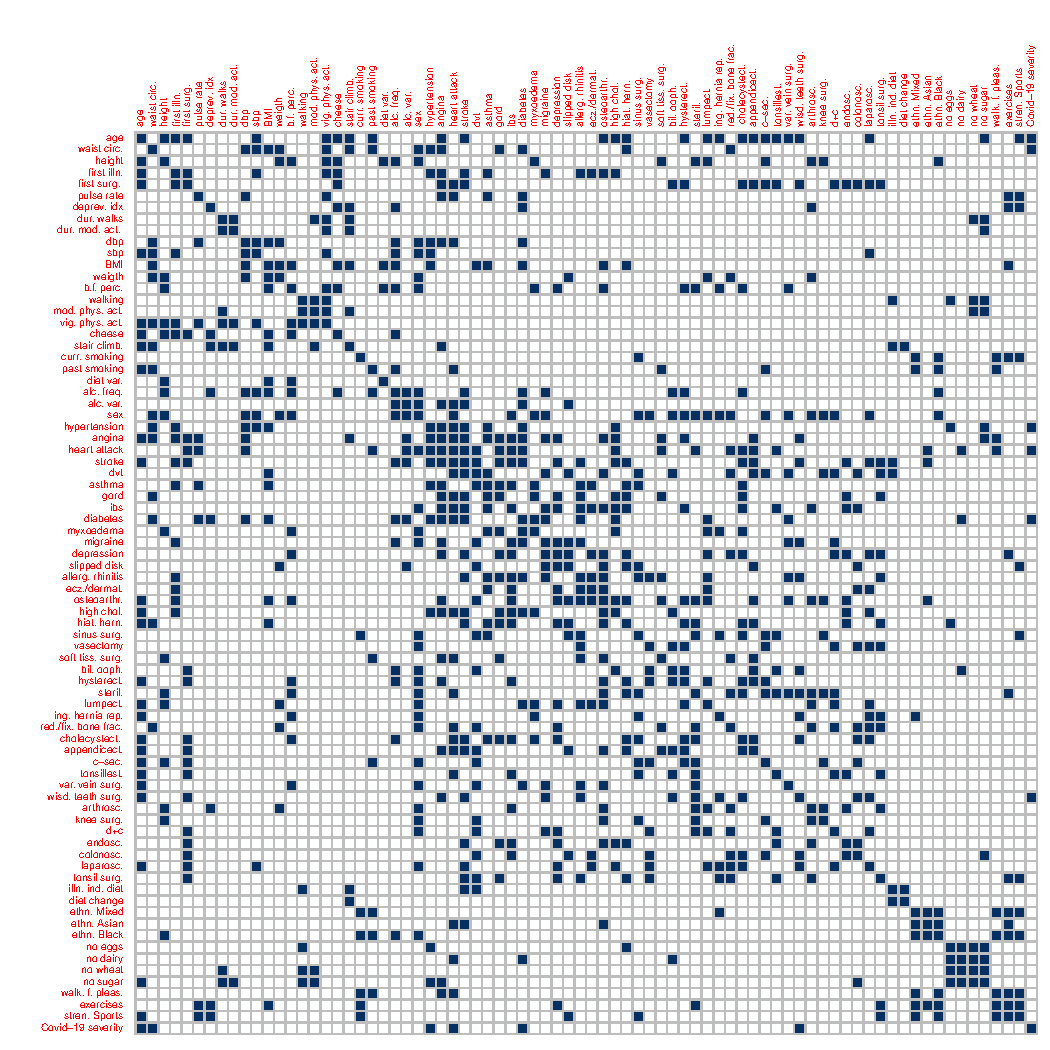
\includegraphics[width=1.0\textwidth]{Figures/corrplot_admat_B.pdf}
    \caption{Plot of the estimated adjacency matrix of data set B.}
    \label{fig:corrplot_admat_B}
\end{figure}

\begin{figure}
    \centering
    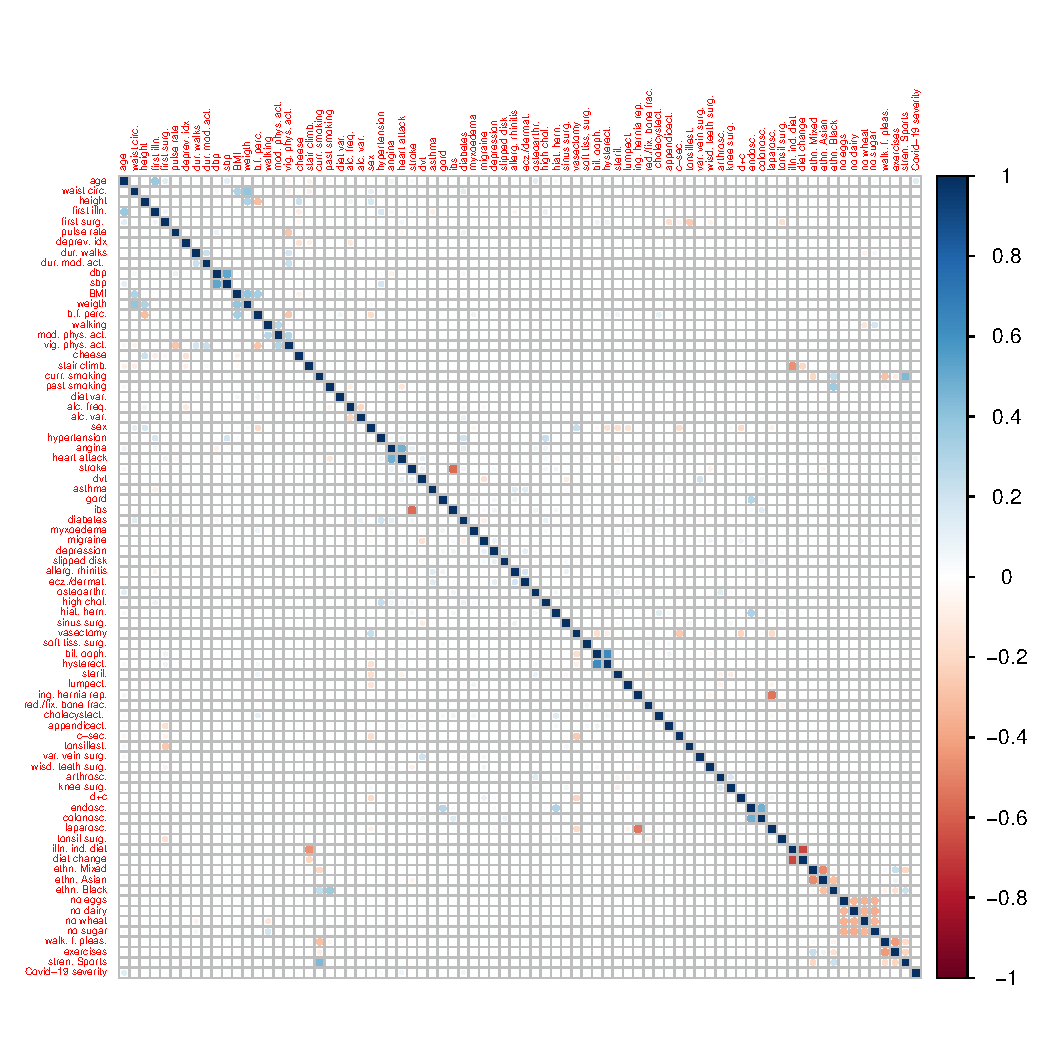
\includegraphics[width=1.0\textwidth]{Figures/corrplot_omega_B.pdf}
    \caption{Plot of the estimated precision matrix of data set B.}
    \label{fig:corrplot_omega_B}
\end{figure}


%\newpage
\subsection*{Empirical Results for Subset C}

Figures \ref{fig:corrplot_admat_C} and \ref{fig:corrplot_omega_C} exemplify additional empirical results for subset C.

\begin{figure}[ht]
    \centering
    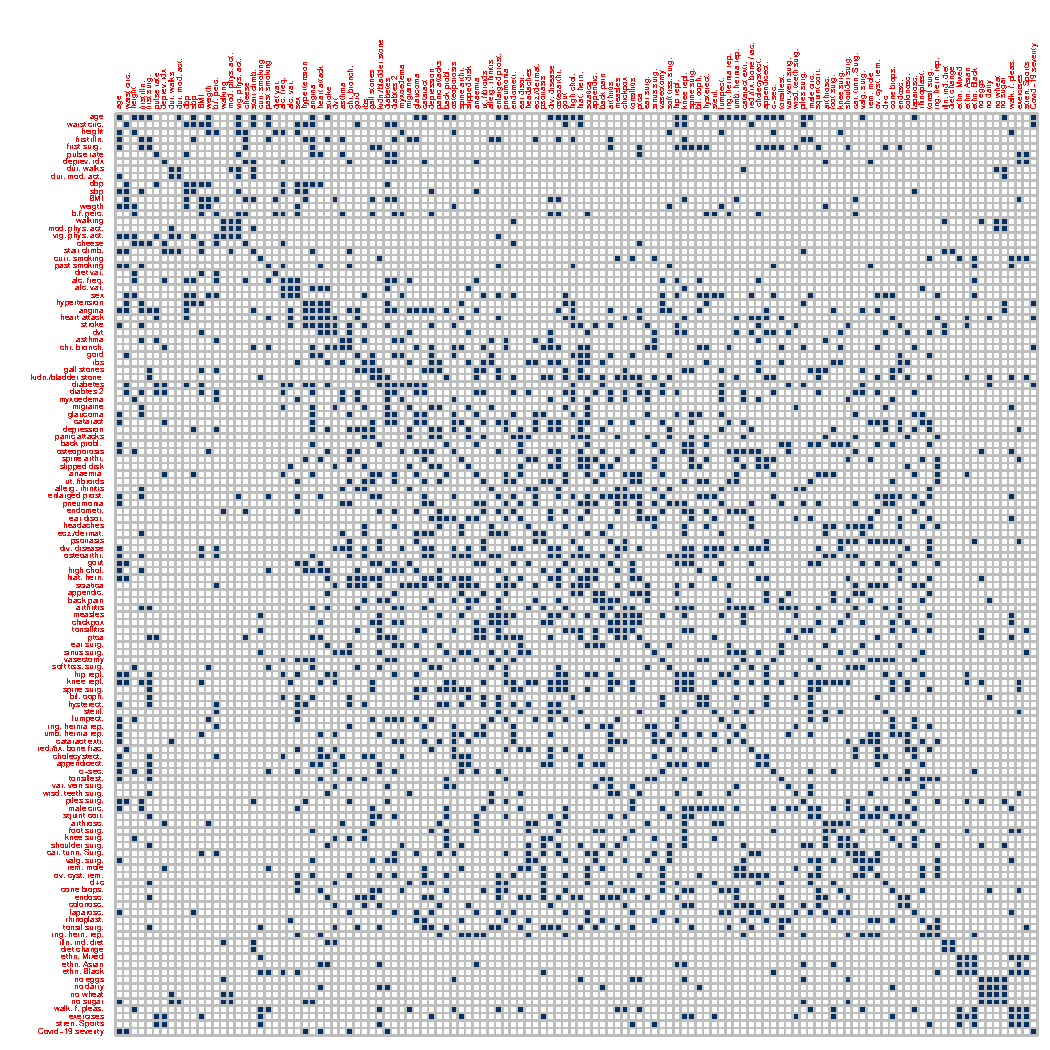
\includegraphics[width=1.0\textwidth]{Figures/corrplot_admat_C.pdf}
    \caption{Plot of the estimated adjacency matrix of data set C.}
    \label{fig:corrplot_admat_C}
\end{figure}

\begin{figure}
    \centering
    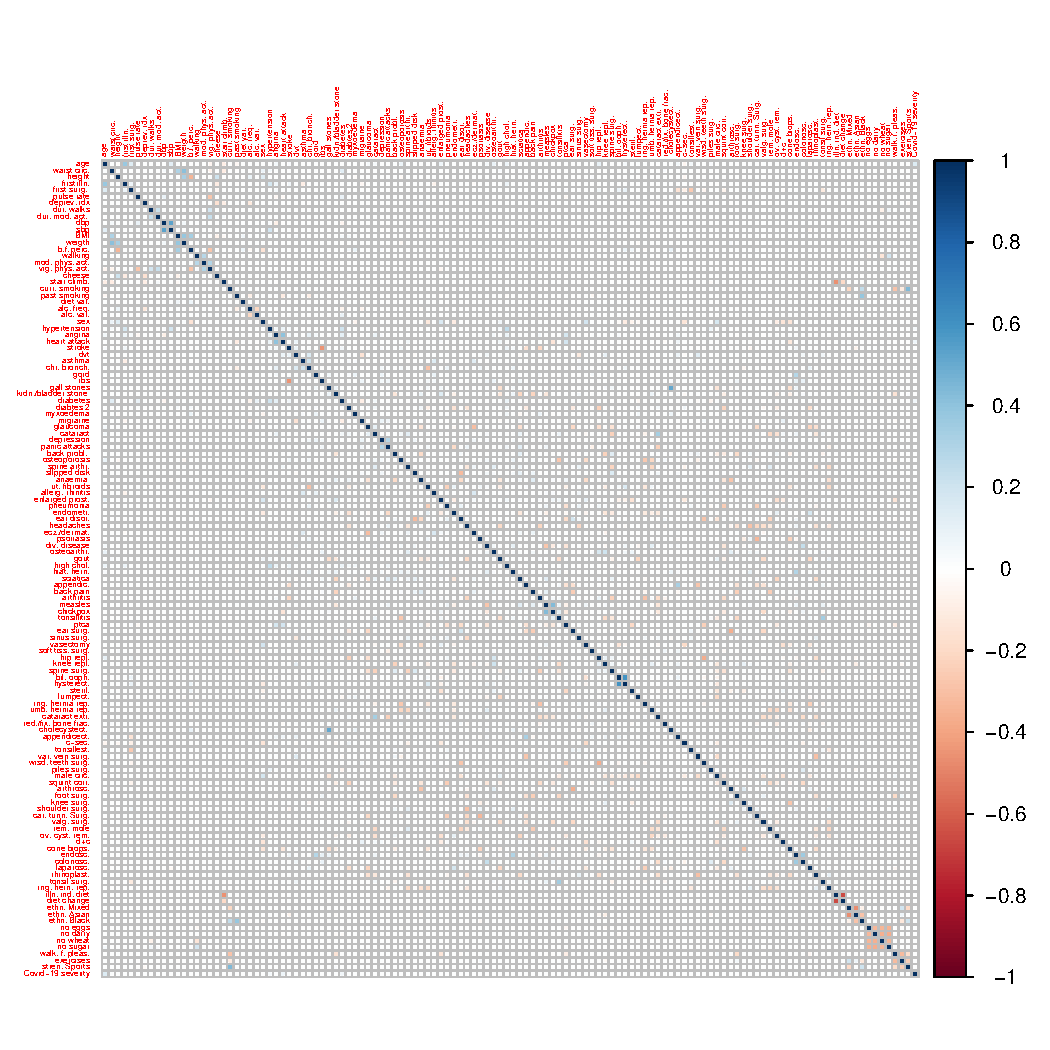
\includegraphics[width=1.0\textwidth]{Figures/corrplot_omega_C.pdf}
    \caption{Plot of the estimated precision matrix of data set C.}
    \label{fig:corrplot_omega_C}
\end{figure}
